\documentclass[12pt,a4paper,dvipdfmx]{jbook} % pLaTeX
%%% LaTeXパッケージのインクルード %%%
\usepackage[utf8]{inputenc}
\usepackage{amssymb}
\usepackage{amsmath}
\usepackage{ascmac}
\usepackage{bm}
\usepackage[x11names,table]{xcolor}
\usepackage{graphicx}
\usepackage{spverbatim} % 折り返し可能なverbを使える
\usepackage{fancyvrb} % verbatim環境の中でitalicを使用するため
\usepackage{wrapfig}
\usepackage{lscape}
\usepackage{setspace}
\usepackage{listings}
\usepackage{here} % 図表をその場に強制的に表示させるため.
\usepackage{hyperref}
\usepackage{pxjahyper}
\usepackage{enumitem}
\usepackage{titlesec}
\usepackage[htt]{hyphenat}
\usepackage[normalem]{ulem}
\usepackage{udline}
\usepackage{fancyhdr}
\usepackage{authblk} % タイトル表示のカスタマイズ
\usepackage{makeidx} % 索引作成
\usepackage{multirow} % 表の行を結合するのに必要
\usepackage{tabularx,booktabs} % 可変サイズの表作成に必要
\usepackage{pdflscape} % Landscape の表の作成のため
\makeindex % 索引作成命令発行

\newcommand{\underbold}[1]{\underline{\bf #1}}
\newcommand{\redtext}[1]{\textcolor{red}{#1}}

%%% ページサイズの設定 %%%
\topmargin=-5mm
\oddsidemargin=-5mm
\evensidemargin=-5mm
\textheight=235mm
\textwidth=165mm

%%% ページのヘッダー・フッターの設定 %%%
% (fancyhdrパッケージが必要)
\pagestyle{fancy}
\lhead{\rightmark}
\chead{}
\rhead{\leftmark}

%%% fancyvrb 環境でitalic体を使用するコマンドを定義 %%%
\newcommand\vrbbf[1]{\textbf{#1}}
\newcommand\vrbit[1]{\textit{#1}}
% <使用方法>
% \begin{Verbatim}[commandchars=\\\{\}]
% \vrbbf{echo foo}
% \vrbit{echo foo} 
% \end{Verbatim}
% ここで、[]のcommandcharsはコマンドに使用する文字列を指定している。
% ここの例だと、\,{,}である。これらの3つの文字の前に\をつけて並べている。
% 詳細は http://tex.stackexchange.com/questions/114942/how-do-i-get-selective-bold-in-verbatim を参照。

%%% カウンター付きのdescription %%%
\newcommand\litem[1]{\item{\bfseries #1\\}}
% <補足>
% 番号はenumerateで生成するので、enumerate環境を使う。
% 番号のスタイルはenumitemパッケージのlabelオプションで変更可能。

%%% subsubsubsection等を定義 %%%
\setcounter{secnumdepth}{5}%
\makeatletter
\newcommand{\subsubsubsection}{\@startsection{paragraph}{4}{\z@}%
{1.5\baselineskip \@plus.5\dp0 \@minus.2\dp0}%
{.5\baselineskip \@plus2.3\dp0}%
{\reset@font\normalsize\bfseries}
}
\newcommand{\subsubsubsubsection}{\@startsection{subparagraph}{5}{\z@}%
{1.5\baselineskip \@plus.5\dp0 \@minus.2\dp0}%
{.5\baselineskip \@plus2.3\dp0}%
{\reset@font\normalsize\itshape}
}
\makeatother
\setcounter{tocdepth}{5}%

%%% footnote の設定 %%%
\renewcommand{\thefootnote}{注\arabic{footnote})}

%%% udline の設定 %%%
%\newcommand{\uwave}[1]{{\setnami\uc{#1}}}
\newcommand{\usaw}[1]{{\setnoko\uc{#1}}}

%%% hyperref 環境の設定 %%%
\hypersetup{%
setpagesize=false,%
bookmarksnumbered=true,%
bookmarksopen=true,%
colorlinks=true,%
linkcolor=blue,%
citecolor=red,%
}%

%%% lstlisting 環境の設定 %%%
\lstdefinelanguage[03fdps]{Fortran}[03]{Fortran}{%
numbers = left,%
numbersep = 8pt,%
numberstyle = \ttfamily\footnotesize,
breaklines = true,%
breakindent = 40pt,%
frame = lines,%
escapeinside={||},%
mathescape=false,%
moredelim=*[directive]\#,%
directives={define,elif,else,endif,error,if,ifdef,ifndef,line,include,pragma,undef,warning},%
basicstyle = \ttfamily\footnotesize,% 基本スタイル
commentstyle=\color[rgb]{0,0,0.8}\ttfamily\footnotesize,% コメント
directivestyle=\color[rgb]{0.83,0.26,0.82}\ttfamily\footnotesize,% マクロ定義
stringstyle=\color[rgb]{0.76,0.22,0.16}\ttfamily\footnotesize,% 文字列
keywordstyle=\color[rgb]{0.05,0.49,0.07}\ttfamily\footnotesize,% void,struct等のキーワード
emph = {c_int,c_short,c_long,c_long_long,c_signed_char,c_size_t,c_int8_t,c_int16_t,c_int32_t,c_int64_t,c_int_least8_t,c_int_least16_t,c_int_least32_t,c_int_least64_t,c_int_fast8_t,c_int_fast16_t,c_int_fast32_t,c_int_fast64_t,c_intmax_t,c_intptr_t,c_float,c_double,c_long_double,c_float_double,c_double_complex,c_long_double_complex,c_bool,c_char,c_null_char,c_alert,c_backspace,c_form_feed,c_new_line,c_carriage_return,c_horizontal_tab,c_vertical_tab,c_null_ptr,c_null_funptr}, %
emphstyle=\color[rgb]{0.83,0.18,0.18}\ttfamily\footnotesize,% その他のキーワード
}[keywords,comments,strings,directives]%
\lstset{%
language = [03fdps]Fortran,%
}

%%% API仕様記述のためのマクロ(牧野さん作成) %%%
\newcommand{\apitop}[1]{
\subsection{#1}
\begin{screen}
}  

\newcommand{\apibottom}[3]{
\end{screen}

\subsubsection*{仮引数仕様}
\begin{table}[H] 
\begin{tabularx}{\linewidth}{cXcX}
\toprule
\rowcolor{Snow2}
仮引数名 & データ型 & 入出力属性 & 定義 \\
\midrule
#1
\bottomrule
\end{tabularx}
\end{table}


% 返り値
\subsubsection*{返り値}
#2


% 機能
\subsubsection*{機能}
#3

}  
\newcommand{\apibottomnoarg}[2]{
\end{screen}

\subsubsection*{仮引数仕様}

なし。
% 返り値
\subsubsection*{返り値}
#1
% 機能
\subsubsection*{機能}
#2

}  

% タイトル、著者、作成日の情報
\title{FDPS Fortran/C言語 インタフェース 仕様書}
\author{行方大輔}
\author{岩澤全規}
\author{似鳥啓吾}
\author{谷川衝}
\author{村主崇行}
\author{Long Wang}
\author{細野七月}
\author{野村昴太郎}
\author{牧野淳一郎}
\affil{理化学研究所 計算科学研究センター 粒子系シミュレータ研究チーム}
\date{}

% 文書の開始
\begin{document}

% タイトルと目次の出力
\maketitle
\tableofcontents

\newpage

%%%%%%%%%%%%%%%%%%%%%%%%%%%%%%%%%%%%%%%%%%%%%%%%%%%%%
\chapter{この文書について}
\label{chap:about}
%%%
\section{文書の構成}
\label{sec:structure}
This document is the specification of FDPS (Framework for Developing Particle Simulator) Fortran/C interface, which supports the development of massively parallel particle simulation codes in Fortran language. This document is written by Daisuke Namekata, Masaki Iwasawa, Ataru Tanikawa, Keigo Nitadori, Takayuki Muranushi, Long Wang, Natsuki Hosono, and Junichiro Makino at RIKEN Center for Computational Science.

This document is structured as follows.

In sections \ref{chap:overview}, \ref{chap:file_str_and_ftn_if_overview}, and \ref{chap:compile_and_macro}, we present prerequisites for programing with FDPS Fortran/C interface. In section \ref{chap:overview}, we show the concept of FDPS. In section \ref{chap:file_str_and_ftn_if_overview}, we present the file configuration of FDPS and FDPS Fortran/C interface. In section \ref{chap:compile_and_macro}, we describe how to compile simulation codes with FDPS.

In sections \ref{chap:data_types}, \ref{chap:user_defined}, and \ref{chap:API_spec_list}, we present information to develop simulation codes with FDPS. In section \ref{chap:data_types}, we described data types defined in FDPS Fortran/C interface. In section \ref{chap:user_defined}, we introduce user-defined types and user-defined functions required for developing codes with FDPS Fortran/C interface. In section \ref{chap:API_spec_list}, we describe APIs used to initialize and finalize FDPS. In section 9, we present modules in FDPS and their APIs.

In sections \ref{chap:error_messages} and \ref{chap:limitation}, we present troubleshooting information. In section \ref{chap:error_messages}, we describe error messages output by both FDPS and FDPS Fortran/C interface. In section \ref{chap:limitation}, we describe the limitation of FDPS and FDPS Fortran/C interface.

Finally, we describe the change log of this document in section \ref{chap:change_log}.
\newpage
%%%
\section{ライセンス}
\label{sec:license}
MITライセンスに準ずる。標準機能のみ使用する場合は、Iwasawa et al. (PASJ, 68, 54)、Namekata et al. (in prep)の引用をお願いします。

拡張機能のParticle MeshクラスはGreeMコード(開発者:石山智明、似鳥啓吾) (Ishiyama, Fukushige \& Makino 2009, Publications of the Astronomical Society of Japan, 61, 1319; Ishiyama, Nitadori \& Makino, 2012 SC'12 Proceedings of the International Conference on High Performance Computing, Networking Stroage and Analysis, No. 5)のモジュールを使用している。GreeMコードはYoshikawa \& Fukushige (2005, Publications of the Astronomical Society of Japan, 57, 849)で書かれたコードをベースとしている。Particle Meshクラスを使用している場合は、上記3つの文献の引用をお願いします。

拡張機能のうちx86版Phantom-GRAPEを使用する場合はTanikawa et al.(2012, New Astronomy, 17, 82)とTanikawa et al.(2012, New Astronomy, 19, 74)の引用をお願いします。

\vspace{5mm}

Copyright (c) $<$2015-$>$ $<$FDPS development team$>$

\vspace{3mm}

Permission is hereby granted, free of charge, to any person obtaining
a copy of this software and associated documentation files (the
``Software''), to deal in the Software without restriction, including
without limitation the rights to use, copy, modify, merge, publish,
distribute, sublicense, and/or sell copies of the Software, and to
permit persons to whom the Software is furnished to do so, subject to
the following conditions:

\vspace{3mm}

The above copyright notice and this permission notice shall be
included in all copies or substantial portions of the Software.

\vspace{3mm}

THE SOFTWARE IS PROVIDED ``AS IS'', WITHOUT WARRANTY OF ANY KIND,
EXPRESS OR IMPLIED, INCLUDING BUT NOT LIMITED TO THE WARRANTIES OF
MERCHANTABILITY, FITNESS FOR A PARTICULAR PURPOSE AND
NONINFRINGEMENT. IN NO EVENT SHALL THE AUTHORS OR COPYRIGHT HOLDERS BE
LIABLE FOR ANY CLAIM, DAMAGES OR OTHER LIABILITY, WHETHER IN AN ACTION
OF CONTRACT, TORT OR OTHERWISE, ARISING FROM, OUT OF OR IN CONNECTION
WITH THE SOFTWARE OR THE USE OR OTHER DEALINGS IN THE SOFTWARE.

\newpage
%%%
\section{ユーザーサポート}
\label{sec:user_support}
Please contact us if you have problems in the development of your code using FDPS Fortran/C interface. The e-mail address is \href{mailto:fdps-support@mail.jmlab.jp}{fdps-support$<$at$>$mail.jmlab.jp} (Please replace \texttt{<at>} by @).

In the following cases, please follow our instructions described below.

%%%%%%%%%%%%%%%%%%%%%%%%%%%%%%%%
\subsection{When you cannot compile your codes}
Please give us the following information:
\begin{itemize}
\item Information about the compiler and libraries used (e.g. their names and versions, and the compile options used)
\item Error messages from the compiler
\item Source codes if possible
\end{itemize}

%%%%%%%%%%%%%%%%%%%%%%%%%%%%%%%%
\subsection{When your code doesn't run as expected}
Please give us the following information:
\begin{itemize}
\item Information about the execution environment (e.g. the name and the version of OS)
\item Rumtime error messages
\item Source codes if possible
\end{itemize}

%%%%%%%%%%%%%%%%%%%%%%%%%%%%%%%%
\subsection{Others}
Please do not hesitate to contact us if you have a problem concerning optimization or other questions. We sincerely hope that you'll find FDPS useful for your research.

\newpage


%%%%%%%%%%%%%%%%%%%%%%%%%%%%%%%%%%%%%%%%%%%%%%%%%%%%%
\chapter{FDPS概要}
\label{chap:overview}
%%この節ではFDPSの概要を記述する。FDPSの開発目的、FDPSの基本的な考えか
%%た、FDPSを使用して作成したコードの動作について概説する。
In this section, we present the design concept of FDPS: the purpose of
its development, the basic concept, and the behavior of codes
developed using FDPS.

%%%%%%%%%%%%%%%%%%%%%%%%%%%%%%%%%%%%%%%%%%%%%%%%%%%%%%%%%%%%%%%%%%%%%%
%\subsection{開発目的}
\subsection{Purpose of the development of FDPS}

%%粒子シミュレーションは、重力$N$体シミュレーション、SPHシミュレーショ
%%ン、渦糸法、MPS法、分子動力学シミュレーションなど理学工学の様々な分野
%%で使用されている。より大きい空間スケール、より高い空間分解能(または質
%%量分解能)、より長い時間スケールの物理現象を追跡するために、高性能な粒
%%子シミュレーションコードへの要請はますます強くなっている。
In the fields of science and engineering, particle method is used for
a wide variety of simulations, such as gravitational $N$-body
simulation, Smoothed Particle Hydrodynamics (SPH) simulation, vortex
method, Moving Particle Semi-implicit (MPS) method, molecular
dynamics simulation, and so on. We need high-performance particle
simulation codes in order to follow physical phenomena with high
spatial resolution, and for long timescales.

%%高性能な粒子シミュレーションコードを組むためには、シミュレーションコー
%%ドの大規模並列化を避けることはできない。粒子シミュレーションコードの
%%大規模並列化をする際には、ロードバランスのため動的領域分割、領域分割
%%に合わせた粒子交換、ノード間通信の削減と最適化、キャッシュ利用効率の
%%向上、SIMDユニット利用効率の向上、アクセラレータへの対応など、数多く
%%の困難な処理を行う必要がある。現在、研究グループは個別にこれらの処理
%%へ対応している。
We cannot avoid parallelization in order to develop high-performance
particle simulation codes. For the parallelization, we need to
implement the following procedures: dynamic domain decomposition for
load balancing, exchange of particles between computing nodes,
optimization of communication among nodes, effective use of cache
memories and SIMD operation units, and support for accelerators. So
far, individual research groups were trying to implement these
procedures.

%%しかし、上記の処理は粒子シミュレーション共通のものである。FDPSの開発
%%目的は、これらの処理を高速に行うライブラリを提供し、大規模並列化への
%%対応に追われていた研究者の負担を軽くすることである。FDPSを使うことで、
%%研究者がよりクリエイティブな仕事に専念できるようになれば、幸いである。
However, the above procedures are necessary for any particle
simulation codes. The purpose of the development of FDPS is to provide
numerical libraries for implementing these procedures, and reduce
researchers' and programmers' burdens. We will be happy if researchers
and programmers can use their time more creatively by making use of
FDPS.

%%%%%%%%%%%%%%%%%%%%%%%%%%%%%%%%%%%%%%%%%%%%%%%%%%%%%%%%%%%%%%%%%%%%%%
%\subsection{基本的な考えかた}
\subsection{Basic concept}

%ここではFDPSの基本的な考えかたについて記述する。
In this section, we describe the basic concept of FDPS.

%%%%%%%%%%%%%%%%%%%%%%%%%%%%%%%%%%%%%%%%%%%%%%%%%%%%
%\subsubsection{大規模並列粒子シミュレーションの手順}
\subsubsection{Procedures of massively parallel particle simulations}
\label{sec:overview_concept_abstraktion}

%%まずFDPSにおいて、大規模並列粒子シミュレーションがどのような手順で行
%%われることを想定しているかを記述する。粒子シミュレーションは、以下の
%%ような微分方程式を時間発展させるものである。
First, we describe our model of massively parallel particle
simulations on FDPS. In particle simulations, the set of ordinary
differential equations,
\begin{align}
    \frac{d\bm{u}_i}{dt} = \sum_j f(\bm{u}_i,\bm{u}_j) + \sum_s
    g(\bm{u}_i,\bm{v}_s), \label{eq:GoverningEquation}
\end{align}
%%ここで$\bm{u}_i$は粒子$i$の物理量ベクトルであり、この物理量には質量、
%%位置、速度など粒子が持つあらゆる物理量が含まれる。関数$f$は粒子$j$か
%%ら粒子$i$への作用を規定する。以後、作用を受ける粒子を$i$粒子、作用を
%%与える粒子を$j$粒子と呼ぶことにする。$\bm{v}_s$は$i$粒子から十分遠方
%%にある粒子を1つの粒子としてまとめた粒子(以後、この粒子を超粒子と呼
%%ぶ)の物理量ベクトルである。関数$g$は超粒子から$i$粒子への作用を規定す
%%る。式(\ref{eq:GoverningEquation})の第2項は、重力やクーロン力など無
%%限遠まで到達する長距離力の場合はゼロではない。しかし流体の圧力のよう
%%な短距離力はゼロである。
is numerically integrated, where $\bm{u}_i$ is the quantity vector of
$i$-particle. This vector includes quantities of particle $i$, such as
mass, position, and velocity. The function $f$ specifies a force
exerted by particle $j$ on particle $i$. Hereafter, a particle
receiving a force is called $i$-particle, and a particle exerting a
force is called particle $j$. The vector $\bm{v}_s$ is the quantity
vector of a superparticle which is the representative particle of a
group of particles distant from $i$-particle. The function $g$
specifies a force exerted by a superparticle on a particle. The second
term in the left hand side of eq.~(\ref{eq:GoverningEquation}) is
non-zero in the case of long-range forces (e.g. gravity and Coulomb
force), while it is zero in the case of short-range forces
(e.g. pressure of fluid).

%%大規模並列化された粒子シミュレーションコードは以下の手順で式
%%(\ref{eq:GoverningEquation})を時間発展させる。ここではデータの入出力
%%や初期化は省略している。
Massively parallel simulation codes integrate the above
eq.~(\ref{eq:GoverningEquation}) in the following steps (initialization
and data I/O are omitted).
\begin{enumerate}
%%\item 以下の2段階の手順でどのプロセスがどの粒子の式
%%(\ref{eq:GoverningEquation})を時間発展させるか決める。
%%\label{item:LoadBalance}
\item In the following two steps, we determine which MPI process
  handles which particles.
  \label{item:LoadBalance}
  \begin{enumerate}
%%  \item プロセスの間でロードバランスを取れるように、シミュレーション
%%  で 扱っている空間の領域を分割し、各プロセスの担当領域を決める(領域
%%  分 割)。
  \item Decompose the whole domain into subdomains, and determine
    which MPI process handles which subdomains, in order to balance
    the calculation cost (domain decomposition).
%%  \item 各プロセスが、自分の担当する領域に存在する全粒子の物理量ベク
%%  ト ル$\bm{u}_i$を持つように、他のプロセスと物理量ベクトル
%%  $\bm{u}_i$を交換する(粒子交換)。
  \item MPI processes exchange their particles in order for each MPI
    process to have particles in its subdomain.
  \end{enumerate}

%%\item 各プロセスは、自分の担当する全粒子の式
%%(\ref{eq:GoverningEquation})の右辺を計算するのに必要な$j$粒子の物理
%%量ベクトル$\bm{u}_j$と超粒子の物理量ベクトル$\bm{v}_s$を他のプロセス
%%と通信することで集めて、$j$粒子のリストと超粒子のリスト(まとめて相互
%%作用リストと呼ぶ)を作る(相互作用リストの作成)。
\item Each MPI process gathers quantity vectors of $j$-particles
  ($\bm{u}_j$) and superparticles ($\bm{v}_s$) required to calculate
  forces exerted on $i$-th $i$-particle (making interaction lists).
  \label{item:MakeInteractionList}

%%\item 各プロセスは自分の担当する全粒子に対して、式
%%(\ref{eq:GoverningEquation})の右辺を計算し、$d\bm{u}_i/dt$を求める(相
%%互作用の計算)。
  \item Each MPI process calculates the right hand of
    eq.~(\ref{eq:GoverningEquation}) for all of its $i$-particle and
    obtains $d\bm{u}_i/dt$.
  \label{item:CalcInteraction}

%%\item 各プロセスは、自分の担当する全粒子の物理量ベクトル$\bm{u}_i$と
%%その時間導関数$d\bm{u}_i/dt$を使って、全粒子の時間積分を実行し、次の
%%時刻の物理量ベクトル$\bm{u}_i$を求める(時間積分)。
\item Each MPI process performes the time integration of its $i$-particles
  by using quantity vectors of $\bm{u}_i$ and their
  derivatives $d\bm{u}_i/dt$.
  \label{item:IntegrateTime}

%\item 手順\ref{item:LoadBalance}に戻る。        
\item Return to step~\ref{item:LoadBalance}.
\end{enumerate}

%%    ただし、あらゆる相互作用のタイプに対応するには以下5種類の$j$粒子
%%    と超粒子の集め方が必要。\label{item:MakeInteractionList}    
%%    \begin{itemize}
%%        \item 長距離力モード:$i$粒子に対して、近い粒子は$j$粒子として、
%%        遠方の複数の粒子はまとめて超粒子として集めるモード(使用例:開
%%        放条件下の重力やクーロン力)
%%        \item 長距離力モードカットオフ付き:長距離力モードとほぼ同じだ
%%        が、ある距離より遠い粒子は集めないモード(使用例:周期境界条件
%%        下の重力やクーロン力)
%%        \item 短距離力収集モード:$i$粒子自身の持つサーチ半径の内側に
%%        ある粒子のみ$j$粒子として集めるモード(使用例:SPH法における密
%%        度の計算)
%%        \item 短距離力散乱モード:$i$粒子をサーチ半径の内側に含む粒子
%%        を$j$粒子として集めるモード(使用例:Lennard-Jones力)
%%        \item 短距離力対称モード:短距離力収集モードで集める粒子と短距
%%        離力散乱モードで集める粒子の和集合を$j$粒子として集めるモード
%%        (使用例:SPH法における圧力勾配の計算)    
%%    \end{itemize}

%%%%%%%%%%%%%%%%%%%%%%%%%%%%%%%%%%%%%%%%%%%%%%%%%%%%
%%\subsubsection{ユーザーとFDPSの役割分担}
\subsubsection{Division of tasks between users and FDPS}

%%FDPSは、プロセス間の通信が発生する処理はFDPSが担当し、プロセス間の通
%%信の発生しない処理はユーザーが担当するという役割分担を基本としている。
%%従って、前節に挙げた、領域分割・粒子交換(項目\ref{item:LoadBalance})・
%%相互作用リストの作成(項目\ref{item:MakeInteractionList})をFDPSが、相
%%互作用の計算(項目\ref{item:CalcInteraction})・時間積分(項目
%%\ref{item:IntegrateTime})をユーザーが担当することになる。ユーザーは
%%FDPSのAPIを呼び出すだけで、大規模並列化に関わる煩雑な処理を避けつつ、
%%高性能な任意の相互作用の粒子シミュレーションコードを手に入れることが
%%できる。
FDPS handles tasks related to interaction calculation and its
efficient parallelization and the user-written code performs the rest.
The actual function for interaction calculation is supplied by
users. Thus, FDPS deals with domain decomposition and exchange of
particles (step~\ref{item:LoadBalance}), and making interaction
lists. On the other hand, the user code is responsible for actual
calculation of forces (step~\ref{item:CalcInteraction}), and time
integration (step~\ref{item:IntegrateTime}). Users can avoid the
development of complicated codes necessary to realize massively
parallel program, by utilizing FDPS APIs.

%%%%%%%%%%%%%%%%%%%%%%%%%%%%%%%%%%%%%%%%%%%%%%%%%%%%
%\subsubsection{ユーザーのやること}
\subsubsection{Users' tasks}

%%ユーザーがFDPSを使って粒子シミュレーションコードを作成するときにやる
%%ことは以下の項目である。
Users's tasks are as follows.
\begin{itemize}

%%\item 粒子の定義(節\ref{sec:userdefined})。粒子の持つ物理量(式
%%(\ref{eq:GoverningEquation})で言えば$\bm{u}_i$)の指定。例えば質量、位
%%置、速度、加速度、元素組成、粒子サイズ、など。
\item Define a particle (section~\ref{sec:userdefined}). Users
  need to specify quantities of particles, \textit{i.e.} the quantity vector
  $\bm{u}_i$ in eq.~(\ref{eq:GoverningEquation}), which contains quantities
  such as position, velocity, acceleration, chemical composition, and particle size.

%%\item 相互作用の定義(節\ref{sec:userdefined})。粒子間の相互作用(式
%%(\ref{eq:GoverningEquation})で言えばで関数$f$, $g$)を指定。例えば、重
%%力、クーロン力、圧力、など。
\item Define interaction (section~\ref{sec:userdefined}). Users
  need to specify the interaction between particles, \textit{i.e.} the function
  $f$ and $g$ in eq.~(\ref{eq:GoverningEquation}), such as gravity,
  Coulomb force, and pressure.

%\item FDPSのAPIの呼出(節\ref{sec:initfin}, \ref{sec:module})
\item Call FDPS APIs (setion~\ref{sec:initfin} and \ref{sec:module}).

\item Time integration of particles, diagnostic, output etc.

\end{itemize}

%%%%%%%%%%%%%%%%%%%%%%%%%%%%%%%%%%%%%%%%%%%%%%%%%%%%
%\subsubsection{補足}
\subsubsection{Complement}

%%式(\ref{eq:GoverningEquation})の右辺は2粒子間相互作用の重ね合わせであ
%%る。従って、FDPSのAPIを呼ぶだけでは、3つ以上の粒子の間の相互作用の計
%%算を行うことはできない。しかし、FDPSはネイバーリストを返すAPIを用意し
%%ている。ネイバーリストを用いれば、ユーザーはプロセス間の通信の処理を
%%することなく、このような相互作用の計算をできる。
The right hand side of eq.~(\ref{eq:GoverningEquation}), the
particle-particle interactions, is strictly of two-body nature. FDPS
APIs can not be used to implement three-particle
interactions. However, for example, FDPS has APIs to return neighbor
lists. Users can calculate three- or more-body interactions, using
these neighbor lists.

%%節\ref{sec:overview_concept_abstraktion}で示した手順は、全粒子が同じ
%%時間刻みを持っている。そのため、FDPSのAPIを呼び出すだけでは、独立時間
%%刻みで時間積分を効率的に行うことができない。しかし、上と同じくネイバー
%%リストを返すAPIがあるため、Particle Particle Particle Tree法を用いて
%%独立時間刻みを実装することは可能であろう。
Calculation steps in section~\ref{sec:overview_concept_abstraktion}
imply that all particles have one same timestep. FDPS APIs do not
support individual timestep scheme. However, users can develop a
particle simulation code with individual timestep scheme, using the
Particle Particle Particle Tree method.

%%%%%%%%%%%%%%%%%%%%%%%%%%%%%%%%%%%%%%%%%%%%%%%%%%%%%%%%%%%%%%%%%%%%%%
%\subsection{コードの動作}
\subsection{The structure of a simulation code with FDPS}
\label{sec:overview_action}

%%ここではFDPSを使用して作成したコードの動作の概略を記述する。このコー
%%ドには、4つのモジュールがあることになる。3つはFDPSのモジュールで、
%%1つはユーザー定義のモジュールである。まとめると以下のようになる。
We overview the structure of a simple simulation code written using FDPS.
In a code with FDPS, three FDPS-supplied classes and several user-defined
classes are used.
\begin{itemize}
%%\item 領域クラス:全プロセスが担当する領域の情報と、領域分割を行う
%%API を持つ
\item DomainInfo class. This class contains the information of all the
  subdomains, and APIs for domain decomposition.

%%\item 粒子群クラス:全粒子の情報と、プロセスの間での粒子交換を行う
%%APIを持つ
\item ParticleSystem class. This class contains the information of all
  particles in each MPI process, and APIs for the exchange of
  particles among MPI processes.

%%\item 相互作用ツリークラス:粒子分布から作られたツリー構造と、相互作
%%用リストを作成するAPIを持つ
\item TreeForForce class. This class contains tree structure made from
  particle distribution, and APIs for making interaction lists.

%%\item ユーザー定義クラス:ある1粒子を定義するクラス、粒子間の相互作
%%用を定義する関数オブジェクトを持つ
\item User-defined classes. These classes include the definitions of
  particles and interactions.
\end{itemize}

%%これら4つのモジュールの間で情報がやり取りされる。これは図
%%\ref{fig:brief_interface}で概観できる。図\ref{fig:brief_interface}に
%%示された情報のやりとりは、節\ref{sec:overview_concept_abstraktion}に
%%記述された手順\ref{item:LoadBalance}から\ref{item:CalcInteraction}と、
%%これらの手順以前に行われる手順(手順0とする)に対応する。以下はこれらの
%%手順の詳細な記述である。
These classes communicate with each other. This is illustrated in
fig.~\ref{fig:brief_interface}. The communication in this figure
corresponds to steps 1 and 2, and to initialization (step~0).
\begin{enumerate}
%%\item[0.] ユーザー定義クラスのうち1粒子を定義するクラスが粒子群クラ
%%スへ、粒子間の相互作用を定義する関数オブジェクトが相互作用ツリークラ
%%スへ渡される。これはクラスの継承ではなく、粒子を定義するクラスは粒子
%%群クラスのテンプレート引数として、粒子間の相互作用を定義する関数オブ
%%ジェクトは相互作用ツリークラスのAPIの引数として渡される
\item[0.] Users give a user-defined particle class to
  ParticleSystem class, and a function object to TreeForForce
  class. These are not class inheritance. The particle class is used as
  a template argument of ParticleSystem class, and the function
  object is used as an argument of APIs in TreeForForce class.

%%\item[\ref{item:LoadBalance}.] 以下の2段階でロードバランスを取る
\item[\ref{item:LoadBalance}.] Do load balancing in the following two
  steps.
  \begin{enumerate}
%%\item 領域クラスが持つ領域分割のAPIが呼ばれる。このとき粒子情報が粒子
%%群クラスから領域クラスへ渡される (赤字と赤矢印)
  \item The user code calls APIs for domain decomposition in
    DomainInfo class. Particle information is transfered from
    ParticleSystem class to DomainInfo class (red text and arrows).
%%  \item 粒子群クラスが持つ粒子交換のAPIが呼ばれる。このとき領域情報が
%%  領域クラスから粒子群クラスへ渡される (青字と青矢印)
  \item The user code calls APIs for exchange of particles in
    ParticleSystem class. Information of subdomains is transfered from
    DomainInfo class to ParticleSystem class (blue text and arrows).
  \end{enumerate}

\item[2.] Do the force calculation in the following steps.

\item[(a)] The user code calls force calculation API.

%%\item[\ref{item:MakeInteractionList}.] 相互作用ツリークラスが持つ相互
%%作用リストを作成するAPIが呼ばれる。このとき領域情報が領域クラスから相
%%互作用ツリークラスへ、粒子情報が粒子群クラスから相互作用ツリークラス
%%へ渡される (緑字と緑矢印)
\item[(b)] FDPS makes interaction lists in TreeForForce
  class. Information of subdomains and particles is transferd from
  DomainInfo and ParticleSystem classes (green text and arrows).

%%\item[\ref{item:CalcInteraction}.] 相互作用ツリーククラスが持つ相互作
%%用を定義した関数オブジェクトを呼び出すAPIが呼ばれる。相互作用計算が実
%%行され、相互作用計算の結果が相互作用ツリークラスから粒子群クラスへ渡
%%される (灰色の字と灰色矢印)
\item[(c)] FDPS calls an user-defined function object. This API is
  included in TreeForForce class.  Interactions are calculated, and
  the results are transfered from TreeForForce class to ParticleSystem
  class (gray text and arrows).
\end{enumerate}

\begin{figure}[h]
  \begin{center}
    %    \includegraphics[width=10cm,bb=0 0 600 500]{fig/brief_interface.jpg}
    \includegraphics[width=10cm,bb=0 0 700 700]{fig/illustration/illustration.001.jpg}
  \end{center}
%%  \caption{モジュールインターフェースと情報の流れの模式図。}
  \caption{Illustration of module interface and data transfer.}
  \label{fig:brief_interface}
\end{figure}

\newpage

%%%%%%%%%%%%%%%%%%%%%%%%%%%%%%%%%%%%%%%%%%%%%%%%%%%%%
\chapter{Fortran/C言語 インターフェースのファイル構成と概要}
\label{chap:file_str_and_ftn_if_overview}
この章では、FDPS Fortran/C言語 インターフェースのファイル構成と概要について記述する。はじめに
ソースファイルの構成とインターフェース概要について記述し、その後、ドキュメントとサンプルコードについて記述する。

%%%%%%%%%%%%%%%%%%%%%%%%%%%%%%%%%%%%%%%%%%%%%%%%%%%%
\section{ファイル構成と概要}
%%%%%%%%%%%%%%%%%%%%%%%%%
\subsection{FDPS 本体}
FDPS 本体のソースファイルはディレクトリ \path{src} の下にある。FDPS 本体は C++ で記述されており、FDPS の標準機能関係のソースファイルはすべて \path{src} の 直下にある。FDPS には拡張機能が用意されており、現時点では、Particle Mesh と x86 版 Phantom-GRAPE が実装されている。それぞれのソースファイルが、\path{src/particle_mesh} と \path{src/phantom_GRAPE_x86} にある。これら拡張機能は静的ライブラリとして使用される。そのため、各ディレクトリにおいて、ユーザ自身の手で、静的ライブラリを作成する必要がある。詳細はFDPS本体の仕様書(\path{doc/doc_specs_cpp_ja.pdf})をご覧頂きたい。
%%%%%%%%%%%%%%%%%%%%%%%%%
\subsection{Fortran インターフェース}
\label{subsec:file_str_ftn_if}
前節で述べた機能の内、Fortran から利用可能なのは、FDPS 標準機能(一部 API は除く)と拡張機能 Particle Mesh である。ユーザは Fortran インターフェースプログラムを通して、これらの機能を使用することとなる。この Fortran インターフェースは、ユーザがディレクトリ\path{scripts}の下に置かれたスクリプト\path{gen_ftn_if.py}を実行することで生成される(スクリプトの仕様は第\ref{chap:script_spec}章で解説する)。このインターフェース生成用スクリプトは、FDPSを利用するにあたってユーザ自身が定義(実装)しなければならない派生データ型(\textbf{ユーザ定義型};第\ref{chap:user_defined}章参照)を解析して、インターフェースプログラムを生成する。\uline{\textbf{したがって、ユーザ最初にしなければならないことはユーザ定義型の実装である}}。FDPSのFortran用のインターフェースがライブラリの形ではなく、このようなインターフェースプログラムの生成という形で提供される理由については別途第\ref{subsec:reasons_for_autogen_ftn_if}節で解説する。Fortranでユーザ定義型を実装するのに必要となるFortranファイルが\path{src/fortran_interface/modules}に、インターフェース生成時に設計図として使用されるファイル群が \path{src/fortran_interface/blueprints} に配置されている。

図\ref{fig:FDPS_ftn_if_file_str}に、Fortran用インターフェースプログラムの生成が正常に行われた場合の Fortran インターフェースのファイル構成とその役割を示している。図の破線で囲まれた4つのファイル(\path{FDPS_module.F90}, \path{FDPS_ftn_if.cpp}, \path{FDPS_Manipulators.cpp}, \path{main.cpp})がスクリプトによって生成されるFortranインターフェースプログラムであり、\path{f_main.F90}がユーザ側が用意するプログラムである。図の点線で囲まれたファイル(\path{FDPS_vector.F90}、\path{FDPS_matrix.F90}、\path{FDPS_super_particle.F90}等)は、前述したように、ユーザがユーザ定義型およびユーザ定義関数(第\ref{chap:overview}章参照)を記述するのに必要な派生データ型の定義を与える。以下、それぞれのインターフェースプログラムの役割について説明を行う。

%%% 図:全体のファイル構成
\begin{figure}[h]
\centering
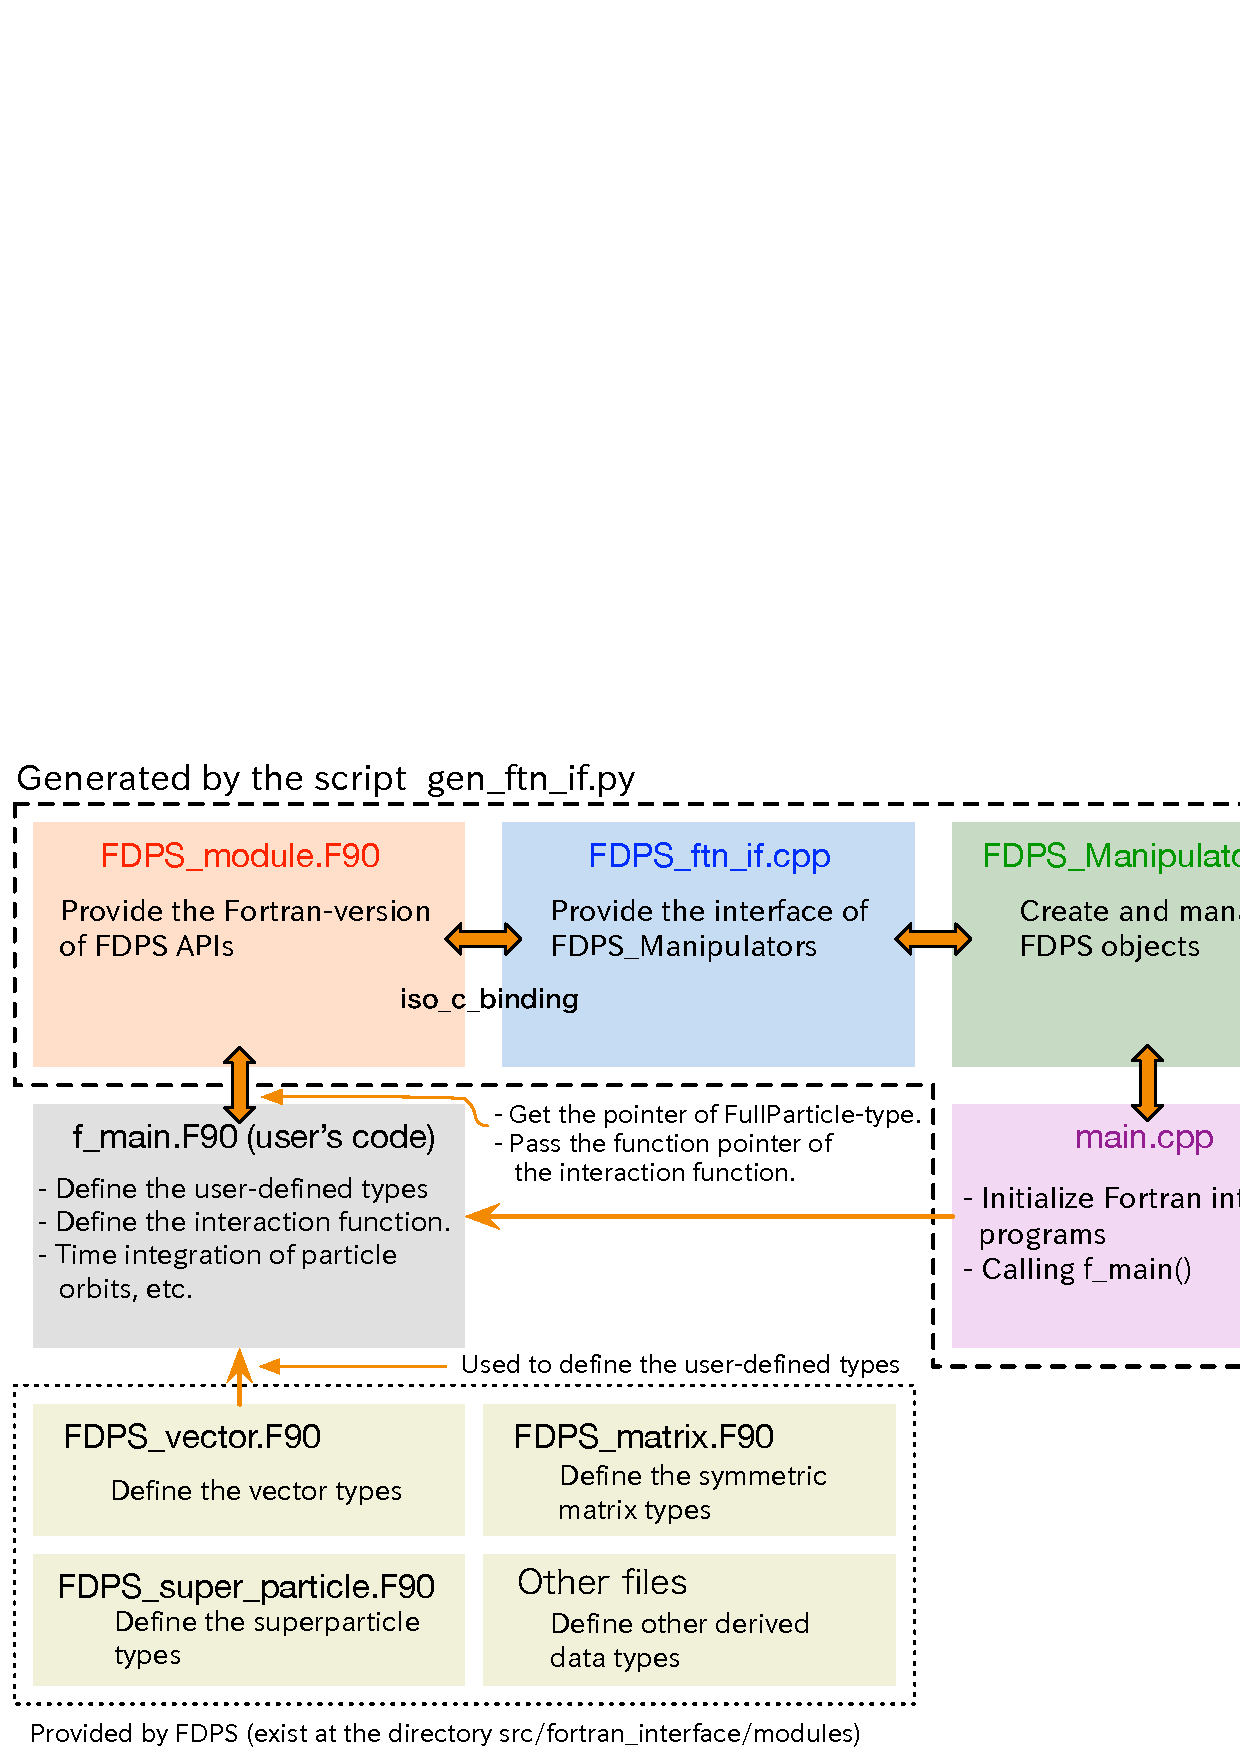
\includegraphics[width=\linewidth]{./fig/FDPS_ftn_if_file_str.pdf}
\caption{Fortran インターフェースとユーザコードの関係。}
\label{fig:FDPS_ftn_if_file_str}
\end{figure}


まず\path{FDPS_Manipulators.cpp}と\path{main.cpp}について説明する。FDPS 本体はC++で記述されているため、第\ref{chap:overview}章「FDPS 概要」で説明した領域クラス、粒子群クラス、相互作用ツリークラスのC++オブジェクトは、すべてC++ファイル内で生成し、管理する必要がある。これを行うのが、\path{FDPS_Manipulators.cpp}である。同様の理由によって、実行プログラムの\path{main}関数はC++ファイルに置く必要がある。そのため、\path{main.cpp}が生成される。この\path{main.cpp}では\path{f_main()}という名称のFortranのサブルーチンを呼び出す。したがって、ユーザはFortran サブルーチン \path{f_main()}を用意し、その中にユーザコードを実装する必要がある。詳細は第\ref{chap:API_spec_list}章「API 仕様一覧」に譲るが、\path{FDPS_Manipulators.cpp}で生成されるC++オブジェクトは、Fortranの整数変数に割り当てられる。したがって、ユーザはこれらのオブジェクトを整数変数を使って管理することとなる。

次に\path{FDPS_ftn_if.cpp}について説明する。FortranはC++の関数を直接呼び出して使用することはできないが、Fortran 2003の機能(Fortranモジュール\path{iso_c_binding}で提供される機能のこと)を使用することで、C言語の関数を呼び出すことが可能になる。そこで、本 FDPS Fortran インターフェースでは、\path{FDPS_Manipulators.cpp}内で定義される各種のC++関数のC言語インターフェースを別途用意し、これらをFortranから呼び出して、FDPSを操作する仕組みとした。これらC言語インターフェースが\path{FDPS_ftn_if.cpp}に実装されている。

最後に、\path{FDPS_module.F90}について説明する。\path{FDPS_module.F90}は、C言語インターフェースを呼び出すための派生データ型\path{FDPS_controller}をユーザに提供する。この\path{FDPS_controller}は、Fortran 2003のクラス(メンバ関数を持つ派生データ型のこと)であり、そのメンバ関数がFDPSのFortran用インターフェースを与える。メンバ関数、すなわち、Fortran インターフェースの一覧は第\ref{chap:API_spec_list}章「API 仕様一覧」で記述する。\path{FDPS_controller}は、\path{FDPS_module.F90}において、以下のように定義されている(リスト\ref{listing:FDPS_module_str}):
\begin{lstlisting}[caption=\texttt{FDPS\_module.F90}の構造,label=listing:FDPS_module_str]
module FDPS_module
   use, intrinsic :: iso_c_binding
   implicit none
   
   !**** FDPS controller
   type, public :: FDPS_controller
   contains
      !
      ! APIs are defined here.
      !
   end type FDPS_controller
   
end module FDPS_module  
\end{lstlisting}
見やすさのため、上記のリストにおいて、メンバ関数の宣言部の記述は省略している。実際には、各メンバ関数の宣言が、文字列\verb|contains|と文字列\verb|end type FDPS_controller|の間の領域に記述される。このような仕様のため、ユーザはユーザコードにおいて、以下の手順でFortranインターフェースを使用する必要がある:
\begin{enumerate}[leftmargin=*,itemsep=-1ex,label=(\arabic*)]
\item モジュール\path{FDPS_module}を\path{use}する
\item クラス\path{FDPS_controller}のオブジェクトを生成する
\item 生成した\path{FDPS_controller}オブジェクトのメンバ関数を呼び出す
\end{enumerate}
最も単純な使用例をリスト\ref{listing:simple_example_ftn_if}に示す:
\begin{lstlisting}[caption=Fortranインターフェースの使用例,label=listing:simple_example_ftn_if]
subroutine f_main()
   use FDPS_module ! Step (1)
   implicit none
   type(FDPS_controller) :: fdps_ctrl ! Step (2)
   
   ! Call Fortran interface
   call fdps_ctrl%PS_initialize() ! Step (3)
   
end subroutine f_main
\end{lstlisting}
リスト中にコメントで示された番号は、上の手順の番号に対応している。

%%%%%%%%%%%%%%%%%%%%%%%%%
\subsection{C言語 インターフェース}
\label{subsec:file_str_c_if}
C言語の場合もFortranの場合と全く同様に、C言語 インターフェースプログラムを通して、FDPSの機能を使用することになる。C言語 インターフェースプログラムの生成は、ユーザがディレクトリ\path{scripts}の下に置かれたスクリプト\path{gen_c_if.py}を実行することで行われる。このスクリプトは、FDPSを利用するにあたってユーザ自身が定義(実装)しなければならない構造体(同様に\textbf{ユーザ定義型}と呼称)を解析して、インターフェースプログラムを生成する。C言語でユーザ定義型を実装するのに必要となるC言語ヘッダーファイルが\path{src/c_interface/headers}に、インターフェース生成時に設計図として使用されるファイル群が \path{src/c_interface/blueprints} に配置されている。

図\ref{fig:FDPS_c_if_file_str}に、C言語用インターフェースプログラムの生成が正常に行われた場合の C言語 インターフェースのファイル構成とその役割を示している。図の破線で囲まれた4つのファイル(\path{FDPS_c_if.h}, \path{FDPS_ftn_if.cpp}, \path{FDPS_Manipulators.cpp}, \path{main.cpp})がスクリプトによって生成されるC言語インターフェースプログラムであり、\path{c_main.c}がユーザ側が用意するプログラムである。図の点線で囲まれたファイル(\path{FDPS_basic.h}、\path{FDPS_enum.h}、\path{FDPS_vector.h}、\path{FDPS_matrix.h}、\path{FDPS_super_particle.h}等)は、前述したように、ユーザがユーザ定義型およびユーザ定義関数(第\ref{chap:overview}章参照)を記述するのに必要な構造体の定義を与えるものである。図からわかるように、ファイル構成は、Fortranインターフェースプログラムと非常に類似した構成となっており(図\ref{fig:FDPS_ftn_if_file_str}参照)、特に同名のファイルの役割はFortranインターフェースで説明したファイルと全く同じである。以下、異なる部分についての注意書きのみを記す。


%%% 図:全体のファイル構成
\begin{figure}[h]
\centering
\includegraphics[width=\linewidth]{./fig/FDPS_c_if_file_str.pdf}
\caption{C言語 インターフェースとユーザコードの関係。}
\label{fig:FDPS_c_if_file_str}
\end{figure}

\begin{itemize}[leftmargin=*]
\item 実行ファイルの\path{main}関数は\path{main.cpp}にある。この\path{main.cpp}では\path{c_main()}という名称の\texttt{void}関数を呼び出す。したがって、ユーザは\texttt{void}関数 \path{c_main()}を用意し、その中にユーザコードを実装する必要がある。
\item FDPSのC言語用APIのプロトタイプ宣言は\path{FDPS_c_if.h}に記述されている。したがって、ユーザはFDPSの機能を利用するため、このファイルをインクルードする必要がある。\path{FDPS_c_if.h}では、FDPSが提供する構造体の定義が記述されたヘッダーファイル群(\path{FDPS_basic.h}等)がインクルードされているため、ユーザはこのファイルのみをインクルードすれば、これら構造体をユーザコードの中で利用することができる。
\end{itemize}


%%%%%%%%%%%%%%%%%%%%%%%%%
\subsection{Fortran/C言語 インターフェースを使ったコード開発の流れ}
本節では、FDPSのFortran/C言語 インターフェースを使ったユーザコード開発の流れについて記述する。大まかな流れは以下のようになる:
\begin{enumerate}[leftmargin=*,label={[\arabic*]}]
\litem{ユーザ定義型の実装} 前節で述べた通り、FDPSのFortran/C言語 インターフェースを生成するためには、はじめにユーザ定義型を実装しなければならない。ユーザ定義型はFortranでFDPSを利用する場合には派生データ型で、C言語でFDPSを利用する場合には構造体として実装する。ユーザ定義型の記述方法の詳細は、第\ref{chap:user_defined}章で説明する。
\litem{インターフェースプログラムの生成} ユーザ定義型の実装が完了したら、インターフェース生成用スクリプト \path{gen_ftn_if.py} または \path{gen_c_if.py} を使って、インターフェースプログラムを生成する。生成が完了した時点で、ユーザはFDPSのFortran/C言語用インターフェースをユーザコードの中で使用することができるようになる。スクリプトの使用法と仕様については第\ref{chap:script_spec}章で説明する。
\litem{ユーザ定義関数の実装} ユーザは相互作用を記述する関数(ユーザ定義関数)を実装しなければならない。ユーザ定義関数は、Fortranではサブルーチン、C言語では\texttt{void}関数として実装する。ユーザ定義関数の記述方法の詳細は、第\ref{chap:user_defined}章で説明する。
\litem{ユーザコードの開発} ユーザ定義型、ユーザ定義関数、FDPS APIを用いて、ユーザが行いたい粒子シミュレーションコードを開発する。この際、次の点に注意して開発を行う必要がある:
\begin{itemize}
\item ユーザコードはFortranのサブルーチン\path{f_main()}、或いは、C言語の\texttt{void}関数 \path{c_main()}の中に実装しなければならない。
\item FDPS Fortran インターフェースのAPIは、クラス\path{FDPS_controller}のメンバ関数として提供される。したがって、FDPS APIはメンバ関数を呼び出して使用する。一方、FDPS C言語 インターフェースのAPIのプロトタイプ宣言は、\path{FDPS_c_if.h}でなされているため、このファイルをインクルードすることでAPIを呼び出すことが可能となる。
\end{itemize}
Fortran インターフェースを用いたコードの例に関しては、\path{sample/fortran}の下で提供されているサンプルコードを参照して頂きたい(第\ref{sec:sample_codes}節も参照のこと)。一方、C言語 インターフェースを用いたサンプルコードは、\path{sample/c}の下に用意されている。
\litem{コンパイル} ユーザコードの実装が完了したら、コンパイルを行い、実行プログラムを得る。前節で述べたように、インターフェースプログラムはC++言語と、Fortran言語或いはC言語のソースファイルが混在した構成となっており、単一の言語のみで構成されたプログラムとは異なる仕方でコンパイルする必要がある。この点に関しての詳細は、第\ref{chap:compile_and_macro}章で解説する。FDPSではコンパイル時のマクロ定義を使い、いくつかの設定を行うことが可能である。これに関しても、第\ref{chap:compile_and_macro}章で解説する。拡張機能 Particle Mesh を使用する場合には、事前に必要なライブラリをインストールし、コンパイル時に適切にライブラリを指定することが必要である。
\litem{実行} コンパイルして得られる実行ファイルは、通常の実行ファイルと違いはない。ユーザが利用している計算機環境の利用規則に則って、実行ファイルを実行する。
\end{enumerate}

%%%%%%%%%%%%%%%%%%%%%%%%%
\subsection{インターフェースプログラム生成の必要性}
\label{subsec:reasons_for_autogen_ftn_if}
前々節で述べたように、FDPSのFortran/C言語用インターフェースはライブラリの形で提供されるものではなく、インターフェースプログラムのソースコードの形で提供される。本節では、この理由について解説を行う。

まず、準備として、C++でのFDPSの使用について概説する。第\ref{chap:overview}章\ref{subsec:things_to_do_by_users}節で述べた通り、FDPSではユーザは粒子や相互作用の定義を自由に行うことができ、これによって、FDPSは様々なタイプの粒子シミュレーションに対して適用可能となっている。この自由度を実現するため、FDPS 本体の関数はC++のテンプレート機能を用いて記述されている。ここで、テンプレート機能とは、Fortranでいうサブルーチンや関数(或いはC言語の関数)に、(変数ではなく)データ型を引数として受け取れるようにする機能のことである。この機能によって、C++では仮のデータ型を使用して関数を記述することが可能となる(この仮のデータ型はコンパイル時に具体的なデータ型になってさえいればよい)。また、FDPS 本体はC++のヘッダファイルの形で提供される。したがって、C++でFDPSを使用する場合、ユーザはFDPSのヘッダファイルをユーザコードの中でインクルードし、FDPS APIのテンプレート引数にユーザが定義した粒子型を指定して使用する。ユーザコードのコンパイル時には、FDPS APIの関数で使用されるすべての変数のデータ型が決定されているため、コンパイラは問題なくユーザプログラムをコンパイルすることが可能となっているのである。

FortranやC言語にはテンプレート機能に相当するものは存在しないため、仮の(或いは、未定の)データ型を用いてサブルーチンや関数を実装する、ということはFortranやC言語では不可能である。これが、Fortran/C言語用インターフェースをライブラリの形で提供できない1つの理由である。我々は、FortranやC言語においてもユーザが粒子や相互作用の定義を自由に行えるようにするため、ユーザが実装した粒子の派生データ型/構造体等を調べ、それに応じて適切なAPIを自動的に生成する方法を採用している。

もう1つの理由は、C++で実装されたFDPSをそのまま使用しているからである。C++で記述されたFDPSとFortran 或いは C言語のプログラムの間でデータをやり取りするためには、FortranやC言語で記述された粒子型と同等な粒子クラスをC++側に用意する必要がある。これにもユーザが実装した派生データ型や構造体を解析して生成するという作業が必要となる。

以上の理由により、FDPS Fortran/C言語 インターフェースは、ソースコードで提供される形となっている。

%%%%%%%%%%%%%%%%%%%%%%%%%%%%%%%%%%%%%%%%%%%%%%%%%%%%
\section{ドキュメント}
ドキュメント関係のファイルはディレクトリ \path{doc} の下にある。サンプルコードを使ってFDPS Fortran インターフェースの基本的な使用法を解説するチュートリアル文書が \path{doc_tutorial_ftn_ja.pdf} である。C言語 インターフェースの基本的な使用方法についてのチュートリアル文書は\path{doc_tutorial_c_ja.pdf}である。仕様書(本文書)が \path{doc_specs_ftn_ja.pdf} である。

%%%%%%%%%%%%%%%%%%%%%%%%%%%%%%%%%%%%%%%%%%%%%%%%%%%%
\section{サンプルコード}
\label{sec:sample_codes}
FortranとC言語のサンプルコードが、それぞれ、ディレクトリ \path{sample/fortran} 及び \path{sample/c} の下にある。サンプルコードは4つ用意されており、それぞれ、無衝突系の重力 $N$ 体シミュレーションコード(\path{sample/fortran/nbody}, \path{sample/c/nbody})、固定長カーネルを使った SPH シミュレーションコード(\path{sample/fortran/sph}, \path{sample/c/sph})、$\mathrm{P^{3}M}$(Particle-Particle-Particle-Mesh) 計算用コード(\path{sample/fortran/p3m}, \path{sample/c/p3m})、円盤銀河の$N$体/SPHシミュレーションコード(\path{sample/fortran/nbody+sph}, \path{sample/c/nbody+sph})となっている。

\newpage

%%%%%%%%%%%%%%%%%%%%%%%%%%%%%%%%%%%%%%%%%%%%%%%%%%%%%
\chapter{FDPSで提供されるデータ型}
\label{chap:data_types}
FDPS Fortran/C interface defines several data types including vector types, symmetric matrix types, superparticle types, time profile type, enum types. In addition, basic data types are also defined in C. These data types are required to be used in user-defined types and user-defined functions (Chap.~\ref{chap:user_defined}) or are used as returned values in some APIs (Chap.~\ref{chap:API_spec_list}).

%%%%%%%%%%%%%%%%%%%%%%%%%%%%%%%%%%%%%%%%%%%%%%%%%%%%%%
\section{Basic data types {\small (C only)}}
\label{sec:basic_types}
FDPS C interface defines six basic data types: \path{fdps_s32}, \path{fdps_u32}, \path{fdps_f32}, \path{fdps_s64}, \path{fdps_u64}, \path{fdps_f64}. They are defined in the file \path{src/c_interface/headers/FDPS_basic.h} as follows (Listing~\ref{listing:basic_types}). These data types are used to defined other data types provided by FDPS.

\begin{lstlisting}[language=C,caption=Basic data types (C only),label=listing:basic_types]
#pragma once

/* 32 bit data types */
typedef int          fdps_s32;
typedef unsigned int fdps_u32;
#ifdef PARTICLE_SIMULATOR_ALL_64BIT_PRECISION
typedef double       fdps_f32;
#else
typedef float        fdps_f32;
#endif

/* 64 bit data types */
typedef long long int          fdps_s64;
typedef unsigned long long int fdps_u64;
typedef double                 fdps_f64;
\end{lstlisting}

\redtext{Note that the macro \texttt{PARTICLE\_SIMULATOR\_ALL\_64BIT\_PRECISION} is just introduced for future and C interface programs work correctly only if this macro is undefined.}

%%%%%%%%%%%%%%%%%%%%%%%%%%%%%%%%%%%%%%%%%%%%%%%%%%%%%%
\section{Vector types}
\label{sec:vector_types}
FDPS Fortran and C interface define two types of vector: \path{fdps_f32vec} and \path{fdps_f64vec}. They are defined in the files \path{src/fortran_interface/modules/FDPS_vector.F90} and \path{src/c_interface/headers/FDPS_vector.h} as follows (Listings~\ref{listing:vector_types} and \ref{listing:vector_types_in_C}). Each vector has 2 or 3 member variables depending on the spatial dimension of the simulation. By default, the spatial dimension of the simulation is assumed to be 3, but it is 2 if the macro \path{PARTICLE_SIMULATOR_TWO_DIMENSION} is defined at the compilation. The data type of the member variables is either 32-bit or 64-bit floating point numbers.

\begin{lstlisting}[caption=Vector types (Fortran),label=listing:vector_types]
module fdps_vector
   use, intrinsic :: iso_c_binding
   implicit none
   
   type, public, bind(c) :: fdps_f32vec
#ifdef PARTICLE_SIMULATOR_TWO_DIMENSION 
      real(kind=c_float) :: x,y
#else
      real(kind=c_float) :: x,y,z
#endif
   end type fdps_f32vec

   type, public, bind(c) :: fdps_f64vec
#ifdef PARTICLE_SIMULATOR_TWO_DIMENSION 
      real(kind=c_double) :: x,y
#else
      real(kind=c_double) :: x,y,z
#endif
   end type fdps_f64vec

end module fdps_vector
\end{lstlisting}

\begin{lstlisting}[language=C,caption=Vector types (C), label=listing:vector_types_in_C]
#pragma once
#include "FDPS_basic.h"

//**** PS::F32vec
typedef struct  {
#ifdef PARTICLE_SIMULATOR_TWO_DIMENSION
   fdps_f32 x,y;
#else
   fdps_f32 x,y,z;
#endif
} fdps_f32vec;

//**** PS::F64vec
typedef struct  {
#ifdef PARTICLE_SIMULATOR_TWO_DIMENSION
   fdps_f64 x,y;
#else
   fdps_f64 x,y,z;
#endif
} fdps_f64vec;
\end{lstlisting}

In Fortran, for the vector types, the definitions of the assignment (\texttt{=}) and the arithmetic operators (\texttt{+},\texttt{-},\texttt{*},\texttt{/}) are extended as shown in Table.~\ref{tbl:op_ext:fdps_vector}. For more details, see \path{FDPS_vector.F90}.

\begin{table}[H]
\begin{tabularx}{\linewidth}{|c|c|c|X|}
\toprule
\rowcolor{Snow2}
Symbol & Left-hand side & Right-hand side & Definition \\
\midrule
% 代入記号(=)
\multirow{3}{*}{\texttt{=}} & vector & scalar$^{\dagger}$ & \multirow{3}{\hsize}{\footnotesize Assign RHS to LHS$^{\sharp}$. When RHS is scalar, it is assigned to all the components of LHS. When RHS is an array, each component of LHS is assigned by array element according to the memory ordering.} \\[2pt]
\cmidrule(r){2-3}
 & vector & array of scalars$^{\ddagger}$ &  \\[2pt]
\cmidrule(r){2-3}
 & vector & vector &  \\[2pt]
\midrule
% + 演算子
\multirow{4}{*}{\texttt{+}} & vector & array of scalars & \multirow{3}{\hsize}{\footnotesize Addition of LHS and RHS. When one of the operands is an array, it is assumed that each element of the array corresponds to the component of the vector according to the memory ordering.} \\[2pt]
\cmidrule(r){2-3}
 & array of scalars & vector & \\[2pt]
\cmidrule(r){2-3}
 & vector & vector & \\[2pt]
\cmidrule(r){2-4}
 & none & vector & Do nothing \\
\midrule
% - 演算子
\multirow{4}{*}{\texttt{-}} & vector & array of scalars & \multirow{3}{\hsize}{\footnotesize Subtraction RHS from LHS. When one of the operands is an array, it is assumed that each element of the array corresponds to the component of the vector according to the memory ordering.} \\[2pt]
\cmidrule(r){2-3}
& array of scalars & vector &  \\[2pt]
\cmidrule(r){2-3}
& vector & vector & \\[2pt]
\cmidrule(r){2-4}
& none & vector & Inversion of the sign of the vector \\
\midrule
% * 演算子
\multirow{5}{*}{\texttt{*}} & vector & scalar & \multirow{2}{*}{Scalar-vector product} \\
\cmidrule(r){2-3}
 & scalar & vector & \\
\cmidrule(r){2-4}
 & vector & array of scalars & \multirow{3}{\hsize}{\footnotesize Inner product. When one of the operands is an array, it is assumed that each element of the array corresponds to the component of the vector according to the memory ordering.} \\
\cmidrule(r){2-3}
 & array of scalars & vector &  \\
\cmidrule(r){2-3}
 & vector & vector &  \\
\midrule
\texttt{/} & vector & scalar & Division LHS by RHS. \\
\bottomrule
\end{tabularx}
\begin{flushleft}
$^{\dagger}$ The data type of scalar must be one of intrinsic data types in Fortran and be numeric. \\
$^{\ddagger}$ The size of array must be 2 if the macro \path{PARTICLE_SIMULATOR_TWO_DIMENSION} is defined at the compilation. Otherwise, it must be 3. \\
$^{\sharp}$ LHS and RHS stand for the left- and the right-hand sides, respectively.
\end{flushleft}
\caption{The definitions of the assignment and the arithmetic operators extended for the vector types}
\label{tbl:op_ext:fdps_vector}
\end{table}


%%%%%%%%%%%%%%%%%%%%%%%%%%%%%%%%%%%%%%%%%%%%%%%%%%%%%%
\section{Symmetric Matrix types}
\label{sec:symmetric_matrix_types}
There are two types of symmetric matrix: \path{fdps_f32mat} and \path{fdps_f64mat}. These are defined in the files \path{src/fortran_interface/modules/FDPS_matrix.F90} and \path{src/c_interface/headers/FDPS_matrix.h} as follows (Listings~\ref{listing:symmetric_matrix_types} and \ref{listing:symmetric_matrix_types_in_C}). Each symmetric matrix type has 3 or 6 member variables depending on the spatial dimension of the simulation. By default, the spatial dimension of the simulation is assumed to be 3, but it is 2 if the macro \path{PARTICLE_SIMULATOR_TWO_DIMENSION} is defined at the compilation. The data type of the member variables is either 32-bit or 64-bit floating point numbers.

\begin{lstlisting}[caption=Symmetric Matrix types (Fortran),label=listing:symmetric_matrix_types]
module fdps_matrix
   use, intrinsic :: iso_c_binding
   implicit none

   !**** PS::F32mat
   type, public, bind(c) :: fdps_f32mat
#ifndef PARTICLE_SIMULATOR_TWO_DIMENSION
      real(kind=c_float) :: xx,yy,zz,xy,xz,yz
#else
      real(kind=c_float) :: xx,yy,xy
#endif
   end type fdps_f32mat

   !**** PS::F64mat
   type, public, bind(c) :: fdps_f64mat
#ifndef PARTICLE_SIMULATOR_TWO_DIMENSION
      real(kind=c_double) :: xx,yy,zz,xy,xz,yz
#else
      real(kind=c_double) :: xx,yy,xy
#endif
   end type fdps_f64mat

end module fdps_matrix  
\end{lstlisting}

\begin{lstlisting}[language=C,caption=Symmetric Matrix types (C), label=listing:symmetric_matrix_types_in_C]
#pragma once
#include "FDPS_basic.h"

//**** PS::F32mat
typedef struct {
#ifndef PARTICLE_SIMULATOR_TWO_DIMENSION
   fdps_f32 xx,yy,zz,xy,xz,yz;
#else
   fdps_f32 xx,yy,xy;
#endif
} fdps_f32mat;

//**** PS::F64mat
typedef struct {
#ifndef PARTICLE_SIMULATOR_TWO_DIMENSION
   fdps_f64 xx,yy,zz,xy,xz,yz;
#else
   fdps_f64 xx,yy,xy;
#endif
} fdps_f64mat;
\end{lstlisting}

In Fortran, for the symmetric matrix types, the definitions of the assignment (\texttt{=}) and the arithmetic operators (\texttt{+},\texttt{-},\texttt{*},\texttt{-}) are extended as shown in Table.~\ref{tbl:op_ext:fdps_matrix}. For more details, see \path{FDPS_matrix.F90}.

\begin{table}[H]
\begin{tabularx}{\linewidth}{|c|c|c|X|}
\toprule
\rowcolor{Snow2}
Symbol & Left-hand side & Right-hand side & Definition \\
\midrule
% = 記号
\multirow{2}{*}{\texttt{=}}& matrix & scalar$^{\dagger}$ & \multirow{2}{\hsize}{\footnotesize Assign RHS to LHS. When RHS is scalar, it is assigned to all the components of LHS.} \\
\cmidrule(r){2-3}
& matrix & matrix & \\
\midrule
% + 演算子
\multirow{2}{*}{\texttt{+}} & matrix & matrix & Addition of LHS and RHS. \\
\cmidrule(r){2-4}
& none & matrix & Do nothing \\
\midrule
% - 演算子
\multirow{2}{*}{\texttt{-}} & matrix & matrix & Subtraction RHS from LHS. \\
\cmidrule(r){2-4}
& none & matrix & {\footnotesize Sign inversion of all the components of the matrix} \\
\midrule
% * 演算子
\multirow{3}{*}{\texttt{*}} & matrix & scalar & \multirow{2}{*}{Scalar-matrix product} \\
\cmidrule(r){2-3}
 & scalar & matrix &  \\
\cmidrule(r){2-4}
 & matrix & matrix & Matrix product \\
\midrule
% / 演算子
\texttt{/} & matrix & scalar & Division LHS by RHS. \\
\bottomrule
\end{tabularx}
\begin{flushleft}
$^{\dagger}$ The data type of scalar must be one of intrinsic data types in Fortran and be numeric.
\end{flushleft}
\caption{The definitions of the assignment and the arithmetic operators extended for the symmetric matrix types}
\label{tbl:op_ext:fdps_matrix}
\end{table}



%%%%%%%%%%%%%%%%%%%%%%%%%%%%%%%%%%%%%%%%%%%%%%%%%%%%%%
\section{Superparticle types}
\label{sec:super_particle_types}
A superparticle is a virtual particle that represents a group of real particles, which are located far from the $i$-particle (a particle which we want to calculate the force acting on). Its properties are computed from the properties of these real particles via some way. Superparticle types are derived data types required to describe the interaction between a particle and a superparticle. They are used in user-defined functions to receive data of superparticles.

The superparticle types include \path{fdps_spj_monopole},\path{fdps_spj_quadrupole},\path{fdps_spj_monopole_geomcen},\path{fdps_spj_dipole_geomcen},\path{fdps_spj_quadrupole_geomcen},\path{fdps_spj_monopole_scatter},\path{fdps_spj_quadrupole_scatter}, \path{fdps_spj_monopole_symmetry}, \path{fdps_spj_quadrupole_symmetry},  \path{fdps_spj_monopole_cutoff}. They are defined in the files \path{src/fortran_interface/modules/FDPS_super_particle.F90} and \path{src/c_interface/headers/FDPS_super_particle.h} as follows (Listings~\ref{listing:superparticle_types} and \ref{listing:superparticle_types_in_C}). Note that the vector types and the symmetric matrix types are used to define the superparticle types.

\begin{lstlisting}[caption=Superparticle types (Fortran),label=listing:superparticle_types]
module fdps_super_particle
   use, intrinsic :: iso_c_binding
   use fdps_vector
   use fdps_matrix
   implicit none

   !**** PS::SPJMonopole
   type, public, bind(c) :: fdps_spj_monopole
      real(kind=c_double) :: mass
      type(fdps_f64vec) :: pos
   end type fdps_spj_monopole

   !**** PS::SPJQuadrupole
   type, public, bind(c) :: fdps_spj_quadrupole
      real(kind=c_double) :: mass
      type(fdps_f64vec)  :: pos
      type(fdps_f64mat)  :: quad
   end type fdps_spj_quadrupole

   !**** PS::SPJMonopoleGeometricCenter
   type, public, bind(c) :: fdps_spj_monopole_geomcen
      integer(kind=c_long_long) :: n_ptcl
      real(kind=c_double) :: charge
      type(fdps_f64vec) :: pos
   end type fdps_spj_monopole_geomcen

   !**** PS::SPJDipoleGeometricCenter
   type, public, bind(c) :: fdps_spj_dipole_geomcen
      integer(kind=c_long_long) :: n_ptcl
      real(kind=c_double) :: charge
      type(fdps_f64vec) :: pos
      type(fdps_f64vec) :: dipole
   end type fdps_spj_dipole_geomcen

   !**** PS::SPJQuadrupoleGeometricCenter
   type, public, bind(c) :: fdps_spj_quadrupole_geomcen
      integer(kind=c_long_long) :: n_ptcl
      real(kind=c_double) :: charge
      type(fdps_f64vec) :: pos
      type(fdps_f64vec) :: dipole
      type(fdps_f64mat) :: quadrupole
   end type fdps_spj_quadrupole_geomcen

   !**** PS::SPJMonopoleScatter
   type, public, bind(c) :: fdps_spj_monopole_scatter
      real(kind=c_double) :: mass
      type(fdps_f64vec) :: pos
   end type fdps_spj_monopole_scatter

   !**** PS::SPJQuadrupoleScatter
   type, public, bind(c) :: fdps_spj_quadrupole_scatter
      real(kind=c_double) :: mass
      type(fdps_f64vec)  :: pos
      type(fdps_f64mat)  :: quad
   end type fdps_spj_quadrupole_scatter

   !**** PS::SPJMonopoleSymmetry
   type, public, bind(c) :: fdps_spj_monopole_symmetry
      real(kind=c_double) :: mass
      type(fdps_f64vec) :: pos
   end type fdps_spj_monopole_symmetry

   !**** PS::SPJQuadrupoleSymmetry
   type, public, bind(c) :: fdps_spj_quadrupole_symmetry
      real(kind=c_double) :: mass
      type(fdps_f64vec) :: pos
      type(fdps_f64mat) :: quad
   end type fdps_spj_quadrupole_symmetry

   !**** PS::SPJMonopoleCutoff
   type, public, bind(c) :: fdps_spj_monopole_cutoff
      real(kind=c_double) :: mass
      type(fdps_f64vec) :: pos
   end type fdps_spj_monopole_cutoff
   
end module fdps_super_particle   
\end{lstlisting}

\begin{lstlisting}[language=C,caption=Superparticle types (C),label=listing:superparticle_types_in_C]
#pragma once
#include "FDPS_basic.h"
#include "FDPS_vector.h"
#include "FDPS_matrix.h"

#ifdef PARTICLE_SIMULATOR_SPMOM_F32
typedef fdps_s32    fdps_sSP;
typedef fdps_f32    fdps_fSP;
typedef fdps_f32vec fdps_fSPvec;
typedef fdps_f32mat fdps_fSPmat;
#else
typedef fdps_s64    fdps_sSP;
typedef fdps_f64    fdps_fSP;
typedef fdps_f64vec fdps_fSPvec;
typedef fdps_f64mat fdps_fSPmat;
#endif

//**** PS::SPJMonopole
typedef struct {
   fdps_fSP mass;
   fdps_fSPvec pos;
} fdps_spj_monopole;

//**** PS::SPJQuadrupole
typedef struct {
   fdps_fSP mass;
   fdps_fSPvec pos;
   fdps_fSPmat quad;
} fdps_spj_quadrupole;

//**** PS::SPJMonopoleGeometricCenter
typedef struct {
   fdps_sSP n_ptcl;
   fdps_fSP charge;
   fdps_fSPvec pos;
} fdps_spj_monopole_geomcen;

//**** PS::SPJDipoleGeometricCenter
typedef struct {
   fdps_sSP n_ptcl;
   fdps_fSP charge;
   fdps_fSPvec pos;
   fdps_fSPvec dipole;
} fdps_spj_dipole_geomcen;

//**** PS::SPJQuadrupoleGeometricCenter
typedef struct {
   fdps_sSP n_ptcl;
   fdps_fSP charge;
   fdps_fSPvec pos;
   fdps_fSPvec dipole;
   fdps_fSPmat quadrupole;
} fdps_spj_quadrupole_geomcen;

//**** PS::SPJMonopoleScatter
typedef struct {
   fdps_fSP mass;
   fdps_fSPvec pos;
} fdps_spj_monopole_scatter;

//**** PS::SPJQuadrupoleScatter
typedef struct {
   fdps_fSP mass;
   fdps_fSPvec pos;
   fdps_fSPmat quad;
} fdps_spj_quadrupole_scatter;

//**** PS::SPJMonopoleSymmetry
typedef struct {
   fdps_fSP mass;
   fdps_fSPvec pos;
} fdps_spj_monopole_symmetry;

//**** PS::SPJQuadrupoleSymmetry
typedef struct {
   fdps_fSP mass;
   fdps_fSPvec pos;
   fdps_fSPmat quad;
} fdps_spj_quadrupole_symmetry;

//**** PS::SPJMonopoleCutoff
typedef struct {
   fdps_fSP mass;
   fdps_fSPvec pos;
} fdps_spj_monopole_cutoff;
\end{lstlisting}

There is an one-to-one correspondence between the superparticle types and the types of tree objects. Accordingly, users must use an appropriate superparticle type corresponding to the type of created tree object. The correspondence relationship between the types of tree objects and the superparticle types is shown in Table~\ref{tbl:tree_and_super_particle}. Note that the types of tree object for short-range force are not shown in this table, because superparticle is only used in the case of long-range force. For the other types of tree object and the way to create tree objects, see Chap.~\ref{chap:API_spec_list} \S~\ref{sec:tree_APIs}.

\begin{landscape}
\begin{table}[h]
\begin{tabularx}{\hsize}{lp{5cm}Xl}
\toprule
\rowcolor{Snow2}
Tree type & Highest-order of multipole moments$^{\dagger}$ & Range of interaction & Superparticle type \\
\midrule
Long-Monopole type & monopole(CoM) & Entire region & \path{fdps_spj_monopole} \\
\midrule
Long-Quadrupole type & quadrupole(CoM) & Entire region & \path{fdps_spj_quadrupole} \\
\midrule
Long-MonopoleGeometricCenter type & monopole(GC) & Entire region & \path{fdps_spj_monopole_geomcen} \\
\midrule
Long-DipoleGeometricCenter type & dipole(GC) & Entire region & \path{fdps_spj_dipole_geomcen} \\
\midrule
Long-QuadrupoleGeometricCenter type & quadrupole(GC) & Entire region & \path{fdps_spj_quadrupole_geomcen} \\
\midrule
Long-MonopoleWithScatterSearch type$^{\ddagger}$ & monopole(CoM) & Entire region & \path{fdps_spj_monopole_scatter} \\
\midrule
Long-QuadrupoleWithScatterSearch type$^{\ddagger}$ & quadrupole(CoM) & Entire region & \path{fdps_spj_quadrupole_scatter} \\
\midrule
Long-MonopoleWithSymmetrySearch type$^{\ddagger}$ & monopole(CoM) & Entire region & \path{fdps_spj_monopole_symmetry} \\
\midrule
Long-QuadrupoleWithSymmetrySearch type$^{\ddagger}$ & quadrupole(CoM) & Entire region & \path{fdps_spj_quadrupole_symmetry} \\
\midrule
Long-MonopoleWithCutoff type & monopole(CoM) & Within cutoff radius & \path{fdps_spj_monopole_cutoff} \\
\bottomrule
\end{tabularx}
\begin{flushleft}
$^{\dagger}$ CoM indicates that multipole moments are calculated assuming that the center-of-mass is the center of the expansion. GC indicates that multipole moments are calculated assuming that the geometric center is the center of the expansion. \\
$^{\ddagger}$ Scatter- or Symmetry-mode neighbor search is possible. In the calculation of interaction, neighbor particles are forcibly treated as normal particles. In other words, superparticles do not have neighbor particles as members.
\end{flushleft}
\caption{The correspondence relationship between the types of tree for long-range force and the superparticle types}
\label{tbl:tree_and_super_particle}
\end{table}
\end{landscape}


%%%%%%%%%%%%%%%%%%%%%%%%%%%%%%%%%%%%%%%%%%%%%%%%%%%%%%
\section{Time profile types}
\label{sec:time_profile_types}
Time profile types are used to obtain the elapsed times of various types of calculations performed in FDPS. At present, there is only one time profile type \path{fdps_time_profile}. It is defined in the files \path{src/fortran_interface/modules/FDPS_time_profile.F90} and \path{src/c_interface/headers/FDPS_time_profile.h} as follows (Listings~\ref{listing:time_profile_types} and \ref{listing:time_profile_types_in_C}). This data type is exclusively used by the APIs for time measurement (for detail, see Chap.~\ref{chap:API_spec_list}).

\begin{lstlisting}[caption=Time profile types (Fortran),label=listing:time_profile_types]
module fdps_time_profile
   use, intrinsic :: iso_c_binding
   implicit none

   !**** PS::TimeProfile
   type, public, bind(c) :: fdps_time_prof
      real(kind=c_double) :: collect_sample_particle
      real(kind=c_double) :: decompose_domain
      real(kind=c_double) :: exchange_particle
      real(kind=c_double) :: set_particle_local_tree
      real(kind=c_double) :: set_particle_global_tree
      real(kind=c_double) :: make_local_tree
      real(kind=c_double) :: make_global_tree
      real(kind=c_double) :: set_root_cell
      real(kind=c_double) :: calc_force
      real(kind=c_double) :: calc_moment_local_tree
      real(kind=c_double) :: calc_moment_global_tree
      real(kind=c_double) :: make_LET_1st
      real(kind=c_double) :: make_LET_2nd
      real(kind=c_double) :: exchange_LET_1st
      real(kind=c_double) :: exchange_LET_2nd
                                                                                                   
      real(kind=c_double) :: morton_sort_local_tree                                                
      real(kind=c_double) :: link_cell_local_tree                                                  
      real(kind=c_double) :: morton_sort_global_tree                                               
      real(kind=c_double) :: link_cell_global_tree                                                 
                                                                                                   
      real(kind=c_double) :: make_local_tree_tot                                                   
      ! = make_local_tree + calc_moment_local_tree                                                 
      real(kind=c_double) :: make_global_tree_tot                                                  
      real(kind=c_double) :: exchange_LET_tot                                                      
      ! = make_LET_1st + make_LET_2nd + exchange_LET_1st + exchange_LET_2nd                        
                                                                                                   
      real(kind=c_double) :: calc_force__core__walk_tree                                           
                                                                                                   
      real(kind=c_double) :: calc_force__make_ipgroup                                              
      real(kind=c_double) :: calc_force__core                                                      
      real(kind=c_double) :: calc_force__copy_original_order                                       
                                                                                                   
      real(kind=c_double) :: exchange_particle__find_particle                                       
      real(kind=c_double) :: exchange_particle__exchange_particle

      real(kind=c_double) :: decompose_domain__sort_particle_1st
      real(kind=c_double) :: decompose_domain__sort_particle_2nd
      real(kind=c_double) :: decompose_domain__sort_particle_3rd
      real(kind=c_double) :: decompose_domain__gather_particle

      real(kind=c_double) :: decompose_domain__setup
      real(kind=c_double) :: decompose_domain__determine_coord_1st
      real(kind=c_double) :: decompose_domain__migrae_particle_1st
      real(kind=c_double) :: decompose_domain__determine_coord_2nd
      real(kind=c_double) :: decompose_domain__determine_coord_3rd
      real(kind=c_double) :: decompose_domain__exchange_pos_domain

      real(kind=c_double) :: exchange_LET_1st__a2a_n
      real(kind=c_double) :: exchange_LET_1st__icomm_sp
      real(kind=c_double) :: exchange_LET_1st__a2a_sp
      real(kind=c_double) :: exchange_LET_1st__icomm_ep
      real(kind=c_double) :: exchange_LET_1st__a2a_ep
   end type fdps_time_prof

end module fdps_time_profile  
\end{lstlisting}

\begin{lstlisting}[language=C,caption=Time profile types (C),label=listing:time_profile_types_in_C]
//**** PS::TimeProfile
typedef struct {
   double collect_sample_particle;
   double decompose_domain;
   double exchange_particle;
   double set_particle_local_tree;
   double set_particle_global_tree;
   double make_local_tree;
   double make_global_tree;
   double set_root_cell;
   double calc_force;
   double calc_moment_local_tree;
   double calc_moment_global_tree;
   double make_LET_1st;
   double make_LET_2nd;
   double exchange_LET_1st;
   double exchange_LET_2nd;
   double write_back;

   double morton_sort_local_tree;
   double link_cell_local_tree;
   double morton_sort_global_tree;
   double link_cell_global_tree;

   double make_local_tree_tot; // = make_local_tree + calc_moment_local_tree
   double make_global_tree_tot;
   double exchange_LET_tot; // = make_LET_1st + make_LET_2nd + exchange_LET_1st + exchange_LET_2nd

   double calc_force__core__walk_tree;
   double calc_force__core__keep_list;
   double calc_force__core__copy_ep;
   double calc_force__core__dispatch;
   double calc_force__core__retrieve;

   double calc_force__make_ipgroup;
   double calc_force__core;
   double calc_force__copy_original_order;

   double exchange_particle__find_particle;
   double exchange_particle__exchange_particle;
   
   double decompose_domain__sort_particle_1st;
   double decompose_domain__sort_particle_2nd;
   double decompose_domain__sort_particle_3rd;
   double decompose_domain__gather_particle;

   double decompose_domain__setup;
   double decompose_domain__determine_coord_1st;
   double decompose_domain__migrae_particle_1st;
   double decompose_domain__determine_coord_2nd;
   double decompose_domain__determine_coord_3rd;
   double decompose_domain__exchange_pos_domain;

   double exchange_LET_1st__a2a_n;
   double exchange_LET_1st__icomm_sp;
   double exchange_LET_1st__a2a_sp;
   double exchange_LET_1st__icomm_ep;
   double exchange_LET_1st__a2a_ep;

   double add_moment_as_sp_local;
   double add_moment_as_sp_global;
} fdps_time_prof;
\end{lstlisting}

%%%%%%%%%%%%%%%%%%%%%%%%%%%%%%%%%%%%%%%%%%%%%%%%%%%%%%
\section{Enumerated types}
\label{sec:enum_types}
In this section, we describe enumerated types defined in FDPS Fortran/C interface.

%%%%%%%%%%%%%%%%%%%%%%%%%%%
\subsection{Boundary condition types}
\label{subsec:enum_bc}
Boundary condition types are used in the APIs \path{set_boundary_condition} {\small (Fortran)} and \path{fdps_set_boundary_condition} {\small (C)} to specify the boundary condition of simulation (see \S~\ref{sec:dinfo_APIs} ``APIs for DomainInfo object" in Chap.~\ref{chap:API_spec_list}). It is defined in the files \path{FDPS_module.F90} and \path{src/c_interface/headers/FDPS_enum.h} as follows.

\begin{lstlisting}[caption=Boundary condition types (Fortran)]
module FDPS_module
   use, intrinsic :: iso_c_binding
   implicit none
   
   !* Enum types
   !**** PS::BOUNDARY_CONDITION
   enum, bind(c)
      enumerator :: fdps_bc_open
      enumerator :: fdps_bc_periodic_x
      enumerator :: fdps_bc_periodic_y
      enumerator :: fdps_bc_periodic_z
      enumerator :: fdps_bc_periodic_xy
      enumerator :: fdps_bc_periodic_xz
      enumerator :: fdps_bc_periodic_yz
      enumerator :: fdps_bc_periodic_xyz
      enumerator :: fdps_bc_shearing_box
      enumerator :: fdps_bc_user_defined
   end enum
   
end module FDPS_module
\end{lstlisting}

\begin{lstlisting}[language=C,caption=Boundary condition types (C)]
typedef enum {
   FDPS_BC_OPEN,
   FDPS_BC_PERIODIC_X,
   FDPS_BC_PERIODIC_Y,
   FDPS_BC_PERIODIC_Z,
   FDPS_BC_PERIODIC_XY,
   FDPS_BC_PERIODIC_XZ,
   FDPS_BC_PERIODIC_YZ,
   FDPS_BC_PERIODIC_XYZ,
   FDPS_BC_SHEARING_BOX,
   FDPS_BC_USER_DEFINED,
} FDPS_BOUNDARY_CONDITION;
\end{lstlisting}


Table~\ref{tbl:boundary_conditions} shows the relations between the enumerators of the boundary condition types in Fortran and boundary conditions. Users can obtain the same kind of the table for the boundary condition types in C if capitalizing the names of the enumerators in the table.

\begin{table}[H]
\begin{tabularx}{\linewidth}{cX}
\toprule
\rowcolor{Snow2}
Enumerator & Boundary condition \\
\midrule
\path{fdps_bc_open} &  The open boundary condition. \textbf{This is the default boundary condition in FDPS}. \\
\midrule
\path{fdps_bc_periodic_x} & The periodic boundary condition in the direction of $x$-axis, and the open boundary condition in other directions. FDPS assume that the lower and upper boundaries of the computational box (or the interval) along $x$-axis are closed and open, respectively (i.e. \texttt{[)}). This is assumed for all periodic boundary conditions. \\
\midrule
\path{fdps_bc_periodic_y} & The periodic boundary condition in the direction of $y$-axis, and the open boundary condition in other directions. \\
\midrule
\path{fdps_bc_periodic_z} & The periodic boundary condition in the direction of $z$-axis, and the open boundary condition in other directions. \\
\midrule
\path{fdps_bc_periodic_xy} & The periodic boundary condition in the directions of $x$- and $y$-axes, and the open boundary condition in the direction of $z$-axis. \\
\midrule
\path{fdps_bc_periodic_xz} & The periodic boundary condition in the directions of $x$- and $z$-axes, and the open boundary condition in the direction of $y$-axis. \\
\midrule
\path{fdps_bc_periodic_yz} & The periodic boundary condition in the directions of $y$- and $z$-axes, and the open boundary condition in the direction of $x$-axis. \\
\midrule
\path{fdps_bc_periodic_xyz} & The periodic boundary condition in all three directions. \\
\midrule
\path{fdps_bc_shearing_box} & The shearing-box boundary condition (\textcolor{red}{Not implemented yet}). \\
\midrule
\path{fdps_bc_user_defined} & User-defined boundary condition (\textcolor{red}{Not implemented yet}). \\
\bottomrule
\end{tabularx}
\caption{The correspondence relation between the enumerator of the boundary condition types and the boundary conditions}
\label{tbl:boundary_conditions}
\end{table}

%%%%%%%%%%%%%%%%%%%%%%%%%%%
\subsection{Interaction list mode types}
\label{subsec:enum_list_mode}
Interaction list mode types are used to determine whether we reuse interaction lists at interaction calculations. These types are used as an argument in the APIs \path{calc_force_all_and_write_back} and \path{calc_force_all} in Fortran or \path{fdps_calc_force_all_and_write_back} and \path{fdps_calc_force_all} in C (see \S~\ref{sec:tree_APIs} `APIs for Tree object`" in Chap.~\ref{chap:API_spec_list}) and are defined in the files \path{FDPS_module.F90} and \path{src/c_interface/headers/FDPS_enum.h} as follows.

\begin{lstlisting}[caption=Interaction list mode types (Fortran)]
module FDPS_module
   use, intrinsic :: iso_c_binding
   implicit none
   
   !* Enum types
   !**** PS::INTERACTION_LIST_MODE
   enum, bind(c)
      enumerator :: fdps_make_list
      enumerator :: fdps_make_list_for_reuse
      enumerator :: fdps_reuse_list
   end enum
   
end module FDPS_module
\end{lstlisting}

\begin{lstlisting}[language=C,caption=Interaction list mode types (C)]
typedef enum {
   FDPS_MAKE_LIST,
   FDPS_MAKE_LIST_FOR_REUSE,
   FDPS_REUSE_LIST,
} FDPS_INTERACTION_LIST_MODE;  
\end{lstlisting}

Table \ref{tbl:interaction_list_mode} shows the relations between the enumerators of the interaction list mode types in Fortran and operation mode of the APIs described above. Users can obtain the same kind of the table for the interaction list mode types in C if capitalizing the name of the enumerators in the table.

\begin{table}[h]
\begin{tabularx}{\linewidth}{cX}
\toprule
\rowcolor{Snow2}
Enumerator & Operation mode \\
\midrule
\path{fdps_make_list} & FDPS (re)makes interaction lists for each interaction calculation (each call of the APIs described above). In this case, we cannot reuse interaction list in the next interaction calculation because FDPS does not store the information of interaction list. \textbf{This is the default operation mode in FDPS}.\\
\midrule
\path{fdps_make_list_for_reuse} & FDPS (re)makes interaction lists and stores them internally. Then, it performs interaction calculation. In this case, we can reuse these interaction lists in the next interaction calculation if we call the APIs with the flag \path{fdps_reuse_list}. The interaction lists memorized in FDPS are destroyed if we perform the interaction calculation with the flags \path{fdps_make_list_for_reuse} or \path{fdps_make_list}.\\
\midrule
\path{fdps_reuse_list} & FDPS performs interaction calculation using the previously-created interaction lists, which are the lists that are created at the previous call of the APIs with the flag \path{fdps_make_list_for_reuse}. In this case, moment information in superparticles are automatically updated using the latest particle information.\\
\bottomrule
\end{tabularx}
\caption{The correspondence relation between the enumerator of the interaction list mode types and the operation modes}
\label{tbl:interaction_list_mode}
\end{table}




\newpage

%%%%%%%%%%%%%%%%%%%%%%%%%%%%%%%%%%%%%%%%%%%%%%%%%%%%%
\chapter{ユーザー定義型・ユーザー定義関数}
\label{chap:user_defined}
本章では、ユーザーが定義しなければならない派生データ型(Fortran) 或いは 構造体(C言語) (\textbf{ユーザ定義型})と相互作用関数(\textbf{ユーザ定義関数})について記述する。ユーザー定義型には、FullParticle 型、EssentialParticleI 型、EssentialParticleJ 型、Force 型がある。また、ユーザー定義関数には、粒子-粒子相互作用を記述する calcForceEpEpと、粒子-超粒子間相互作用を記述する calcForceEpSp がある。本章で記述するのは、ユーザ定義型やユーザ定義関数を定義する際の規定である。FDPS は、ユーザ定義型が粒子の位置等、粒子計算に必須の物理量を持つことを仮定する。したがって、ユーザは FDPS に必須物理量がユーザ定義型のどのメンバ変数に対応するかを教える必要がある。また、FDPS 内部では、ユーザ定義型の間でデータのやりとりを行うが、それをユーザが指定した方法で行うことになる。したがって、ユーザはその方法をコードに書く必要がある。これらFDPSへの指示や方法の記述はすべてコード内に特別な指示文(\textbf{FDPS 指示文})を記述することによって行う。以下、まずはじめにユーザ定義型について記述し、その後ユーザ定義関数について記述する。

%%%%%%%%%%%%%%%%%%%%%%%%%%%%%%%%%%%%%%%%%%%%%%%%%%%%%
\section{ユーザ定義型}
\label{sec:user_defined_types}
まず概要を述べる。FullParticle 型は、ある1粒子の情報すべてを持つ派生データ型(Fortran) 或いは 構造体(C言語) であり、粒子群クラスのオブジェクトの生成に使用されるものである (第\ref{chap:overview}章\ref{sec:overview_action}節の手順0)。EssentialParticleI 型、EssentialParticleJ 型、Force 型は粒子間の相互作用の定義を補助するものであり、それぞれ、相互作用を計算する際に$i$粒子に必要な情報、相互作用を計算する際に$j$粒子に必要な情報、相互作用の結果の情報を持つ派生データ型(Fortran) 或いは 構造体(C言語)である。これらは FullParticle 型のサブセットであるため、これらを FullParticle 型で代用することも可能である。しかし、FullParticle 型は相互作用の定義に必要のないデータを多く含む場合も考えられるため、計算コストを軽減したいならば、これらの型を使用することを検討するべきである。

以下では、はじめにユーザ定義型を記述する上での共通の規則について記述する。その後、FullParticle型、EssentialParticleI型、EssentialParticleJ型、Force型の順で記述する。

%%%%%%%%%%%%%%%%%%%%%%%%%%%
\subsection{共通規則}
\label{subsec:common_rules_for_user_defined_types}
%%%%
\subsubsection{Fortran 文法に関する要請}
\label{s2sec:requirements_for_fortran_grammer}
本節では、ユーザ定義型となるために派生データ型が満たすべき最低限のFortran文法について記述する。第\ref{chap:file_str_and_ftn_if_overview}章で述べた通り、本 FDPS Fortran インターフェースは、FDPSのC言語インターフェースを通して、FDPS 本体とデータをやり取りする。このため、すべてのユーザ定義型はC言語と(Fortran 2003 標準で)\textbf{interoperable}である必要がある。具体的には、ユーザ定義型となる派生データ型は次の条件を満たしている必要がある:
\begin{enumerate}[leftmargin=*,itemsep=-1ex,label=(\arabic*)]
\item 派生データ型は\path{bind(c)}属性を持たなければならない。
\item すべてのメンバ変数がinteroperableなデータ型である。Fortran 2003 標準(ISO/IEC 1539-1:2004(E))で定義される「C言語とinteroperableな」データ型の一覧は本書表\ref{tbl:interoperable_data_types}や言語仕様書の第15節「Interoperability with C」で確認できる\footnote{Fortranの言語仕様書を販売している\href{http://www.iso.org/iso/home.htm}{ISO} (International Organization for Standardization)からはFortran 2008 Standard (ISO/IEC 1539-1:2010(E))のみ購入可能である。}ほか、\href{https://gcc.gnu.org/wiki/HomePage}{GCC Wiki}のページ\href{https://gcc.gnu.org/wiki/GFortranStandards}{GFortranStandards}で紹介されている各種非公式文書(ドラフト段階の言語仕様書)やGNU gfortranの\href{https://gcc.gnu.org/onlinedocs/gfortran/ISO_005fC\_005fBINDING.html#ISO\_005fC\_005fBINDING}{オンラインドキュメント}でも解説されている。「C言語とinteroperable」な派生データ型をメンバ変数として持つことは可能である。
\item すべてのメンバ変数は\path{allocatable}属性を持たない。
\item すべてのメンバ変数は\path{pointer}属性を持たない。
\item メンバ関数を持たない。
\end{enumerate}
加えて、FDPS 側からの要請として、次の条件を満たす必要がある:
\begin{enumerate}[leftmargin=*,itemsep=-1ex,label=(\arabic*),resume]
\item 派生データ型はモジュール内で定義されている。
\item 派生データ型は\path{public}属性を持つ。
\item メンバ変数として持たせることが可能な派生データ型はベクトル型と対称行列型(第\ref{chap:data_types}章参照)のみである。
\item 派生データ型は多次元配列をメンバ変数として持てない(これは将来のバージョンにおいて対応する予定である)。
\item メンバ変数の(1次元)配列の形状を指定する場合、\texttt{dimension}文で指定するか、変数名に\texttt{(配列要素数)}を付けるかの、\underbold{どちらか片方の}方法でなければならない。
\end{enumerate}
以上の条件が、派生データ型がユーザ定義型となるために満たす必要があるFortran 文法である。これに加え、次節\ref{subsubsec:FDPS_directives}で説明するFDPS指示文によって、どのユーザ定義型(FullParticle型,EssentialParticleI型,EssentialParticleJ型,Force型)に対応するかや、必須物理量がどのメンバ変数に対応しているか等を指定してはじめてユーザ定義型となる。

%%%%
\subsubsection{C言語 文法に関する要請}
\label{s2sec:requirements_for_c_grammer}
本節では、ユーザ定義型となるために構造体が満たすべき最低限のC言語文法について記述する。第\ref{chap:file_str_and_ftn_if_overview}章で述べた通り、C言語インターフェースプログラムの1つ\path{FDPS_ftn_if.cpp}は、Fortranインターフェースでも共用される。このため、自由に構造体を定義できるわけではなく、前節\ref{s2sec:requirements_for_fortran_grammer}で述べたような制限を受ける。具体的には、ユーザ定義型となる構造体は次の条件を満たさなければならない:
\begin{enumerate}[leftmargin=*,itemsep=-1ex,label=(\arabic*)]
\item 構造体はタグ名を持つ必要がある。タグ名はすべて小文字でなければならない。
\item メンバ変数のデータ型として利用できるのは、(i) Fortran 2003 標準(ISO/IEC 1539-1:2004(E))と相互運用可能なデータ型(詳細は第\ref{s2sec:requirements_for_fortran_grammer}節の(2)、及び本書表\ref{tbl:interoperable_data_types}を参照のこと)、(ii) ベクトル型、(iii) 対称行列型のみである。\textbf{特に、符号なし整数、及び、あらゆるポインタは持てないことに注意して頂きたい}。
\item 構造体は多次元配列をメンバ変数として持てない(これは将来のバージョンにおいて対応する予定である)。
\item メンバ変数名はすべて小文字でなければならない。
\end{enumerate}

Fortranの場合と同様、これに加え、次節\ref{subsubsec:FDPS_directives}で説明するFDPS指示文を付け加えて、はじめてユーザ定義型の資格を得る。

\subsubsection{FDPS 指示文 (共通項目のみ)}
\label{subsubsec:FDPS_directives}
本節では、すべてのユーザ定義型に共通して使用可能なFDPS指示文の概要と記述方法について解説する。各ユーザ定義型に固有の指示文に関しては、第\ref{subsec:FullParticle}〜\ref{subsec:Force}節で解説する。

FDPS指示文には以下の3つの種類がある:
\begin{enumerate}[leftmargin=*,itemsep=-1ex,label=(\alph*)]
\item 派生データ型/構造体がどのユーザ定義型に対応するかを指定する指示文。\label{enum:FDPS_str_dir}
\item 派生データ型/構造体のメンバ変数がどの必須物理量に対応するかを指定する指示文。\label{enum:FDPS_mbr_dir}
\item ユーザ定義型同士のデータ移動の方法を指定する指示文。\label{enum:FDPS_meth_dir}
\end{enumerate}
これらの指示文の内、以下で、最初の2つ\ref{enum:FDPS_str_dir},\ref{enum:FDPS_mbr_dir}について解説する。以降の解説では、まず、FortranにおけるFDPS指示文の書き方について説明し、その後、C言語の場合を説明する。

\subsubsubsection{ユーザ定義型の種別を指定するFDPS 指示文}
派生データ型\textit{\texttt{type\_name}}がどのユーザ定義型に対応するかを指定するには、次の書式の指示文を記述する:
\begin{screen}
\begin{Verbatim}[commandchars=\\\{\}]
type, public, bind(c) :: \vrbit{type_name} !\$fdps \vrbit{keyword}
end type [\vrbit{type_name}]
\end{Verbatim}
\end{screen}

或いは、

\begin{screen}
\begin{Verbatim}[commandchars=\\\{\}]
!\$fdps \vrbit{keyword}
type, public, bind(c) :: \vrbit{type_name}
end type [\vrbit{type_name}]
\end{Verbatim}
\end{screen}
ここで[]は、その中身が省略可能であることを示す記号である。FDPS指示文は必ず文字列\verb|!$fdps|で開始される。英字はすべて小文字でなければならない。!で始まることからわかるように、FDPS指示文は単なるコメント文であり、Fortranプログラムの動作に影響を与えるものではない。インターフェース生成スクリプトだけが、このコメント文を指示文として解釈する。\verb|!$fdps|に半角スペースを置いて続く\textit{\texttt{keyword}}は、ユーザ定義型を指定するための文字列である。可能なキーワードは、\path{FP}, \path{EPI}, \path{EPJ}, \path{Force}であり、大文字・小文字を区別する。それぞれFullParticle型、EssentialParticleI型、EssentialParticleJ型、Force型に対応している。FDPS指示文は派生データ型名の右側か、1つ前の行に記述しなければならない。FDPS指示文の中で改行を行うことはできない。第\ref{sec:user_defined_types}節で述べた通り、EssentialParticleI型、EssentialParticleJ型、Force型はFullParticle型のサブセットでり、FullParticle型がこれら3つを兼ねることが可能である。その場合には、以下のリスト\ref{listing:FDPS_str_dir_example}に示されるように、キーワードをカンマで区切って並べればよい:
\begin{lstlisting}[caption=FullParticle型が他を兼ねる場合の例,label=listing:FDPS_str_dir_example]
type, public, bind(c) :: full_particle !$fdps FP,EPI,EPJ,Force
end type full_particle
\end{lstlisting}
FullParticle型がEssentialParticleI型だけを兼ねるといったことも可能である。

構造体 \textit{\texttt{tag\_name}}がどのユーザ定義型に対応するかを指定するには、次の書式の指示文を記述する:
\begin{screen}
\begin{Verbatim}[commandchars=\\\{\}]
struct \vrbit{tag_name} \{ //\$fdps \vrbit{keyword}
\};
\end{Verbatim}
\end{screen}

或いは、

\begin{screen}
\begin{Verbatim}[commandchars=\\\{\}]
//\$fdps \vrbit{keyword}
struct \vrbit{tag_name} \{
\};
\end{Verbatim}
\end{screen}
指示文の書き方はFortranの場合とほぼ同じである。違いのみ以下に示す。
\begin{itemize}[leftmargin=*]
\item コメント文からコメント記号と先頭の空白文字をすべて取り除いたときに得られる文字列が、文字列\verb|$fdps|で開始される場合(後続の文字列と空白文字で区切られている必要がある)、そのコメント文は指示文として解釈される。上の例では、コメント記号\texttt{//}を使っているが、別のコメント記号\texttt{/*},\texttt{*/}を使って、\texttt{/* \$fdps */}のように記述してもよい。
\item 指示文\ref{enum:FDPS_str_dir}と解釈されるのは、\texttt{struct}の直前の指示文、或いは、\textit{\texttt{tag\_name}}の後の最初の指示文である。指示文はどちらか一方の位置に記述しなければならない。
\end{itemize}


\subsubsubsection{必須物理量を指定するFDPS指示文}
次に、必須物理量に対応するメンバ変数を指定する指示文\ref{enum:FDPS_mbr_dir}について解説する。FDPSでは必須物理量として、粒子の電荷量(質量)、粒子の位置が必要である。また、ある種の粒子シミュレーションでは探索半径も必要となる。派生データ型\textit{\texttt{type\_name}}のメンバ変数\textit{\texttt{mbr\_name}}がどの必須物理量に対応するかを指定するには、次の書式の指示文を記述する:
\begin{screen}
\begin{Verbatim}[commandchars=\\\{\}]
type, public, bind(c) :: \vrbit{type_name}
   \vrbit{data_type} :: \vrbit{mbr_name} !\$fdps \vrbit{keyword}
end type [\vrbit{type_name}]
\end{Verbatim}
\end{screen}

或いは、

\begin{screen}
\begin{Verbatim}[commandchars=\\\{\}]
type, public, bind(c) :: \vrbit{type_name}
   !\$fdps \vrbit{keyword}
   \vrbit{data_type} :: \vrbit{mbr_name} 
end type [\vrbit{type_name}]
\end{Verbatim}
\end{screen}
ここでは、見やすさのため、ユーザ定義型の種別を指定する指示文は省略している。指示文は、指示文の開始を示す文字列\verb|!$fdps|で始まり、半角スペースを置いて\textit{\texttt{keyword}}が続く。可能なキーワードは、\path{id}、\path{charge}、\path{position}、\path{rsearch}、\path{velocity}である\footnote{但し、\path{velocity}は予約語であり、現時点で生成されるインターフェースプログラムの内容に影響しない}。それぞれ、粒子の識別番号、粒子の電荷量(質量)、粒子の位置、粒子の探索半径、粒子の速度に対応している。キーワードはすべて小文字でなければならない。また、1つのメンバ変数に対して1つの指示文を対応させなければならない。指示文は、変数名の右側か1つ前の行に記述しなければならない。

メンバ変数のデータ型\textit{\texttt{data\_type}}は、対応する必須物理量が持つべきデータ型に一致していなければならない。以下に、各必須物理量が持つべきデータ型をまとめる:
\begin{table}[H]
\begin{tabularx}{\linewidth}{cX}
\toprule
\rowcolor{Snow2}
物理量名 & 可能なデータ型 \\
\midrule
粒子の識別番号 & \texttt{integer(kind=c\_long\_long)} \\
\midrule
\multirow{2}{*}{電荷(質量)および探索半径} & \texttt{real(kind=c\_float)} \\
 & \texttt{real(kind=c\_double)} \\
\midrule
\multirow{4}{*}{位置および速度} & \texttt{type(fdps\_f32vec)} \\
& \texttt{real(kind=c\_float), dimension(space\_dim)}$^{\dagger}$ \\
& \texttt{type(fdps\_f64vec)} \\
& \texttt{real(kind=c\_double), dimension(space\_dim)}$^{\dagger}$ \\
\bottomrule
\end{tabularx}
\begin{flushleft}
$^{\dagger}$ \texttt{space\_dim}は空間次元を表す。コンパイル時にマクロ\path{PARTICLE_SIMULATOR_TWO_DIMENSION}が定義されている場合は2、それ以外は3である必要がある(第\ref{chap:compile_and_macro}章参照)。
\end{flushleft}
\caption{各必須物理量が持つべきデータ型。}
\end{table}


構造体\textit{\texttt{tag\_name}}のメンバ変数\textit{\texttt{mbr\_name}}がどの必須物理量に対応するかを指定するには、次の書式の指示文を記述する:
\begin{screen}
\begin{Verbatim}[commandchars=\\\{\}]
struct \vrbit{tag_name} \{
   \vrbit{data_type} \vrbit{mbr_name}; //\$fdps \vrbit{keyword}
\};
\end{Verbatim}
\end{screen}

或いは、

\begin{screen}
\begin{Verbatim}[commandchars=\\\{\}]
struct \vrbit{tag_name} \{
   //\$fdps \vrbit{keyword}
   \vrbit{data_type} \vrbit{mbr_name};
\};
\end{Verbatim}
\end{screen}

指示文の書き方はFortranの場合と同じである。各必須物理量が持つべきデータ型は、上の表に記載されたFortranのデータ型をC言語のデータ型に適切に読み替えることで得られる(表\ref{tbl:interoperable_data_types}を参照のこと)。



\subsubsubsection{FDPS指示文の記述例}
最後に、FullParticle型の実装例を示す(リスト\ref{listing:FP_example}および\ref{listing:FP_example_in_C})。この例ではここで説明しなかったFDPS指示文\ref{enum:FDPS_meth_dir}が使用されているが、FDPS指示文\ref{enum:FDPS_str_dir},\ref{enum:FDPS_mbr_dir}がどのように使用されているかに注意してほしい。

\begin{lstlisting}[caption=ユーザ定義型の例 (Fortran),label=listing:FP_example]
module user_defined_types
   use, intrinsic :: iso_c_binding
   use :: fdps_vector
   implicit none
   
   !**** Full particle type
   type, public, bind(c) :: full_particle !$fdps FP,EPI,EPJ,Force
      !$fdps copyFromForce full_particle (pot,pot) (acc,acc)
      !$fdps copyFromFP full_particle (id,id) (mass,mass) (eps,eps) (pos,pos) 
      integer(kind=c_long_long) :: id !$fdps id
      real(kind=c_double) :: mass !$fdps charge
      real(kind=c_double) :: eps
      type(fdps_f64vec) :: pos !$fdps position
      type(fdps_f64vec) :: vel !$fdps velocity
      real(kind=c_double) :: pot
      type(fdps_f64vec) :: acc
   end type full_particle

end module user_defined
\end{lstlisting}

\begin{lstlisting}[language=C,caption=ユーザ定義型の例 (C言語),label=listing:FP_example_in_C]
#include "FDPS_c_if.h"
   
//**** Full particle type
typedef struct full_particle { //$fdps FP,EPI,EPJ,Force
   //$fdps copyFromForce full_particle (pot,pot) (acc,acc)
   //$fdps copyFromFP full_particle (id,id) (mass,mass) (eps,eps) (pos,pos) 
   long long int id; //$fdps id
   double mass; //$fdps charge
   double eps;
   fdps_f64vec pos; //$fdps position
   fdps_f64vec vel; //$fdps velocity
   double pot;
   fdps_f64vec acc;
} Full_particle;
\end{lstlisting}



以下では、各ユーザ定義型に個別の指示文も含めて、記述の規則を解説していく。

%%%%%%%%%%%%%%%%%%%%%%%%%%%
\subsection{FullParticle 型}
\label{subsec:FullParticle}
FullParticle 型は粒子情報すべてを持つ派生データ型(Fortran) 或いは 構造体(C言語)であり、第\ref{chap:overview}章\ref{sec:overview_action}節の手順0に対応して、粒子群オブジェクトを生成するのに必要なユーザー定義型である。ユーザーはこの派生データ型/構造体に対して、どのようなメンバ変数を定義してもかまわない。ただし、ユーザーは、FDPS指示文を用いて、必須物理量に対応するメンバ変数と、FullParticle 型と他のユーザ定義型の間のデータ移動の方法を記述する必要がある。以下、常に必要なFDPS指示文と、場合によっては必要なFDPS指示文について記述する。

%%%
\subsubsection{常に必要なFDPS指示文とその記述法}
\label{subsubsec:FP:FDPS_directives:always_required}
常に必要なFDPS指示文は、以下である:
\begin{itemize}[leftmargin=*,itemsep=-1ex]
\item 粒子の電荷量(質量)に対応するメンバ変数を指定する指示文
\item 粒子の位置に対応するメンバ変数を指定する指示文
\item 計算された相互作用の結果をForce型からFullParticle型に書き戻す方法を指定する指示文
\end{itemize}
最初の2つに関しては、第\ref{subsubsec:FDPS_directives}節で説明した方法で記述すればよい。最後のものは、Fortranでは、次の書式で指示文を記述する必要がある:

\begin{screen}
\begin{Verbatim}[commandchars=\\\{\}]
type, public, bind(c) :: FP
   !\$fdps copyFromForce \vrbit{force} (\vrbit{src_mbr},\vrbit{dst_mbr}) (\vrbit{src_mbr},\vrbit{dst_mbr}) ...
end type FP
\end{Verbatim}
\end{screen}
FDPS 指示文は文字列\verb|!$fdps|で開始される。その後、1個以上の半角スペースを挟み、キーワード\texttt{copyFromForce}を記述する。このキーワードによって、このFDPS指示文がForce型からFullParticle型へのデータコピーの仕方を記述する指示文であるとみなされる。キーワード\texttt{copyFromForce}の後には、Force型に対応する派生データ型名\textit{\texttt{force}}を記述する。キーワードとの間には1個以上の半角スペースが必要である。続いて、1個以上の変数ペア(\textit{\texttt{src\_mbr}},\textit{\texttt{dst\_mbr}})が半角スペースを区切り文字として並ぶ。これはForce型のどのメンバ変数をFullParticle型のどのメンバ変数にコピーするかを示している。\textit{\texttt{src\_mbr}}がForce型のメンバ変数であり、\textit{\texttt{dst\_mbr}}がFullParticle型のメンバ変数である。FDPS指示文は途中で改行することはできない。

C言語では、次の書式で指示文を記述する必要がある:
\begin{screen}
\begin{Verbatim}[commandchars=\\\{\}]
struct fp \{
   //\$fdps copyFromForce \vrbit{force} (\vrbit{src_mbr},\vrbit{dst_mbr}) (\vrbit{src_mbr},\vrbit{dst_mbr}) ...
\}
\end{Verbatim}
\end{screen}
記述方法はFortranの場合と同じである。


粒子シミュレーションによっては、1つのFullParticle型に対し、複数種の相互作用を定義する必要がある場合が想定される。その場合には、各々のForce型に対して、このFDPS指示文を記述する必要がある。

本指示文の記述例がリスト\ref{listing:FP_example}及び\ref{listing:FP_example_in_C}に示されているので、そちらも参照されたい。


%%%
\subsubsection{場合によっては必要なFDPS指示文とその記述法}
本節では、以下に示す場合に必要となる指示文について記述する:
\begin{enumerate}[leftmargin=*,itemsep=-1ex,label=(\roman*)]
\item 次の種別の相互作用ツリーオブジェクトを使用する場合:
\begin{itemize}
\item Long-MonopoleWithScatterSearch 型
\item Long-QuadrupoleWithScatterSearch 型
\item Long-MonopoleWithSymmetrySearch 型
\item Long-QuadrupoleWithSymmetrySearch 型
\item Long-MonopoleWithCutoff 型
\item Short 型に分類されるすべてのツリー
\end{itemize}
\item 拡張機能 Particle Mesh を用いる場合
\item FullParticle型が他のユーザ定義型を兼ねる場合
\end{enumerate}

(i)の場合、ユーザは派生データ型 或いは 構造体のメンバ変数のどれが探索半径であるかを指定しなければならない(相互作用ツリーの種別に関しては、第\ref{chap:API_spec_list}章で解説する)。これは、第\ref{subsubsec:FDPS_directives}節で説明した方法で記述すればよい。

(ii)の場合には、ユーザはFDPSのParticle Mesh モジュールで計算された力をFullParticle型に書き戻す方法を指示する必要がある。これは、Fortranの場合、次の書式のFDPS指示文を使って指定する:
\begin{screen}
\begin{Verbatim}[commandchars=\\\{\}]
type, public, bind(c) :: FP
   !\$fdps copyFromForcePM \vrbit{mbr_name}
end type FP
\end{Verbatim}
\end{screen}
FDPS指示文は文字列\verb|!$fdps|で開始される。その後、1個以上の半角スペースを挟み、キーワード\texttt{copyFromForcePM}が続く。これによって、この指示文がParticle Mesh モジュールからFullParticle型への力のコピーの仕方を指定する指示文であると解釈される。キーワードの次に1個以上の半角スペースをおいて、コピー先であるFullParticle型のメンバ変数名\textit{\texttt{mbr\_name}}が続く。コピー先のメンバ変数は第\ref{chap:data_types}章で説明したベクトル型でなければならない。FDPS指示文は途中で改行することはできない。
% [TODO] コピー先が要素数2or3の配列で機能するかを確認。

C言語の場合には、指示文は次の書式で記述する必要がある:
\begin{screen}
\begin{Verbatim}[commandchars=\\\{\}]
struct FP \{
   //\$fdps copyFromForcePM \vrbit{mbr_name}
\};
\end{Verbatim}
\end{screen}
Fortranと全く同じ書式なので説明は省略する。


(iii)の場合には、他のユーザ定義型で常に必要となるFDPS指示文のすべてと、場合によっては必要となるFDPS指示文を必要なだけ記述する必要がある。これらに関しては、対応するユーザ定義型の節を参照して頂きたい。

%%%%%%%%%%%%%%%%%%%%%%%%%%%
\subsection{EssentialParticleI 型}
\label{subsec:EssentialParticleI}
EssentialParticleI 型は相互作用の計算に必要な$i$粒子の情報を持つ派生データ型(Fortran) 或いは 構造体(C言語)であり、相互作用関数(ユーザ定義関数)の定義に必要となるほか、相互作用ツリーオブジェクトの生成に必要となる。EssentialParticleI 型は FullParticle 型(第\ref{subsec:FullParticle}節)のサブセットである。ユーザはFDPS指示文を用いて、必須物理量に対応するメンバ変数と、FullParticle型との間のデータ移動の方法を記述する必要がある。以下、常に必要なFDPS指示文と、場合によっては必要なFDPS指示文について記述する。

%%%
\subsubsection{常に必要なFDPS指示文とその記述法}
\label{subsubsec:EPI:FDPS_directives:always_required}
常に必要となるFDPS指示文は、以下である:
\begin{itemize}[leftmargin=*,itemsep=-1ex]
\item 粒子の電荷量(質量)に対応するメンバ変数を指定する指示文
\item 粒子の位置に対応するメンバ変数を指定する指示文
\item FullParticle型から相互作用計算に必要な粒子データをコピーするための方法を指定する指示文
\end{itemize}
最初の2つに関しては、第\ref{subsubsec:FDPS_directives}節で説明した方法で記述すればよい。最後のものは、Fortranの場合、次の書式で指示文を記述する必要がある:
\begin{screen}
\begin{Verbatim}[commandchars=\\\{\}]
type, public, bind(c) :: EPI
   !\$fdps copyFromFP \vrbit{fp} (\vrbit{src_mbr},\vrbit{dst_mbr}) (\vrbit{src_mbr},\vrbit{dst_mbr}) ...
end type EPI
\end{Verbatim}
\end{screen}
書式は、(i) \verb|!$fdps|に続く文字列が\texttt{copyFromFP}である点、(ii)\textit{\texttt{fp}}がコピー元となるFullParticle型の派生データ型名である点、の2つ除き、第\ref{subsubsec:FP:FDPS_directives:always_required}節に記述した\texttt{copyFromForce}指示文と同じである。この場合、\textit{\texttt{src\_mbr}}がFullParticle型のメンバ変数名であることに注意されたい。

C言語の場合、次の書式で記述する必要がある:
\begin{screen}
\begin{Verbatim}[commandchars=\\\{\}]
struct epi \{
   //\$fdps copyFromFP \vrbit{fp} (\vrbit{src_mbr},\vrbit{dst_mbr}) (\vrbit{src_mbr},\vrbit{dst_mbr}) ...
\};
\end{Verbatim}
\end{screen}
Fortranと全く同じ書式なので説明は省略する。


%%%
\subsubsection{場合によっては必要なFDPS指示文とその記述法}
\label{sec:EPI:FDPS_directives_required_in_specific_cases}
本節では、以下に示す場合に必要となる指示文について記述する:
\begin{enumerate}[leftmargin=*,itemsep=-1ex,label=(\roman*)]
\item 次の種別の相互作用ツリーオブジェクトを使用する場合:
\begin{itemize}
\item Long-MonopoleWithSymmetrySearch 型
\item Long-QuadrupoleWithSymmetrySearch 型
\item Short-Gather 型
\item Short-Symmetry 型
\end{itemize}
\item EssentialParticleI型が他のユーザ定義型を兼ねる場合
\end{enumerate}

(i)の場合、ユーザは派生データ型(Fortran) 或いは 構造体(C言語)のメンバ変数のどれが探索半径であるかを指定しなければならない(相互作用ツリーの種別に関しては、第\ref{chap:API_spec_list}章で解説する)。これは、第\ref{subsubsec:FDPS_directives}節で説明した方法で記述すればよい。

(ii)の場合には、他のユーザ定義型で常に必要となるFDPS指示文のすべてと、場合によっては必要となるFDPS指示文を必要なだけ記述する必要がある。これらに関しては、対応するユーザ定義型の節を参照して頂きたい。



%%%%%%%%%%%%%%%%%%%%%%%%%%%
\subsection{EssentialParticleJ 型}
\label{subsec:EssentialParticleJ}
EssentialParticleJ 型は相互作用の計算に必要な$j$粒子の情報を持つ派生データ型(Fortran) 或いは 構造体(C言語)であり、相互作用関数(ユーザ定義関数)の定義に必要となるほか、相互作用ツリーオブジェクトの生成に必要となる。EssentialParticleJ 型は FullParticle 型(第\ref{subsec:FullParticle}節)のサブセットである。ユーザはFDPS指示文を用いて、必須物理量に対応するメンバ変数と、FullParticle型との間のデータ移動の方法を記述する必要がある。以下、常に必要なFDPS指示文と、場合によっては必要なFDPS指示文について記述する。

%%%
\subsubsection{常に必要なFDPS指示文とその記述法}
常に必要となるFDPS指示文は、以下である:
\begin{itemize}[leftmargin=*,itemsep=-1ex]
\item 粒子の電荷量(質量)に対応するメンバ変数を指定する指示文
\item 粒子の位置に対応するメンバ変数を指定する指示文
\item FullParticle型から相互作用計算に必要な粒子データをコピーするための方法を指定する指示文
\end{itemize}
最初の2つに関しては、第\ref{subsubsec:FDPS_directives}節で説明した方法で記述すればよい。最後のものは、第\ref{subsubsec:EPI:FDPS_directives:always_required}節で説明した\texttt{copyFromFP}指示文を記述すればよい。

%%%
\subsubsection{場合によっては必要なFDPS指示文とその記述法}
\label{sec:EPJ:FDPS_directives_required_in_specific_cases}
本節では、以下に示す場合に必要となる指示文について記述する:
\begin{enumerate}[leftmargin=*,itemsep=-1ex,label=(\roman*)]
\item 次の種別の相互作用ツリーオブジェクトを使用する場合:
\begin{itemize}
\item Long-MonopoleWithScatterSearch 型
\item Long-QuadrupoleWithScatterSearch 型
\item Long-MonopoleWithSymmetrySearch 型
\item Long-QuadrupoleWithSymmetrySearch 型
\item Long-MonopoleWithCutoff 型
\item Short 型に分類されるすべてのツリー
\end{itemize}
\item EssentialParticleJ型が他のユーザ定義型を兼ねる場合
\item 粒子の識別番号から対応する EPJ を取得したい場合 (API \texttt{(fdps\_)get\_epj\_from\_id} を使用する場合; 接頭辞\texttt{fdps\_}がつくのはC言語用APIのみ)
\end{enumerate}

(i)の場合、ユーザは派生データ型/構造体のメンバ変数のどれが探索半径であるかを指定しなければならない(相互作用ツリーの種別に関しては、第\ref{chap:API_spec_list}章で解説する)。これは、第\ref{subsubsec:FDPS_directives}節で説明した方法で記述すればよい。

(ii)の場合には、他のユーザ定義型で常に必要となるFDPS指示文のすべてと、場合によっては必要となるFDPS指示文を必要なだけ記述する必要がある。これらに関しては、対応するユーザ定義型の節を参照して頂きたい。

(iii)の場合には、ユーザは派生データ型/構造体のメンバ変数のどれが粒子の識別番号であるかを指定しなければならない。これは、第\ref{subsubsec:FDPS_directives}節で説明した方法で記述すればよい。

%%%%%%%%%%%%%%%%%%%%%%%%%%%
\subsection{Force 型}
\label{subsec:Force}
Force 型は相互作用の結果を保持する派生データ型(Fortran) 或いは 構造体(C言語)であり、相互作用関数の定義に必要となるほか、相互作用ツリーオブジェクトの生成に必要となる。以下、常に必要なFDPS指示文と、場合によっては必要なFDPS指示文について記述する。

%%%
\subsubsection{常に必要なFDPS指示文とその記述法}
常に必要なFDPS指示文は、相互作用の計算結果を初期化する方法を指示する指示文である。この指示文の書式は、初期化の仕方に応じて\uline{3通り}ある。ユーザはいずれか1つの方法で初期化を指示しなければならない。以下、各書式について解説する。

\begin{enumerate}[leftmargin=*,label=(\arabic*)]
% すべてのメンバ変数をデフォルト初期化する場合  
\litem{すべてのメンバ変数をデフォルト初期化する場合} Force型のすべてのメンバ変数に対して、デフォルトの初期化を行う場合には、何も記述しない。ここで、デフォルトの初期化とは、整数と浮動小数点数は0に、論理型は.false.(Fortran)/false(C言語)に、第\ref{chap:data_types}章のベクトル型と対称行列型はその各成分を0にする初期化のことである。
% 個別に指定したい場合
\litem{メンバ変数の初期化を個別に指定したい場合}
Force型のメンバ変数を個別に、ある決まった値に初期化したい場合には、Fortranでは、以下のように記述する:
\begin{screen}
\begin{Verbatim}[commandchars=\\\{\}]
type, public, bind(c) :: Force
   !\$fdps clear [\vrbit{mbr}=\vrbit{val}, \vrbit{mbr}=keep, ...] 
end type Force
\end{Verbatim}
\end{screen}
ここで、\texttt{Force}はForce型の派生データ型名である。見やすさのため、この派生データ型がForce型であることを示す指示文は省略していることに注意されたい。文字列\texttt{!\$fdps}が指示文の開始を示す。その後、1個以上の半角スペースを挟み、キーワード\texttt{clear}が続く。このキーワードによって、このFDPS指示文がForce型の初期化の方法を指示する文であるとみなされる。キーワード\texttt{clear}の後の[]はその中身が省略可能であることを示す記号であり、実際には[]を記述してはならないことに注意して頂きたい。

個別指定の内容はキーワード\texttt{clear}の後に記述する。個別指定のないメンバ変数には自動的にデフォルト初期化が適用される。個別指定の方法は2種類あり、以下でそれを説明する。

まず、特定のメンバ変数\textit{\texttt{mbr}}を特定の値\textit{\texttt{val}}に初期化したい場合には、\texttt{\textit{mbr}=\textit{val}}と記述する。ここで、記号\texttt{=}の前後に0個以上の半角スペースを入れることが可能である。初期値はメンバ変数の型と矛盾してはならず、Fortranの言語仕様に従って記述されなければならない。例えば、メンバ変数が論理型の場合には\texttt{.true.}か\texttt{.false.}のいずれかでなければならない。メンバ変数がベクトル型や対称行列型の場合、全成分を同じ値に初期化する初期化だけが指定可能であり、\textit{\texttt{val}}はスカラー値である必要がある。各成分を異なる値に初期化したい場合には、次項の初期化方法を使用して頂きたい。

次に、特定のメンバ変数\textit{\texttt{mbr}}を初期化したくない場合には、\texttt{\textit{mbr}=keep}と記述する。右辺の\texttt{keep}が初期化しないことを指示するキーワードである。同様、記号\texttt{=}の前後に0個以上の半角スペースを入れることが可能である。

複数の個別指定を並べることが可能で、その場合には、それらをカンマで区切って並べる。

C言語では、次の書式で記述する:
\begin{screen}
\begin{Verbatim}[commandchars=\\\{\}]
struct force \{
   //\$fdps clear [\vrbit{mbr}=\vrbit{val}, \vrbit{mbr}=keep, ...] 
\};
\end{Verbatim}
\end{screen}
Fortranと全く同じ書式なので説明は省略する。


% 複雑な初期化を行いたい場合
\litem{複雑な初期化を行いたい場合}
より複雑な初期化を行いたい場合には、初期化を Fortran ではサブルーチン、C言語では関数、を用いて行うことができる。この場合には、Fortranでは、以下のように記述する:
\begin{screen}
\begin{Verbatim}[commandchars=\\\{\}]
type, public, bind(c) :: Force
   !\$fdps clear subroutine \vrbit{subroutine_name}
end type Force
\end{Verbatim}
\end{screen}
ここで、\textit{\texttt{subroutine\_name}}は初期化に使用するサブルーチン名である。このサブルーチンはグローバル領域に定義されていなければならない。言い換えれば、Fortranのモジュール内や他のサブルーチンや関数の内部手続として定義されてはならない。初期化を行うサブルーチンは以下のインターフェースを持たなければならない:
\begin{screen}
\begin{Verbatim}[commandchars=\\\{\}]
subroutine \vrbit{subroutine_name}(f) bind(c)
   use, intrinsic :: iso_c_binding
   implicit none
   type(Force), intent(inout) :: f
   
   ! Initialize Force
   
end subroutine [\vrbit{subroutine_name}]
\end{Verbatim}
\end{screen}
ここで、\texttt{[]}はその中身が省略可能であることを示す記号である。

C言語では、次の書式で記述する:
\begin{screen}
\begin{Verbatim}[commandchars=\\\{\}]
struct force \{
   //\$fdps clear function \vrbit{function_name}
\};
\end{Verbatim}
\end{screen}
書式はFortranの場合とほぼ同じである。初期化に使用する関数はグローバル領域に定義されていなければならない。初期化を行う関数は以下のインターフェースを持つ必要がある:
\begin{screen}
\begin{Verbatim}[commandchars=\\\{\}]
void \vrbit{function_name}(struct force *f) \{
   
   // Initialize Force
   
\}
\end{Verbatim}
\end{screen}

\end{enumerate}

%%%
\subsubsection{場合によっては必要なFDPS指示文とその記述法}
なし


%%%%%%%%%%%%%%%%%%%%%%%%%%%%%%%%%%%%%%%%%%%%%%%%%%%%%
\section{ユーザ定義関数}
\label{sec:user_defined_function}
まず概要を述べる。関数 calcForceEpEp と calcForceEpSp は、それぞれ $j$粒子から$i$粒子への作用を計算する関数と超粒子から$i$粒子への作用を計算する関数である。これらの関数ポインタは、相互作用ツリー用の API の引数として渡される。相互作用が短距離力の場合には超粒子を必要としない。その場合、関数 calcForceEpSp を定義する必要はない。

%%%%%%%%%%%%%%%%%%%%%%%%%%%
\subsection{共通規則}
まず最初にFortranで関数 calcForceEpEp と calcForceEpSp を定義するための規則について説明を行い、その後、C言語での規則について説明を行う。
%%%%
\subsubsection{Fortran 文法に関する要請 および FDPS本体の仕様による要請}
\label{s2sec:requirements_for_ftn_grammer_for_udt_func}
本節では、Fortranのサブルーチンがユーザ定義関数となるために満たすべき最低限のFortran文法について記述する。これを説明するため、FDPS Fortran インターフェースを使って相互作用計算を行うまでにユーザが踏むべき手順について述べる。インターフェースプログラムの生成が成功したと仮定すると、次のようになる:
\begin{enumerate}[leftmargin=*,itemsep=-1ex,label=(\Roman*)]
\item 相互作用計算の内容をFortran サブルーチンとして実装する。
\item ユーザプログラムにおいて、関数のC言語アドレスを格納するための変数を用意する。これはFortran 2003のモジュール\path{iso_c_binding}で提供される派生データ型\path{type(c_funloc)}の変数を用意すればよい。
\item ユーザプログラムにおいて、相互作用計算に使用するFortran サブルーチンのC言語アドレスを、モジュール\path{iso_c_binding}で提供される関数\path{c_funloc}によって取得し、前項の変数に代入する。\label{enum:user_defined_func_proc3}
\item FDPS APIの引数に関数ポインタが格納された変数を渡して、APIを呼び出す。
\item FDPS 本体は受け取ったC言語アドレスをC言語で記述された関数と理解して、実行する。
\end{enumerate}
上記手順の\ref{enum:user_defined_func_proc3}において、関数\path{c_funloc}でユーザ定義関数のC言語アドレスを取得するためには、ユーザ定義関数がC言語とinteroperableでなければならない。具体的には、ユーザ定義関数となるFortranサブルーチンは次の条件を満たしている必要がある:
\begin{enumerate}[leftmargin=*,itemsep=-1ex,label=(\arabic*)]
\item 関数は\path{bind(c)}属性を持たなければならない。
\item すべての仮引数がinteroperableなデータ型である。interoperableなデータ型に関しては、第\ref{subsec:common_rules_for_user_defined_types}節の記述を参照されたい。
\end{enumerate}

上に述べた条件に加え、FDPS 本体の仕様に起因する条件がある。それは以下の条件である:
\begin{enumerate}[leftmargin=*,itemsep=-1ex,label=(\arabic*),resume]
\item ユーザ定義関数の仮引数の内、$i$粒子と$j$粒子の粒子数に対応する仮引数は\path{value}属性が付いていなければならない。\path{value}属性は、いわゆる値渡しであることを指示するものである。 
\end{enumerate}

以上がユーザ定義関数が満たすべき最低限の条件である。理解を助ける目的で、$N$体計算のサンプルコードの粒子-粒子相互作用に対応したユーザ定義関数の例をリスト\ref{listing:user_defined_func_example}に示しておく。相互作用関数の記述方法の詳細はまだ解説していないので、ここでは、\path{bind(c)}属性と\path{value}属性の位置だけを確認して頂きたい。

\begin{lstlisting}[caption=粒子-粒子相互作用に対応したユーザ定義関数の実装例,label=listing:user_defined_func_example]
subroutine calc_gravity_pp(ep_i,n_ip,ep_j,n_jp,f) bind(c)
   integer(c_int), intent(in), value :: n_ip,n_jp
   type(full_particle), dimension(n_ip), intent(in) :: ep_i
   type(full_particle), dimension(n_jp), intent(in) :: ep_j
   type(full_particle), dimension(n_ip), intent(inout) :: f
   !* Local variables
   integer(c_int) :: i,j
   real(c_double) :: eps2,poti,r3_inv,r_inv
   type(fdps_f64vec) :: xi,ai,rij
      
   do i=1,n_ip
      eps2 = ep_i(i)%eps * ep_i(i)%eps
      xi%x = ep_i(i)%pos%x
      xi%y = ep_i(i)%pos%y
      xi%z = ep_i(i)%pos%z
      ai%x = 0.0d0
      ai%y = 0.0d0
      ai%z = 0.0d0
      poti = 0.0d0
      do j=1,n_jp
         rij%x  = xi%x - ep_j(j)%pos%x
         rij%y  = xi%y - ep_j(j)%pos%y
         rij%z  = xi%z - ep_j(j)%pos%z
         r3_inv = rij%x*rij%x &
                + rij%y*rij%y &
                + rij%z*rij%z &
                + eps2
         r_inv  = 1.0d0/sqrt(r3_inv)
         r3_inv = r_inv * r_inv
         r_inv  = r_inv * ep_j(j)%mass
         r3_inv = r3_inv * r_inv
         ai%x   = ai%x - r3_inv * rij%x
         ai%y   = ai%y - r3_inv * rij%y
         ai%z   = ai%z - r3_inv * rij%z
         poti   = poti - r_inv
      end do
      f(i)%pot   = f(i)%pot   + poti
      f(i)%acc%x = f(i)%acc%x + ai%x
      f(i)%acc%y = f(i)%acc%y + ai%y
      f(i)%acc%z = f(i)%acc%z + ai%z
   end do

end subroutine calc_gravity_pp
\end{lstlisting}

%%%%
\subsubsection{C言語 文法に関する要請 および FDPS本体の仕様による要請}
Fortranの場合と異なり(第\ref{s2sec:requirements_for_ftn_grammer_for_udt_func}節参照)、C言語からFDPSを利用する場合、ユーザは任意の関数のC言語アドレスを自由に取得することが可能である。そのため、\texttt{void}関数を使ってユーザ定義関数を実装する際、C言語文法的な制限は存在しない。しかしながら、FDPS本体ではユーザ定義関数の仮引数仕様が決まっているため、C言語でもそれを満たす必要がある。これについては次節以降に説明する。


%%%%%%%%%%%%%%%%%%%%%%%%%%%
\subsection{関数 calcForceEpEp}
\label{subsec:calcForceEpEp}
関数 calcForceEpEp は粒子同士の相互作用を記述するものであり、相互作用の定義に必要となる。関数 calcForceEpEp は、以下の書式で記述しなければならない。

\subsubsection*{Fortran 書式}
\begin{screen}
\begin{Verbatim}[commandchars=\\\{\}]
subroutine calc_force_ep_ep(ep_i,n_ip,ep_j,n_jp,f) bind(c)
   use, intrinsic :: iso_c_binding
   implicit none
   integer(kind=c_int), intent(in), value :: n_ip,n_jp
   type(essential_particle_i), dimension(n_ip), intent(in) :: ep_i
   type(essential_particle_j), dimension(n_jp), intent(in) :: ep_j
   type(force), dimension(n_ip), intent(inout) :: f
   
end subroutine calc_force_ep_ep
\end{Verbatim}
\end{screen}

\subsubsection*{C言語 書式}
\begin{screen}
\begin{Verbatim}[commandchars=\\\{\}]
void calc_force_ep_ep(struct essential_particle_i *ep_i,
                      int n_ip,
                      struct essential_particle_j *ep_j,
                      int n_jp,
                      force *f) \{
                        
\}
\end{Verbatim}
\end{screen}

% 仮引数
\subsubsection*{仮引数仕様}
\begin{table}[H]
\begin{tabularx}{\linewidth}{cccX}
\toprule
\rowcolor{Snow2}
仮引数名 & データ型 & 入出力属性 & 定義 \\
\midrule
\texttt{n\_ip} & integer(kind=c\_int) または int & 入力 & $i$粒子の粒子数を格納した変数。\\
\texttt{n\_jp} & integer(kind=c\_int) または int & 入力 & $j$粒子の粒子数を格納した変数。\\
\texttt{ep\_i} & essential\_particle\_i 型$^{\dagger}$ & 入力 & $i$粒子情報を持つ配列。\\
\texttt{ep\_j} & essential\_particle\_j 型$^{\dagger}$ & 入力 & $j$粒子情報を持つ配列。\\
\texttt{f} & force 型$^{\dagger}$ & 入出力 & $i$粒子の相互作用結果を返す配列。\\
\bottomrule
\end{tabularx}
\begin{flushleft}
$^{\ddagger}$ それぞれEssentialParticleI型、EssentialParticleJ型、Force型の派生データ型名(Fortran) または 構造体名(C言語)である。Fortranにおいては、もしこれらが本サブルーチンと別なモジュールで定義されている場合には、そのモジュールを\path{use}する必要がある点に注意されたい。同様に、C言語の場合でも必要なヘッダーファイルをインクルードする必要がある。
\end{flushleft}
\end{table}


% 返り値
\subsubsection*{返り値}
なし

% 機能
\subsubsection*{機能}
$j$粒子から$i$粒子への作用を計算する。



%%%%%%%%%%%%%%%%%%%%%%%%%%%
\subsection{関数 calcForceEpSp}
\label{subsec:calcForceEpSP}
関数 calcForceEpSp は超粒子から粒子への作用を記述するものであり、相互作用の定義に必要となる。関数 calcForceEpEp は以下の書式で記述しなければならない。

\subsubsection*{Fortran 書式}
\begin{screen}
\begin{Verbatim}[commandchars=\\\{\}]
subroutine calc_force_ep_sp(ep_i,n_ip,ep_j,n_jp,f) bind(c)
   use, intrinsic :: iso_c_binding
   use :: fdps_super_particle
   implicit none
   integer(kind=c_int), intent(in), value :: n_ip,n_jp
   type(essential_particle_i), dimension(n_ip), intent(in) :: ep_i
   type(super_particle_j), dimension(n_jp), intent(in) :: ep_j
   type(force), dimension(n_ip), intent(inout) :: f
   
end subroutine calc_force_ep_sp
\end{Verbatim}
\end{screen}

\subsubsection*{C言語 書式}
\begin{screen}
\begin{Verbatim}[commandchars=\\\{\}]
void calc_force_ep_sp(struct essential_particle_i *ep_i,
                      int n_ip,
                      struct super_particle_j *ep_j,
                      int n_jp,
                      force *f) \{
   
\}
\end{Verbatim}
\end{screen}

% 仮引数
\subsubsection*{仮引数仕様}
\begin{table}[H]
\begin{tabularx}{\linewidth}{cccX}
\toprule
\rowcolor{Snow2}
仮引数名 & データ型 & 入出力属性 & 定義 \\
\midrule
\texttt{n\_ip} & integer(kind=c\_int) または int & 入力 & $i$粒子の粒子数を格納した変数。\\
\texttt{n\_jp} & integer(kind=c\_int) または int & 入力 & 超粒子の粒子数を格納した変数。\\
\texttt{ep\_i} & essential\_particle\_i 型$^{\dagger}$ & 入力 & $i$粒子情報を持つ配列。\\
\texttt{ep\_j} & super\_particle\_j 型$^{\ddagger}$ & 入力 & 超粒子情報を持つ配列。\\
\texttt{f} & force 型$^{\dagger}$ & 入出力 & $i$粒子の相互作用結果を返す配列。\\
\bottomrule
\end{tabularx}
\begin{flushleft}
$^{\dagger}$ それぞれEssentialParticleI型とForce型の派生データ型名(Fortran) または 構造体名(C言語)である。Fortranでは、これらが本サブルーチンと別なモジュールで定義されている場合には、そのモジュールを\path{use}する必要がある点に注意されたい。同様に、C言語でも必要なヘッダーファイルをインクルードする必要がある。\\
$^{\ddagger}$ 第\ref{chap:data_types}章\ref{sec:super_particle_types}節で定義されるいずれかの超粒子型でなければならない。
\end{flushleft}
\end{table}


% 返り値
\subsubsection*{返り値}
なし

% 機能
\subsubsection*{機能}
超粒子から$i$粒子への作用を計算する。
\newpage

%%%%%%%%%%%%%%%%%%%%%%%%%%%%%%%%%%%%%%%%%%%%%%%%%%%%%
\chapter{Fortran/C言語 インターフェースの生成}
\label{chap:script_spec}
In this chapter, we describe the system requirements and the usage of the Fortran interface-generating script.

%%%%%%%%%%%%%%%%%%%%%%%%%%%%%%%%%%%%%%%%%%%%%%%%%%%%%
\section{System requirements for the script}
This section describes the system requirements for the interface-generating scripts \path{gen_ftn_if.py} (for generation of Fortran interface) and \path{gen_c_if.py} (for generation of C interface). These scripts are placed in the directory \path{scripts} and are implemented by the programing language \textsc{Python}. In order for the scripts to work, \textsc{Python} 2.7.5 or later, or, \textsc{Python} 3.4 or later must be installed in your system. Before using the scripts, please modify the following first line of the scripts according to your computational environment:
\begin{Verbatim}[commandchars=\\\{\}]
#!/usr/bin/env python
\end{Verbatim}
Things to be checked are the PATH of the \texttt{env} command and the name of a \textsc{Python} interpreter (there is a case where the name of an interpreter is not \texttt{python}, but \texttt{python2.7} or \texttt{python3.4} [the numbers indicate the versions of the interpreters], depending on the system). If a \textsc{Python} interpreter is not in the environment variable \texttt{PATH}, please add the PATH of the interpreter to  \texttt{PATH} or specify the interpreter by its absolute PATH as follows:
\begin{Verbatim}[commandchars=\\\{\}]
#!/path/to/python
\end{Verbatim}

In addition, user's codes must satisfy the following conditions for the script to work:
\begin{itemize}[leftmargin=*,itemsep=-1ex]
\item All the user's codes input to the script \path{gen_ftn_if.py} must be written by Fortran 2003 standard (ISO/IEC 1539-1:2004(E)). This script does not have function to identify the programing language used in user's codes and an advanced syntax checker. Hence, the script might show an unexpected behavior if there are syntax errors in users codes.
\item \item All the user's codes input to the script \path{gen_c_if.py} must be written by C99 (ISO/IEC9899:1999(E)). This script does not have function to identify the programing language used in user's codes and an advanced syntax checker. Hence, the script might show an unexpected behavior if there are syntax errors in users codes.
\end{itemize}

%%%%%%%%%%%%%%%%%%%%%%%%%%%%%%%%%%%%%%%%%%%%%%%%%%%%%
\section{Usage of the script}
To generate FDPS Fortran interface programs, run the script \path{gen_ftn_if.py} as follows.
\begin{screen}
\begin{Verbatim}[commandchars=\\\{\}]
\$ gen_ftn_if.py -o output_directory user1.F90 user2.F90... 
\end{Verbatim}
\end{screen}
To generate FDPS C interface programs, run the script \path{gen_c_if.py} as follows.
\begin{screen}
\begin{Verbatim}[commandchars=\\\{\}]
\$ gen_c_if.py -o output_directory user1.c user2.c... 
\end{Verbatim}
\end{screen}
where we assumed that the directory \path{scripts} is added to the environment variable \path{PATH}. Otherwise, you must run the script by its relative PATH or its absolute PATH. The script \path{gen_ftn_if.py} accepts Fortran source codes as arguments and it requires that the user-defined types must be defined in one of the input files. Similarly, the script \path{gen_c_if.py} accepts C source codes as arguments and it requires that the user-defined types must be defined in one of the input files. If the number of the input files is more than 1, you must separate them by at least one space in no particular order.

The option \path{-o} can be used to specify the directory where the interface programs are output. You can use the options \path{--output} or \path{--output_dir} instead of \path{-o}. If not specified, the interface programs are output in the current directory.

The option \path{-DPARTICLE_SIMULATOR_TWO_DIMENSION} is used to indicate that the spatial dimension of the simulation is 2. This option does not have an argument. If this option is not specified, the script assume that the spatial dimension of the simulation is 3. The spatial dimension of the simulation is used to check the data types of the member variables that correspond to position and velocity. If the macro \path{PARTICLE_SIMULATOR_TWO_DIMENSION} is defined at the compilation of user's codes, you must specify this option when generating the interface programs (otherwise, the interface programs do not work as expected).

The usage of the script can be checked by executing the script with the options \path{-h} or \path{--help}. The following is an example for the script \path{gen_ftn_if.py}.
\begin{screen}
\begin{spverbatim}
[user@hostname somedir]$ gen_ftn_if.py -h
[namekata@jenever0 scripts]$ ./gen_ftn_if.py --help
usage: gen_ftn_if.py [-h] [-o DIRECTORY] [-DPARTICLE_SIMULATOR_TWO_DIMENSION]
                     FILE [FILE ...]

Analyze user's Fortran codes and generate C++/Fortran source files required to use FDPS from the user's Fortran code.

positional arguments:
  FILE                  The PATHs of input Fortran files

optional arguments:
  -h, --help            show this help message and exit
  -o DIRECTORY, --output DIRECTORY, --output_dir DIRECTORY
                        The PATH of output directory
  -DPARTICLE_SIMULATOR_TWO_DIMENSION
                        Indicate that simulation is performed
                        in the 2-dimensional space (equivalent
                        to define the macro 
                        PARTICLE_SIMULATOR_TWO_DIMENSION)
\end{spverbatim}
\end{screen}

You can obtain the execution file by compiling interface programs generated and user's codes. Next chapter (Chap.~\ref{chap:compile_and_macro}) explain how to compile your codes.


\newpage

%%%%%%%%%%%%%%%%%%%%%%%%%%%%%%%%%%%%%%%%%%%%%%%%%%%%%
\chapter{Fortran/C言語 インターフェースのコンパイル}
\label{chap:compile_and_macro}
ここまでの章で、FDPSの Fortran/C言語 インターフェースの生成に必要な情報に関して解説を行ってきた。本章では、インターフェースプログラムのコンパイルに関連したトピックを扱う。第\ref{chap:file_str_and_ftn_if_overview}章の図\ref{fig:FDPS_ftn_if_file_str}に示されるように、FDPS Fortran インターフェースプログラムは、C++言語のソースファイルとFortran言語のソースファイルから構成される。同様、FDPS C言語インターフェースプログラムもC++言語のソース・ファイルとC言語のソースファイルから構成される(図\ref{fig:FDPS_c_if_file_str})。本章のはじめに、複数の言語で構成されるインターフェースプログラムをコンパイルする際の注意点について記述する。次に、FDPS Fortran/C言語 インターフェースで使用可能なマクロ定義について記述する。FDPSでは、コンパイル時のマクロ定義によって、座標系の指定や並列処理の有無等を選択することができる。使用可能なマクロとその機能について解説する。


%%%%%%%%%%%%%%%%%%%%%%%%%%%%%%%%%%%%%%%%%%%%%%%%%%%%
\section{コンパイル}
本節では、Fortran/C言語 インターフェースプログラムを含むユーザコードをコンパイルする方法に関して記述する。はじめにコンパイラ依存しない事項に関して記述した後に、例としてGCC (The GNU Compiler Collection)を使った場合のコンパイル方法を示す。
%%%%%%%%%%%%%%%%%%%%%%%%%%
\subsection{コンパイルの基本手順}
\label{subsec:compile:basic_procedures}
ここでは、(コンパイラ依存しない)コンパイルの一般的な手順について説明する。まずはじめにFortranインターフェースを利用する場合を述べ、その後、C言語インターフェースを利用する場合を述べる。

%%%%%%%%%%%%%
\subsubsection{Fortranインターフェースを利用する場合}

前提条件として、C++言語とFortran言語で記述された複数のソースファイルをコンパイルして実行ファイルを得るためには、相互運用可能なC++コンパイラ、C++リンカー、および、Fortranコンパイラが必要である。今日では、通常、C++コンパイラはC++リンカーとして動作するため、事実上必要となるのは相互運用可能なC++コンパイラとFortranコンパイラである。FortranコンパイラはFortran 2003標準 (ISO/IEC 1539-1:2004(E))に対応していなければならない。また、FDPS 本体のコンパイルのため、C++コンパイラはC++03 標準(ISO/IEC 14882:2003)に対応している必要がある。

第\ref{chap:file_str_and_ftn_if_overview}章で述べた通り、Fortran インターフェースを用いたコードでは\path{main}関数がC++側に存在する。したがって、コンパイルは、まずコンパイラでFortranとC++のソースファイルからオブジェクトファイルを生成し、その後、C++リンカーでオブジェクトファイルをリンクするという手順となる。より詳細には、以下の手順でコンパイルを行う:
\begin{enumerate}[leftmargin=*,label={[\arabic*]}]
\litem{Fortranソースのコンパイル} ユーザが記述したすべてのFortranソースコードの他、インターフェースプログラムの1つである\path{FDPS_module.F90}、FDPSから提供されるFortranファイル群(\path{src/fortran_interface/modules/*.F90})を、Fortranコンパイラでコンパイルし、オブジェクトファイルを生成する。多くの場合、オブジェクトファイルの生成はコンパイラオプション「\path{-c}」を付けてコンパイルすることよってなされる。

コンパイル時に注意しなければならないのは、コンパイラに渡すファイルの順序である。多くのコンパイラでは、あるファイル\path{foo.F90}でモジュール\path{bar}を使用している場合(\path{use}している場合)、モジュール\path{bar}が記述されたファイルは先にコンパイルされていなければならない。コンパイラは引数に渡されたファイルを先頭から順に処理するため、独立なモジュールを先に記述し、その後、依存関係の順にファイルを並べる必要がある。すなわち、Fortranコンパイラを\path{FC}とすれば、以下のようにコンパイルする:
\begin{Verbatim}[commandchars=\\\{\}]
$ FC -c \textbackslash
  FDPS_time_profile.F90 \textbackslash
  FDPS_vector.F90 \textbackslash
  FDPS_matrix.F90 \textbackslash
  FDPS_super_particle.F90 \textbackslash
  user_defined_1.F90 ... user_defined_n.F90 \textbackslash
  FDPS_module.F90 \textbackslash
  user_code_1.F90 ... user_code_n.F90
\end{Verbatim}
ここで、\textbackslash はコマンドラインが次の行に継続することを表す。これは、本文書のスペースの都合上導入したものであり、実際には不要である。サブルーチン\path{f_main()}はユーザコード(\path{user_code_*.F90})のどれかに実装されていると仮定する。この例におけるファイルの依存関係は次のようになっている:
\begin{itemize}[leftmargin=*]
\item \path{FDPS_super_particle.F90}は\path{FDPS_vector.F90}と\path{FDPS_matrix.F90}に依存
\item \path{FDPS_module.F90}はユーザ定義型が記述された$n$個のファイル\path{user_defined_}$i$\path{.F90} ($i=1$-$n$)に依存
\item $n$個のユーザコード \path{user_code_}$i$\path{.F90} ($i=1$-$n$)は、\path{FDPS_module.F90}に依存
\end{itemize}
\label{enum:compile:ftn_sources}

\litem{C++ソースのコンパイル} インターフェースプログラムのすべてのC++ファイル(\path{main.cpp}, \path{FDPS_Manipulators.cpp}, \path{FDPS_ftn_if.cpp})を、C++コンパイラでコンパイルし、オブジェクトファイルを生成する。C++はヘッダファイルが存在するため、ファイルの順番を気にする必要はない。したがって、コンパイラを\path{CXX}とすれば、以下のようにコンパイルする:
\begin{Verbatim}[commandchars=\\\{\}]
$ CXX -c FDPS_Manipulators.cpp FDPS_ftn_if.cpp main.cpp
\end{Verbatim}
\label{enum:compile:cpp_sources}

\litem{オブジェクトファイルのリンク} \ref{enum:compile:ftn_sources}, \ref{enum:compile:cpp_sources}で作成したオブジェクトファイル(\path{*.o})を、C++のリンカーでリンクし、実行ファイルを作成する。コンパイラによって、C++リンカーでFortranのオブジェクトファイルC++のオブジェクトにリンクするために、特別なコンパイルオプションが必要となる場合がある。これを\verb|LDFLAGS|とすると、リンクは以下のようにすればよい:
\begin{Verbatim}[commandchars=\\\{\}]
$ CXX *.o [LDFLAGS]
\end{Verbatim}
ここで、[]はその中身がコンパイラによっては省略可能であることを示す記号である。リンクが成功すれば、実行ファイルが作成されるはずである。
\end{enumerate}

上に示した基本手順では、言語仕様を指定するコンパイラオプション等は省略している。また、並列計算や拡張機能を使う際に必要となるライブラリ等もすべて省略している。これらはコンパイラ依存する部分であり、使用するコンパイラに応じて適切に指定する必要がある。

%%%%%%%%%%%%%
\subsubsection{C言語インターフェースを利用する場合}
C++言語とC言語で記述された複数のソースファイルをコンパイルして実行ファイルを得るためには、相互運用可能なC++コンパイラ、C++リンカー、および、Cコンパイラが必要である。前節で述べた理由により、事実上必要となるのは相互運用可能なC++コンパイラとCコンパイラである。CコンパイラはC99 規格 (ISO/IEC 9899:1999(E))に対応していなければならない。また、FDPS 本体のコンパイルのため、C++コンパイラはC++03 標準(ISO/IEC 14882:2003)に対応している必要がある。

第\ref{chap:file_str_and_ftn_if_overview}章で述べた通り、C言語 インターフェースを用いたコードでは\path{main}関数がC++側に存在する。したがって、コンパイルは、まずコンパイラでC言語とC++のソースファイルからオブジェクトファイルを生成し、その後、C++リンカーでオブジェクトファイルをリンクするという手順となる。より詳細には、以下の手順でコンパイルを行う:
\begin{enumerate}[leftmargin=*,label={[\arabic*]}]
\litem{C言語ソースのコンパイル} ユーザが記述したすべてのC言語ソースコードを、Cコンパイラでコンパイルし、オブジェクトファイルを生成する。多くの場合、オブジェクトファイルの生成はコンパイラオプション「\path{-c}」を付けてコンパイルすることよってなされる。すなわち、Cコンパイラを\path{CC}とすれば、以下のようにコンパイルする:
\begin{Verbatim}[commandchars=\\\{\}]
$ CC -c user_code_1.c ... user_code_n.c
\end{Verbatim}
\label{enum:compile:c_sources}

\litem{C++ソースのコンパイル} インターフェースプログラムのすべてのC++ファイル(\path{main.cpp}, \path{FDPS_Manipulators.cpp}, \path{FDPS_ftn_if.cpp})を、C++コンパイラでコンパイルし、オブジェクトファイルを生成する。したがって、コンパイラを\path{CXX}とすれば、以下のようにコンパイルする:
\begin{Verbatim}[commandchars=\\\{\}]
$ CXX -c FDPS_Manipulators.cpp FDPS_ftn_if.cpp main.cpp
\end{Verbatim}
\label{enum:compile:cpp_sources_in_c_if}

\litem{オブジェクトファイルのリンク} \ref{enum:compile:c_sources}, \ref{enum:compile:cpp_sources_in_c_if}で作成したオブジェクトファイル(\path{*.o})を、C++のリンカーでリンクし、実行ファイルを作成する。場合によっては、ライブラリをリンクする必要がある。リンクオプションを\verb|LDFLAGS|とすると、リンクは以下のようにすればよい:
\begin{Verbatim}[commandchars=\\\{\}]
$ CXX *.o [LDFLAGS]
\end{Verbatim}
ここで、[]はその中身が場合によっては省略可能であることを示す記号である。
リンクが成功すれば、実行ファイルが作成されるはずである。
\end{enumerate}

上に示した基本手順では、言語仕様を指定するコンパイラオプション等は省略している。また、並列計算や拡張機能を使う際に必要となるライブラリ等もすべて省略している。これらはコンパイラ依存する部分であり、使用するコンパイラに応じて適切に指定する必要がある。


%%%%%%%%%%%%%%%%%%%%%%%%%%
\subsection{GCCを用いたコンパイルの仕方}
本節では、例として、GCC (バージョン4.8.3以上)の場合のコンパイルの仕方を記述する。本節を通して、C++コンパイラ、Fortranコンパイラ、Cコンパイラをそれぞれ\path{g++}、\path{gfortran}、\path{gcc}とする。また、MPIに対応したGCCコンパイラをぞれぞれ\path{mpic++}、\path{mpif90}、\path{mpicc}とし、使用するMPIライブラリは\href{https://www.open-mpi.org}{OpenMPI} (バージョン1.6.4以上)であるとする。以下、はじめにFortranインターフェースを利用する場合について述べ、その後、C言語インターフェースを利用する場合について述べる。

%%%%%%%%%%%%%%%%%%%%%%%%
\subsubsection{Fortranインターフェースを利用する場合}
%%%%%%%%
\subsubsubsection{MPIを使用しない場合}
\path{gfortran}でFortranのソースコードをFortran 2003 標準としてコンパイルするためには、コンパイルオプション\path{-std=f2003}が必要である。また、GCCの場合には、C++のオブジェクトファイルとFortranのオブジェクトファイルをリンクするためには、リンク時にオプション\path{-lgfortran}が必要となる。したがって、第\ref{subsec:compile:basic_procedures}節で説明した手順において、\path{FC}、\path{CXX}、\path{LDFLAGS}を、以下のように設定すればよい:
\begin{screen}
\begin{verbatim}
FC      = gfortran -std=f2003
CXX     = g++
LDFLAGS = -lgfortran
\end{verbatim}  
\end{screen}

%%%%%%%%
\subsubsubsection{MPIを使用する場合}
MPIを使用する場合で問題となるのは、Fortranで記述されたユーザコードの中でMPIを使用する場合である。この場合、C++用のMPIライブラリだけでなく、Fortran用のMPIライブラリをリンクする必要がある。それぞれのライブラリの名称が\path{libmpi}と\path{libmpi_f90}であるとすれば、コンパイルは、第\ref{subsec:compile:basic_procedures}節で説明した手順において、\path{FC}、\path{CXX}、\path{LDFLAGS}を、以下のように設定して行えばよい:
\begin{screen}
\begin{Verbatim}[commandchars=\\\{\}]
FC      = mpif90 -std=f2003
CXX     = mpic++
LDFLAGS = -lgfortran -L\vrbit{PATH} -lmpi -lmpi_f90
\end{Verbatim}  
\end{screen}
ここで、\textit{\texttt{PATH}}はMPIライブラリがインストールされているディレクトリの絶対PATHである。

MPIライブラリの名称は当然ユーザの計算機環境ごとに異なりうる。詳細は、ユーザの利用している計算機システムの管理者に問い合わせて確認して頂きたい。

%%%%%%%%%%%%%%%%
\subsubsection{C言語インターフェースを利用する場合}
%%%%%%%%
\subsubsubsection{MPIを使用しない場合}
コンパイルは、第\ref{subsec:compile:basic_procedures}節で説明した手順において、\path{CC}、\path{CXX}、\path{LDFLAGS}を以下のように設定して行えばよい:
\begin{screen}
\begin{verbatim}
CC      = gc
CXX     = g++
LDFLAGS = 
\end{verbatim}  
\end{screen}

%%%%%%%%
\subsubsubsection{MPIを使用する場合}
コンパイルは、第\ref{subsec:compile:basic_procedures}節で説明した手順において、\path{CC}、\path{CXX}、\path{LDFLAGS}を以下のように設定して行えばよい:
\begin{screen}
\begin{Verbatim}[commandchars=\\\{\}]
CC      = mpicc 
CXX     = mpic++
LDFLAGS = -L\vrbit{PATH} -lmpi 
\end{Verbatim}  
\end{screen}
ここで、\textit{\texttt{PATH}}はMPIライブラリがインストールされているディレクトリの絶対PATHである。

MPIライブラリの名称は当然ユーザの計算機環境ごとに異なりうる。詳細は、ユーザの利用している計算機システムの管理者に問い合わせて確認して頂きたい。
\clearpage

%%%%%%%%%%%%%%%%%%%%%%%%%%%%%%%%%%%%%%%%%%%%%%%%%%%%
\section{コンパイル時マクロ定義}
\label{sec:macro_definition_at_compling}

%%%%%%%%%%%%%%%%%%%%%%%%%%
\subsection{座標系の指定}
\label{subsec:macro_coordinate}
座標系は直角座標系3次元と直角座標系2次元の選択ができる。以下、それらの選択方法について述べる。

\subsubsection{直角座標系3次元}
デフォルトは直角座標系3次元である。なにも行わなくても直角座標系3次元となる。

\subsubsection{直角座標系2次元}
コンパイル時に\path{PARTICLE_SIMULATOR_TWO_DIMENSION}をマクロ定義すると直交座標系2次元となる。

%%%%%%%%%%%%%%%%%%%%%%%%%%
\subsection{並列処理の指定}
\label{subsec:macro_parallel}
並列処理に関しては、OpenMPの使用/不使用、MPIの使用/不使用を選択できる。以下、選択の仕方について記述する。

\subsubsection{OpenMPの使用}
デフォルトはOpenMP不使用である。使用する場合は、\path{PARTICLE_SIMULATOR_THREAD_PARALLEL}をマクロ定義すればよい。GCCコンパイラの場合はコンパイラオプションに\texttt{-fopenmp}をつける必要がある。

\subsubsection{MPIの使用}
デフォルトはMPI不使用である。使用する場合は、\path{PARTICLE_SIMULATOR_MPI_PARALLEL}をマクロ定義すればよい。

%%%%%%%%%%%%%%%%%%%%%%%%%%
\subsection{データ型の精度の指定}
\label{subsec:macro_FP_accuracy}
超粒子型(第4.3節参照)のメンバ変数の型の精度を選択できる。以下、選択の仕方について記述する。

\subsubsection{超粒子型のメンバ変数の型の精度の指定}
デフォルトはすべてのメンバ変数が64ビットである。32ビットにしたい場合、\path{PARTICLE_SIMULATOR_SPMOM_F32}をマクロ定義すればよい。

%%%%%%%%%%%%%%%%%%%%%%%%%
\subsection{拡張機能 Particle Meshの使用}
\label{subsec:macro_PM}
拡張機能 Particle Mesh を使用するためには、\path{PARTICLE_SIMULATOR_USE_PM_MODULE}をマクロ定義すればよい。デフォルトではParticle Mesh 機能は使用できない。

%%%%%%%%%%%%%%%%%%%%%%%%%
\subsection{デバッグ用出力の指定}
\label{subsec:macro_debug}
デバッグ作業のため、マクロ\path{PARTICLE_SIMULATOR_DEBUG_PRINT}が用意されている。このマクロが定義済みの場合、FDPSの動作ログが出力されるようになる。

\subsection{粒子のソートの方法の変更}
\label{sec:compile_sort_method}

{\tt TreeForForce}クラスの内部では粒子はモートンキーの順でソートされて
いる.デフォルトでは並列ソートアルゴリズムとしてマージソートが使われている
が,\\
PARTICLE\_SIMULATOR\_USE\_RADIX\_SORT\\
をマクロ定義することでソートアルゴリズムを基数ソートに、また、\\
PARTICLE\_SIMULATOR\_USE\_SAMPLE\_SORT\\
をマクロ定義することで
並列サンプルソートに変更できる。

アーキテクチャによっては基数ソートが若干速いかもしれない。また、 A64fx
では並列サンプルソートが速いことが確認されている。

\newpage

%%%%%%%%%%%%%%%%%%%%%%%%%%%%%%%%%%%%%%%%%%%%%%%%%%%%%
\chapter{API 仕様一覧}
\label{chap:API_spec_list}
この章では、Fortran/C言語 インターフェースの各APIの仕様について記述する。第\ref{chap:file_str_and_ftn_if_overview}章で述べた通り、Fortranでは、各APIは派生データ型\texttt{fdps\_controller}のオブジェクトのメンバ関数として用意されている。以下では、このオブジェクトの名称が\texttt{fdps\_ctrl}であるとして説明を行う。{\setnoko\uc{また、説明を簡略化するため、多くの場合、仮引数のデータ型はFortranの場合のみを示す}}。C言語のデータ型との対応は以下の表\ref{tbl:interoperable_data_types}を参考にして頂きたい。
\clearpage

\begin{table}[H]
\begin{tabularx}{\linewidth}{XX}
\toprule
\rowcolor{Snow2}
Fortranのデータ型 & C言語でのデータ型 \\
\midrule
\texttt{integer(kind=c\_int)}                   & \texttt{int}\\
\texttt{integer(kind=c\_short)}                 & \texttt{short int}\\
\texttt{integer(kind=c\_long)}                  & \texttt{long int}\\
\texttt{integer(kind=c\_long\_long)}            & \texttt{long long int}\\
\texttt{integer(kind=c\_signed\_char)}          & \texttt{signed char/unsigned char}\\
\texttt{integer(kind=c\_size\_t)}               & \texttt{size\_t}\\
\texttt{integer(kind=c\_int8\_t)}               & \texttt{int8\_t}\\
\texttt{integer(kind=c\_int16\_t)}              & \texttt{int16\_t}\\
\texttt{integer(kind=c\_int32\_t)}              & \texttt{int32\_t}\\
\texttt{integer(kind=c\_int64\_t)}              & \texttt{int64\_t}\\
\texttt{integer(kind=c\_int\_least8\_t)}        & \texttt{int\_least8\_t}\\
\texttt{integer(kind=c\_int\_least16\_t)}       & \texttt{int\_least16\_t}\\
\texttt{integer(kind=c\_int\_least32\_t)}       & \texttt{int\_least32\_t}\\
\texttt{integer(kind=c\_int\_least64\_t)}       & \texttt{int\_least64\_t}\\
\texttt{integer(kind=c\_int\_fast8\_t)}         & \texttt{int\_fast8\_t}\\
\texttt{integer(kind=c\_int\_fast16\_t)}        & \texttt{int\_fast16\_t}\\
\texttt{integer(kind=c\_int\_fast32\_t)}        & \texttt{int\_fast32\_t}\\
\texttt{integer(kind=c\_int\_fast64\_t)}        & \texttt{int\_fast64\_t}\\
\texttt{integer(kind=c\_intmax\_t)}             & \texttt{intmax\_t}\\
\texttt{integer(kind=c\_intptr\_t)}             & \texttt{intptr\_t}\\
\texttt{real(kind=c\_float)}                    & \texttt{float}\\
\texttt{real(kind=c\_double)}                   & \texttt{double}\\
\texttt{real(kind=c\_long\_double)}             & \texttt{long double}\\
\texttt{complex(kind=c\_float\_complex)}        & \texttt{float \_Complex}\\
\texttt{complex(kind=c\_double\_complex)}       & \texttt{double \_Complex}\\
\texttt{complex(kind=c\_long\_double\_complex)} & \texttt{long double \_Complex}\\
\texttt{logical(kind=c\_bool)}                  & \texttt{\_Bool}\\
\texttt{character(kind=c\_char)}                & \texttt{char}\\
\bottomrule
\end{tabularx}
\caption{C言語と相互運用可能なFortranのデータ型と対応するC言語のデータ型}
\label{tbl:interoperable_data_types}
\end{table}
\clearpage



%%%
\section{開始および終了処理に関わるAPI}
\label{sec:initfin_APIs}
この節では、FDPSの初期化および終了処理に関わるAPIについて記述する。

関連する全APIの名称の一覧を以下に示す:
\begin{screen}
\begin{spverbatim}
ps_initialize (Fortran のみ)
fdps_initialize (C言語のみ)
ps_finalize (Fortran のみ)
fdps_finalize (C言語のみ)
ps_abort (Fortran のみ)
fdps_abort (C言語のみ)
\end{spverbatim}
\end{screen}

以下、順に、各APIの仕様を記述する。ただし、Fortran版とC言語版で同じ機能を持つAPIについては、まとめて一つの節で説明する。{\setnoko\uc{以降、本文書では、簡単のため、FortranとC言語のAPIの仕様を1つの節で説明する場合、その節の名前はFortranのAPI名を使用することにする}}。

\clearpage


%=============================================================
% API名::ps_initialize()
\subsection{ps\_initialize}
\subsubsection*{Fortran 構文}
\begin{screen}
\begin{spverbatim}
subroutine fdps_ctrl%ps_initialize()
\end{spverbatim}
\end{screen}

\subsubsection*{C言語 構文}
\begin{screen}
\begin{spverbatim}
void fdps_initialize();
\end{spverbatim}
\end{screen}

\subsubsection*{仮引数仕様} 
なし
\subsubsection*{返値}
なし
\subsubsection*{機能}
FDPSの初期化を行う。FDPSのAPIのうち最初に呼び出さなければならない。
\clearpage


%=============================================================
% API名::ps_finalize()
\subsection{ps\_finalize}
\subsubsection*{Fortran 構文}
\begin{screen}
\begin{spverbatim}
subroutine fdps_ctrl%ps_finalize()
\end{spverbatim}
\end{screen}

\subsubsection*{C言語 構文}
\begin{screen}
\begin{spverbatim}
void fdps_finalize();
\end{spverbatim}
\end{screen}

\subsubsection*{仮引数仕様} 
なし
\subsubsection*{返値}
なし
\subsubsection*{機能}
FDPSの終了処理を行う。
\clearpage

%=============================================================
% API名::PS_abort()
\subsection{ps\_abort}
\subsubsection*{Fortran 構文}
\begin{screen}
\begin{spverbatim}
subroutine fdps_ctrl%ps_abort(err_num)
\end{spverbatim}
\end{screen}

\subsubsection*{C言語 構文}
\begin{screen}
\begin{spverbatim}
void fdps_abort(const int err_num);
\end{spverbatim}
\end{screen}

\subsubsection*{仮引数仕様}
\begin{table}[h]
\begin{tabularx}{\linewidth}{cccX}
\toprule
\rowcolor{Snow2}
仮引数名 & データ型 & 入出力属性 & 定義 \\
\midrule
\texttt{err\_num} & integer(kind=c\_int) & 入力 & プログラムの終了ステータスを与える。Fortranでは、この引数は省略可能であり、省略した場合、デフォルト値 -1 が使用される。\\
\bottomrule
\end{tabularx}
\end{table}

\subsubsection*{返り値}
なし

\subsubsection*{機能}
FDPSの異常終了処理を行う。引数はプログラムの終了ステータスである。この引数は、MPI を使用していない場合はC++のstd::exit関数に渡され、MPIを使用している場合は MPIのMPI\_Abort関数に渡される。
\clearpage

\newpage
%%%
\section{粒子群オブジェクト用 API}
\label{sec:psys_APIs}
In this section, we describe the specifications of APIs related to an object of ParticleSystem class in FDPS (see Chap.~\ref{chap:overview}; hereafter, we call it \textbf{ParticleSystem object}). In FDPS, ParticleSystem object has all information of a particle as described in FullParticle type and provides an API to exchange particles between MPI processes. Users must manage particles via this ParticleSystem object. In FDPS Fortran/C interface, this object is managed by an identification number.

Here is the list of APIs to manipulate ParticleSystem object:
\begin{screen}
\begin{spverbatim}
(fdps_)create_psys
(fdps_)delete_psys
(fdps_)init_psys
(fdps_)get_psys_info
(fdps_)get_psys_memsize
(fdps_)get_psys_time_prof
(fdps_)clear_psys_time_prof
(fdps_)set_nptcl_smpl
(fdps_)set_nptcl_loc
(fdps_)get_nptcl_loc
(fdps_)get_nptcl_glb
get_psys_fptr (Fortran only)
fdps_get_psys_cptr (C only)
(fdps_)exchange_particle
(fdps_)add_particle 
(fdps_)remove_particle
(fdps_)adjust_pos_into_root_domain
(fdps_)sort_particle
\end{spverbatim}
\end{screen}
where \texttt{(fdps\_)} represents that the API names for C language start with a string of characters \texttt{fdps\_}.

In the following, we describe the specification of each API in the order shown above.
\clearpage


%=============================================================
\subsection{create\_psys}
\subsubsection*{Fortran syntax}
\begin{screen}
\begin{spverbatim}
subroutine fdps_ctrl%create_psys(psys_num,psys_info_in)
\end{spverbatim}
\end{screen}

\subsubsection*{C syntax}
\begin{screen}
\begin{spverbatim}
void fdps_create_psys(int *psys_num,
                      char *psys_info);
\end{spverbatim}
\end{screen}

\subsubsection*{Dummy argument specification}
\begin{table}[h]
\begin{tabularx}{\linewidth}{cXcX}
\toprule
\rowcolor{Snow2}
Name & Data type & I/O Characteristics & Definition \\
\midrule
\texttt{psys\_num} & integer(kind=c\_int) & Input and Output & Variable receiving the identification number of a ParticleSystem object. \uwave{Note that users need to pass the address of the variable in C}. \\
\texttt{psys\_info\_in} & character\newline\ \ (len=*,kind=c\_char) & Input & The name of a derived data type corresponding to FullParticle type. \\
\texttt{psys\_info} & char * & Input & The name of a structure corresponding to FullParticle type. \\
\bottomrule
\end{tabularx}
\end{table}


\subsubsection*{Returned value}
None.

\subsubsection*{Function}
Create an ParticleSystem object class and return its identification number. {\setnoko\Euc{Users must specify the name of a derived data type {\small (in Fortran)} or a structure {\small (in C)} in lower-case}}.

\clearpage

%=============================================================
\subsection{delete\_psys}
\subsubsection*{Fortran syntax}
\begin{screen}
\begin{spverbatim}
subroutine fdps_ctrl%delete_psys(psys_num)
\end{spverbatim}
\end{screen}

\subsubsection*{C syntax}
\begin{screen}
\begin{spverbatim}
void fdps_delete_psys(const int psys_num);
\end{spverbatim}
\end{screen}

\subsubsection*{Dummy argument specification}
\begin{table}[h]
\begin{tabularx}{\linewidth}{cccX}
\toprule
\rowcolor{Snow2}
Name & Data type & I/O Characteristics & Definition \\  
\midrule
\texttt{psys\_num} & integer(kind=c\_int) & Input & Variable giving the identification number of a ParticleSystem object. \\
\bottomrule
\end{tabularx}
\end{table}

\subsubsection*{Returned value}
None.

\subsubsection*{Function}
Delete a ParticleSystem object indicated by the identification number.

\clearpage

%=============================================================
\subsection{init\_psys}
\subsubsection*{Fortran syntax}
\begin{screen}
\begin{spverbatim}
subroutine fdps_ctrl%init_psys(psys_num)
\end{spverbatim}
\end{screen}

\subsubsection*{C syntax}
\begin{screen}
\begin{spverbatim}
void fdps_init_psys(const int psys_num);
\end{spverbatim}
\end{screen}

\subsubsection*{Dummy argument specification}
\begin{table}[h]
\begin{tabularx}{\linewidth}{cccX}
\toprule
\rowcolor{Snow2}
Name & Data type & I/O Characteristics & Definition \\    
\midrule
\texttt{psys\_num} & integer(kind=c\_int) & Input & Variable giving the identification number of a ParticleSystem object.\\
\bottomrule
\end{tabularx}
\end{table}

\subsubsection*{Returned value}
None.

\subsubsection*{Function}
Initialize an ParticleSystem object indicated by the identification number. Users must call this API before calling APIs for ParticleSystem object described later.

\clearpage

%=============================================================
\subsection{get\_psys\_info}
\subsubsection*{Fortran syntax}
\begin{screen}
\begin{spverbatim}
subroutine fdps_ctrl%get_psys_info(psys_num,psys_info)
\end{spverbatim}
\end{screen}

\subsubsection*{C syntax}
\begin{screen}
\begin{spverbatim}
void fdps_get_psys_info(const int psys_num,
                        char *psys_info,
                        size_t *charlen);
\end{spverbatim}
\end{screen}

\subsubsection*{Dummy argument specification}
\begin{table}[h]
\begin{tabularx}{\linewidth}{cXcX}
\toprule
\rowcolor{Snow2}
Name & Data type & I/O Characteristics & Definition \\      
\midrule
\texttt{psys\_num} & integer(kind=c\_int) & Input & Variable giving the identification number of a ParticleSystem object.\\
\texttt{psys\_info} & character \newline\ \ (len=*,kind=c\_char) & Input and Output & Characters to receive the name of a FullParticle type corresponding to a ParticleSystem object indicated by the identification number. \\
\texttt{charlen} & size\_t * & Input and Output & The length of a string of characters substituted into variable \texttt{psys\_info}. \\
\bottomrule
\end{tabularx}
\end{table}

\subsubsection*{Returned value}
None.

\subsubsection*{Function}
Obtain the name of FullParticle type corresponding to ParticleSystem object indicated by the identification number.

\clearpage

%=============================================================
\subsection{get\_psys\_memsize}
\subsubsection*{Fortran syntax}
\begin{screen}
\begin{spverbatim}
function fdps_ctrl%get_psys_memsize(psys_num)
\end{spverbatim}
\end{screen}

\subsubsection*{C syntax}
\begin{screen}
\begin{spverbatim}
long long int fdps_get_psys_memsize(const int psys_num);
\end{spverbatim}
\end{screen}

\subsubsection*{Dummy argument specification}
\begin{table}[h]
\begin{tabularx}{\linewidth}{cccX}
\toprule
\rowcolor{Snow2}
Name & Data type & I/O Characteristics & Definition \\        
\midrule
\texttt{psys\_num} & integer(kind=c\_int) & Input & Variable giving the identification number of a ParticleSystem object.\\
\bottomrule
\end{tabularx}
\end{table}

\subsubsection*{Returned value}
Type integer(kind=c\_long\_long).

\subsubsection*{Function}
Return the size of the memory used in the ParticleSystem object.

\clearpage

%=============================================================
\subsection{get\_psys\_time\_prof}
\subsubsection*{Fortran syntax}
\begin{screen}
\begin{spverbatim}
subroutine fdps_ctrl%get_psys_time_prof(psys_num,prof)
\end{spverbatim}
\end{screen}

\subsubsection*{C syntax}
\begin{screen}
\begin{spverbatim}
void fdps_get_psys_time_prof(const int psys_num,
                             fdps_time_prof *prof);
\end{spverbatim}
\end{screen}

\subsubsection*{Dummy argument specification}
\begin{table}[h]
\begin{tabularx}{\linewidth}{cccX}
\toprule
\rowcolor{Snow2}
Name & Data type & I/O Characteristics & Definition \\        
\midrule
\texttt{psys\_num} & integer(kind=c\_int) & Input & Variable giving the identification number of a ParticleSystem object.\\
\texttt{prof} & type(fdps\_time\_prof) & Input and Output & Variable giving the identification number of a ParticleSystem object. {\setnoko\Euc{Note that users need to pass the address of the variable in C}}.\\
\bottomrule
\end{tabularx}
\end{table}

\subsubsection*{Returned value}
None.

\subsubsection*{Function}
Store the execution time (in milliseconds) of the API \texttt{(fdps\_)exchange\_particle} to the member variable \texttt{exchange\_particles} of a {\tt time\_profile} object.

\clearpage

%=============================================================
\subsection{clear\_psys\_time\_prof}
\subsubsection*{Fortran syntax}
\begin{screen}
\begin{spverbatim}
subroutine fdps_ctrl%clear_psys_time_prof(psys_num)
\end{spverbatim}
\end{screen}

\subsubsection*{C syntax}
\begin{screen}
\begin{spverbatim}
void fdps_clear_psys_time_prof(const int psys_num);
\end{spverbatim}
\end{screen}

\subsubsection*{Dummy argument specification}
\begin{table}[h]
\begin{tabularx}{\linewidth}{cccX}
\toprule
\rowcolor{Snow2}
Name & Data type & I/O Characteristics & Definition \\ 
\midrule
\texttt{psys\_num} & integer(kind=c\_int) & Input & Variable giving the identification number of a ParticleSystem object.\\
\bottomrule
\end{tabularx}
\end{table}

\subsubsection*{Returned value}
None.

\subsubsection*{Function}
ParticleSystem object has a private variable of TimeProfile class, which is a C++ class corresponding to a derived data type \texttt{fdps\_time\_prof} in FDPS Fortran interface  or a structure \texttt{fdps\_time\_prof} in FDPS C interface (for details, see the specification document of FDPS, \texttt{doc\_specs\_cpp\_en.pdf}). This API sets the the member variable \texttt{exchange\_particles} of this private variable of the ParticleSystem object indicated by \texttt{psys\_num} to 0. Usually, this API is used to reset time measurement.

\clearpage

%=============================================================
\subsection{set\_nptcl\_smpl}
\subsubsection*{Fortran syntax}
\begin{screen}
\begin{spverbatim}
subroutine fdps_ctrl%set_nptcl_smpl(psys_num,nptcl)
\end{spverbatim}
\end{screen}

\subsubsection*{C syntax}
\begin{screen}
\begin{spverbatim}
void fdps_set_nptcl_smpl(const int psys_num,
                         const int nptcl);
\end{spverbatim}
\end{screen}

\subsubsection*{Dummy argument specification}
\begin{table}[h]
\begin{tabularx}{\linewidth}{cccX}
\toprule
\rowcolor{Snow2}
Name & Data type & I/O Characteristics & Definition \\   
\midrule
\texttt{psys\_num} & integer(kind=c\_int) & Input & Variable giving the identification number of a ParticleSystem object.\\
\texttt{nptcl} & integer(kind=c\_int) & Input & The average number of sample particles per MPI process.\\
\bottomrule
\end{tabularx}
\end{table}

\subsubsection*{Returned value}
None.

\subsubsection*{Function}
Set the average number of sample particles per MPI process. If this
function is not called, the average number is 30.

\clearpage

%=============================================================
\subsection{set\_nptcl\_loc}
\subsubsection*{Fortran syntax}
\begin{screen}
\begin{spverbatim}
subroutine fdps_ctrl%set_nptcl_loc(psys_num,nptcl)
\end{spverbatim}
\end{screen}

\subsubsection*{C syntax}
\begin{screen}
\begin{spverbatim}
void fdps_set_nptcl_loc(const int psys_num,
                        const int nptcl);
\end{spverbatim}
\end{screen}

\subsubsection*{Dummy argument specification}
\begin{table}[h]
\begin{tabularx}{\linewidth}{cccX}
\toprule
\rowcolor{Snow2}
Name & Data type & I/O Characteristics & Definition \\   
\midrule
\texttt{psys\_num} & integer(kind=c\_int) & Input & Variable giving the identification number of a ParticleSystem object.\\
\texttt{nptcl} & integer(kind=c\_int) & Input & The number of particles of the MPI process calling this API. \\
\bottomrule
\end{tabularx}
\end{table}

\subsubsection*{Returned value}
None.

\subsubsection*{Function}
Set the number of particles of the MPI process calling this API.

\clearpage

%=============================================================
\subsection{get\_nptcl\_loc}
\subsubsection*{Fortran syntax}
\begin{screen}
\begin{spverbatim}
function fdps_ctrl%get_nptcl_loc(psys_num)
\end{spverbatim}
\end{screen}

\subsubsection*{C syntax}
\begin{screen}
\begin{spverbatim}
int fdps_get_nptcl_loc(const int psys_num);
\end{spverbatim}
\end{screen}


\subsubsection*{Dummy argument specification}
\begin{table}[h]
\begin{tabularx}{\linewidth}{cccX}
\toprule
\rowcolor{Snow2}
Name & Data type & I/O Characteristics & Definition \\     
\midrule
\texttt{psys\_num} & integer(kind=c\_int) & Input & Variable giving the identification number of a ParticleSystem object.\\
\bottomrule
\end{tabularx}
\end{table}

\subsubsection*{Returned value}
Type integer(kind=c\_int).

\subsubsection*{Function}
Return the number of particles of the MPI process calling this API.

\clearpage

%=============================================================
\subsection{get\_nptcl\_glb}
\subsubsection*{Fortran syntax}
\begin{screen}
\begin{spverbatim}
function fdps_ctrl%get_nptcl_glb(psys_num)
\end{spverbatim}
\end{screen}

\subsubsection*{C syntax}
\begin{screen}
\begin{spverbatim}
int fdps_get_nptcl_glb(const int psys_num);
\end{spverbatim}
\end{screen}

\subsubsection*{Dummy argument specification}
\begin{table}[h]
\begin{tabularx}{\linewidth}{cccX}
\toprule
\rowcolor{Snow2}
Name & Data type & I/O Characteristics & Definition \\       
\midrule
\texttt{psys\_num} & integer(kind=c\_int) & Input & Variable giving the identification number of a ParticleSystem object.\\
\bottomrule
\end{tabularx}
\end{table}

\subsubsection*{Returned value}
Type integer(kind=c\_int).

\subsubsection*{Function}
Return the total number of particles of all processes.

\clearpage

%=============================================================
\subsection{get\_psys\_fptr {\small (Fortran only)}}
\subsubsection*{Fortran syntax}
\begin{screen}
\begin{spverbatim}
subroutine fdps_ctrl%get_psys_fptr(psys_num,fptr_to_FP)
\end{spverbatim}
\end{screen}


\subsubsection*{Dummy argument specification}
\begin{table}[h]
\begin{tabularx}{\linewidth}{cXcX}
\toprule
\rowcolor{Snow2}
Name & Data type & I/O characteristics & Definition \\
\midrule
\texttt{psys\_num} & integer(kind=c\_int) & Input & Variable giving the identification number of a ParticleSystem object. \\
\texttt{fptr\_to\_FP} & FullParticle type,\newline dimension(:), pointer & Input and Output & The pointer to the array of particles of FullParticle type stored in the ParticleSystem object. \\
\bottomrule
\end{tabularx}
\end{table}

\subsubsection*{Returned value}
None.

\subsubsection*{Function}
Get the pointer to the array of particles of FullParticle type stored in the ParticleSystem object indicated by the identification number \texttt{psys\_num}. The size of the array is set to the number of the local particles, which is the returned value of the API \texttt{get\_nptcl\_loc}. Users can validly access the array elements \texttt{fptr\_to\_FP(}$i$\texttt{)} ($i=1$-$n_{\mathrm{ptcl,loc}}$, where $n_{\mathrm{ptcl,loc}}$ is the number of local particles). This API provides only the way to access the array of particles stored in a ParticleSystem object. Below is an usage example of this API. In this example, one first gets the pointer of the array of particles of FullParticle type \texttt{full\_particle} and then set some values to these particles:
\begin{lstlisting}[caption=An usage example of API \texttt{get\_psys\_fptr}]
!* Local variables
type(full_particle), dimension(:), pointer :: ptcl
!* Get the pointer to full particle data
call fdps_ctrl%get_psys_fptr(psys_num,ptcl)
!* Set particle data
do i=1,nptcl_loc
   ptcl(i)%mass =  ! do something
   ptcl(i)%pos%x = ! do something
   ptcl(i)%pos%y = ! do something
   ptcl(i)%pos%z = ! do something
end do
\end{lstlisting}

\clearpage

%=============================================================
\subsection{fdps\_get\_psys\_cptr {\small (C only)}}
\subsubsection*{C syntax}
\begin{screen}
\begin{spverbatim}
void * fdps_get_psys_cptr(const int psys_num);
\end{spverbatim}
\end{screen}

\subsubsection*{Dummy argument specification}
\begin{table}[h]
\begin{tabularx}{\linewidth}{cccX}
\toprule
\rowcolor{Snow2}
Name & Data type & I/O characteristics & Definition \\
\midrule
\texttt{psys\_num} & const int & Input & Variable giving the identification number of a ParticleSystem object.\\
\bottomrule
\end{tabularx}
\end{table}

\subsubsection*{Returned value}
Type \texttt{void *}.

\subsubsection*{Function}
Get the pointer to the array of particles of FullParticle type stored in the ParticleSystem object indicated by the identification number \texttt{psys\_num}. The size of the array is set to the number of the local particles, which is the returned value of the API \texttt{fdps\_get\_nptcl\_loc}. Users can validly access the array elements $i=0$-$n_{\mathrm{ptcl,loc}}-1$, where $n_{\mathrm{ptcl,loc}}$ is the returned value of API \texttt{fdps\_get\_nptcl\_loc}. This API provides only the way to access the array of particles stored in a ParticleSystem object. Below is an usage example of this API. In this example, one first gets the pointer of the array of particles of FullParticle type \texttt{full\_particle} and then set some values to these particles:
\begin{lstlisting}[language=C,caption=An usage example of API \texttt{fdps\_get\_psys\_cptr}]
// Local variables
struct full_particle *ptcl;
// Get the pointer to full particle data
ptcl = (struct full_particle *) fdps_get_psys_cptr(psys_num);
// Set particle data
for (i = 0; i < nptcl_loc; i++) {
   ptcl[i].mass =  // do something
   ptcl[i].pos.x = // do something
   ptcl[i].pos.y = // do something
   ptcl[i].pos.z = // do something
}
\end{lstlisting}

\clearpage

%=============================================================
\subsection{exchange\_particle}
\subsubsection*{Fortran syntax}
\begin{screen}
\begin{spverbatim}
subroutine fdps_ctrl%exchange_particle(psys_num,dinfo_num)
\end{spverbatim}
\end{screen}

\subsubsection*{C syntax}
\begin{screen}
\begin{spverbatim}
void fdps_exchange_particle(const int psys_num,
                            const int dinfo_num);
\end{spverbatim}
\end{screen}

\subsubsection*{Dummy argument specification}
\begin{table}[h]
\begin{tabularx}{\linewidth}{cccX}
\toprule
\rowcolor{Snow2}
Name & Data type & I/O Characteristics & Definition \\         
\midrule
\texttt{psys\_num} & integer(kind=c\_int) & Input & Variable giving the identification number of a ParticleSystem object.\\
\texttt{dinfo\_num} & integer(kind=c\_int) & Input & Variable giving the identification number of a DomainInfo object.\\
\bottomrule
\end{tabularx}
\end{table}

\subsubsection*{Returned value}
None.

\subsubsection*{Function}
Redistribute particles among MPI processes so that the particles are
in appropriate domains.

\clearpage

%=============================================================
\subsection{add\_particle}
\subsubsection*{Fortran syntax}
\begin{screen}
\begin{spverbatim}
subroutine fdps_ctrl%add_particle(psys_num,ptcl)
\end{spverbatim}
\end{screen}

\subsubsection*{C syntax}
\begin{screen}
\begin{spverbatim}
void fdps_add_particle(const int psys_num,
                       const void *cptr_to_fp);
\end{spverbatim}
\end{screen}

\subsubsection*{Dummy argument specification}
\begin{table}[h]
\begin{tabularx}{\linewidth}{cccX}
\toprule
\rowcolor{Snow2}
Name & Data type & I/O characteristics & Definition \\
\midrule
\texttt{psys\_num} & integer(kind=c\_int) & Input & Variable giving the identification number of a ParticleSystem object. \\
\texttt{ptcl} & FullParticle type & Input & Data of particle of FullParticle type. \\
\texttt{cptr\_to\_fp} & const void * & Input & Address of data of particle of FullParticle type.\\
\bottomrule
\end{tabularx}
\end{table}


\subsubsection*{Returned value}
None.

\subsubsection*{Function}
Add particle \texttt{ptcl} {\small (in Fortran)} or the copy of particle pointed by the pointer \texttt{cptr\_to\_fp} {\small (in C)} to the end of the array of particles of FullParticle type stored in the ParticleSystem object indicated by the identification number \texttt{psys\_num}.

\clearpage

%=============================================================
\subsection{remove\_particle}
\subsubsection*{Fortran syntax}
\begin{screen}
\begin{spverbatim}
subroutine fdps_ctrl%remove_particle(psys_num,nptcl,ptcl_indx)
\end{spverbatim}
\end{screen}

\subsubsection*{C syntax}
\begin{screen}
\begin{spverbatim}
void fdps_remove_particle(const int psys_num,                                                       
                          const int nptcl,
                          int *ptcl_indx);
\end{spverbatim}
\end{screen}

\subsubsection*{Dummy argument specification}
\begin{table}[h]
\begin{tabularx}{\linewidth}{cXcX}
\toprule
\rowcolor{Snow2}
Name & Data type & I/O characteristics & Definition \\
\midrule
\texttt{psys\_num} & integer(kind=c\_int) & Input & Variable giving the identification number of a ParticleSystem object. \\
\texttt{nptcl} & integer(kind=c\_int) & Input & The number of particles to be removed.\\
\texttt{ptcl\_indx} & integer(kind=c\_int),\newline dimension(nptcl) & Input & An array storing the array indices (array element numbers) of the particles to be removed. {\setnoko\Euc{Note that users need to pass the beginning address of the array in C}}. \\
\bottomrule
\end{tabularx}
\end{table}

\subsubsection*{Returned value}
None.

\subsubsection*{Function}
Remove the particles with the indice in the array {\tt ptcl\_idx}. The minimum value of array index must be $1$ in Fortran and $0$ in C. After calling this API, the order of the array of the particles would be changed.

\clearpage

%=============================================================
\subsection{adjust\_pos\_into\_root\_domain}
\subsubsection*{Fortran syntax}
\begin{screen}
\begin{spverbatim}
subroutine fdps_ctrl%adjust_pos_into_root_domain(psys_num,dinfo_num)
\end{spverbatim}
\end{screen}

\subsubsection*{C syntax}
\begin{screen}
\begin{spverbatim}
void fdps_adjust_pos_into_root_domain(const int psys_num,
                                      const int dinfo_num);
\end{spverbatim}
\end{screen}

\subsubsection*{Dummy argument specification}
\begin{table}[h]
\begin{tabularx}{\linewidth}{cccX}
\toprule
\rowcolor{Snow2}
Name & Data type & I/O characteristics & Defintion \\
\midrule
\texttt{psys\_num} & integer(kind=c\_int) & Input & Variable giving the identification number of a ParticleSystem object. \\
\texttt{dinfo\_num} & integer(kind=c\_int) & Input & Variable giving the identification number of a DomainInfo object. \\
\bottomrule

\end{tabularx}
\end{table}

\subsubsection*{Returned value}
None.

\subsubsection*{Function}
Under the periodic boundary condition, the particles outside the calculation domain move to appropriate positions.

\clearpage

%=============================================================
\subsection{sort\_particle}
\subsubsection*{Fortran syntax}
\begin{screen}
\begin{spverbatim}
subroutine fdps_ctrl%sort_particle(psys_num,pfunc_comp)
\end{spverbatim}
\end{screen}

\subsubsection*{C syntax}
\begin{screen}
\begin{spverbatim}
void fdps_sort_particle(const int psys_num,
                        _Bool (*pfunc_comp)(const void *, const void *));
\end{spverbatim}
\end{screen}

\subsubsection*{Dummy argument specification}
\begin{table}[h]
\begin{tabularx}{\linewidth}{cccX}
\toprule
\rowcolor{Snow2}
Name & Data type & I/O characteristics & Definition \\
\midrule
\texttt{psys\_num} & integer(kind=c\_int) & Input & Variable giving the identification number of a ParticleSystem object.\\
\texttt{pfunc\_comp} & type(c\_funptr) & Input & Pointer to a function which returns \texttt{.true.} {\small (in Fortran)}/\texttt{true} {\small (in C)} if FullParticle in the first argument is less than the other one in the second argument. \\
\bottomrule
\end{tabularx}
\end{table}

\subsubsection*{Returned value}
None.

\subsubsection*{Function}
This API sorts an array of FullParticles stored in the ParticleSystem object specified by \texttt{psys\_num} in the order determined by a comparison function \texttt{comp} (function pointer to which is \texttt{pfunc\_comp}). The returned value of \texttt{comp} must be logical(kind=c\_bool) type {\small (in Fortran)} or \_Bool type {\small (in C)} and it must take two arguments of FullParticles. Note that the data types of two arguments of \texttt{comp} must be FullParticle type that is used in the creation of the ParticleSystem object specified by \texttt{psys\_num}; Otherwise, the API does not work correctly. The following is an example of \texttt{comp} written in Fortran to sort FullParticles in ascending order of particle ID.
\begin{lstlisting}[caption=An example of comparison function (Fortran)]
function comp(left, right) bind(c)
   use, intrinsic :: iso_c_binding
   use user_defined_types
   implicit none
   logical(kind=c_bool) :: comp
   type(full_particle), intent(in) :: left, right
   comp = (left%id < right%id)
end function comp
\end{lstlisting}
where we assume that derived data type \texttt{full\_particle} is defined in the module \texttt{user\_defined\_types}.

\newpage
%%%
\section{領域情報オブジェクト用 API}
\label{sec:dinfo_APIs}
本節では、第\ref{chap:overview}章で説明した領域情報クラスのオブジェクト(以後、\textbf{領域情報オブジェクト}と呼ぶ)に関するAPIについて説明する。FDPS本体において、領域情報オブジェクトは、領域情報を保持し、領域分割を行うAPIを提供する。Fortran/C言語 インターフェースを用いたプログラムでは、領域情報オブジェクトを識別番号で管理する。

領域情報オブジェクトを操作する全APIの名称の一覧を以下に示す:
\begin{screen}
\begin{spverbatim}
(fdps_)create_dinfo
(fdps_)delete_dinfo
(fdps_)init_dinfo
(fdps_)get_dinfo_time_prof
(fdps_)clear_dinfo_time_prof
(fdps_)set_nums_domain
(fdps_)set_boundary_condition
(fdps_)get_boundary_condition
(fdps_)set_pos_root_domain
(fdps_)collect_sample_particle
(fdps_)decompose_domain
(fdps_)decompose_domain_all
\end{spverbatim}  
\end{screen}
ここで、\texttt{(fdps\_)}の意味は前節冒頭で述べた通りである。

以下、順に、各APIの仕様を記述する。
\clearpage

%=============================================================
\subsection{create\_dinfo}
\subsubsection*{Fortran 構文}
\begin{screen}
\begin{spverbatim}
subroutine fdps_ctrl%create_dinfo(dinfo_num)
\end{spverbatim}
\end{screen}

\subsubsection*{C言語 構文}
\begin{screen}
\begin{spverbatim}
void fdps_create_dinfo(int *dinfo_num);
\end{spverbatim}
\end{screen}

\subsubsection*{仮引数仕様}
\begin{table}[h]
\begin{tabularx}{\linewidth}{cccX}
\toprule
\rowcolor{Snow2}
仮引数名 & データ型 & 入出力属性 & 定義 \\
\midrule
\texttt{dinfo\_num} & integer(kind=c\_int) & 入出力 & 領域情報オブジェクトの識別番号を受け取るための変数。{\setnoko\uc{C言語では変数のアドレスを引数に指定する必要があることに注意}}。\\
\bottomrule
\end{tabularx}
\end{table}

\subsubsection*{返り値}
なし

\subsubsection*{機能}
領域情報オブジェクトをメモリ上に生成し、そのオブジェクトの識別番号を返す。
\clearpage

%=============================================================
\subsection{delete\_dinfo}
\subsubsection*{Fortran 構文}
\begin{screen}
\begin{spverbatim}
subroutine fdps_ctrl%delete_dinfo(dinfo_num)
\end{spverbatim}
\end{screen}

\subsubsection*{C言語 構文}
\begin{screen}
\begin{spverbatim}
void fdps_delete_dinfo(const int dinfo_num);
\end{spverbatim}
\end{screen}

\subsubsection*{仮引数仕様}
\begin{table}[h]
\begin{tabularx}{\linewidth}{cccX}
\toprule
\rowcolor{Snow2}
仮引数名 & データ型 & 入出力属性 & 定義 \\
\midrule
\texttt{dinfo\_num} & integer(kind=c\_int) & 入力 & 領域情報オブジェクトの識別番号を与えるための変数。\\
\bottomrule
\end{tabularx}
\end{table}

\subsubsection*{返り値}
なし

\subsubsection*{機能}
識別番号\texttt{dinfo\_num}の領域情報オブジェクトをメモリから消去する。
\clearpage

%=============================================================
\subsection{init\_dinfo}
\subsubsection*{Fortran 構文}
\begin{screen}
\begin{spverbatim}
subroutine fdps_ctrl%init_dinfo(dinfo_num,coef_ema)
\end{spverbatim}
\end{screen}

\subsubsection*{C言語 構文}
\begin{screen}
\begin{spverbatim}
void fdps_init_dinfo(const int dinfo_num,
                     const float coef_ema);
\end{spverbatim}
\end{screen}

\subsubsection*{仮引数仕様}
\begin{table}[h]
\begin{tabularx}{\linewidth}{cccX}
\toprule
\rowcolor{Snow2}
仮引数名 & データ型 & 入出力属性 & 定義 \\
\midrule
\texttt{dinfo\_num} & integer(kind=c\_int) & 入力 & 領域情報オブジェクトの識別番号を与えるための変数。\\
\texttt{coef\_ema} & real(kind=c\_float) & 入力 & 指数移動平均の平滑化係数。Fortranの場合、この引数は省略可能で、省略された場合、デフォルト値は$1$が使用される。C言語の場合、変数の値が$<0$ または $>1$の場合、自動的にFortranのデフォルト値が使用される。\\
\bottomrule
\end{tabularx}
\end{table}

\subsubsection*{返り値}
なし

\subsubsection*{機能}
領域情報オブジェクトを初期化し、指数移動平均の平滑化係数を設定する。この係数の許される値は0から1である。それ以外の値を入れた場合はエラーメッセージを送出しプログラムは終了する。大きくなるほど、最新の粒子分布の情報が領域分割に反映されやすい。1の場合、最新の粒子分布の情報のみ反映される。0の場合、最初の粒子分布の情報のみ反映される。1度は呼ぶ必要がある。過去の粒子分布の情報を領域分割に反映する必要がある理由については、Ishiyama, Fukushige \& Makino (2009, Publications of the Astronomical Society of Japan, 61, 1319)を参照のこと。

\clearpage

%=============================================================
\subsection{get\_dinfo\_time\_prof}
\subsubsection*{Fortran 構文}
\begin{screen}
\begin{spverbatim}
subroutine fdps_ctrl%get_dinfo_time_prof(dinfo_num,prof)
\end{spverbatim}
\end{screen}

\subsubsection*{C言語 構文}
\begin{screen}
\begin{spverbatim}
void fdps_get_dinfo_time_prof(const int dinfo_num,
                              fdps_time_prof *prof);
\end{spverbatim}
\end{screen}

\subsubsection*{仮引数仕様}
\begin{table}[h]
\begin{tabularx}{\linewidth}{cccX}
\toprule
\rowcolor{Snow2}
仮引数名 & データ型 & 入出力属性 & 定義 \\
\midrule
\texttt{dinfo\_num} & integer(kind=c\_int) & 入力 & 領域情報オブジェクトの識別番号を与えるための変数。\\
\texttt{prof} & type(fdps\_time\_prof) & 入出力 & 領域情報オブジェクトのAPIでかかった時間を受け取るための変数。{\setnoko\uc{C言語では引数に変数のアドレスを指定する必要があることに注意}}。 \\
\bottomrule
\end{tabularx}
\end{table}

\subsubsection*{返り値}
なし

\subsubsection*{機能}
領域情報オブジェクトのAPIである\texttt{(fdps\_)collect\_sample\_particle}と\texttt{(fdps\_)decompose\_domain}にかかった時間(ミリ秒単位)を\texttt{fdps\_time\_prof}型変数のメンバ変数である\texttt{collect\_sample\_particles}と\texttt{decompose\_domain}に格納する。

\clearpage

%=============================================================
\subsection{clear\_dinfo\_time\_prof}
\subsubsection*{Fortran 構文}
\begin{screen}
\begin{spverbatim}
subroutine fdps_ctrl%clear_dinfo_time_prof(dinfo_num)
\end{spverbatim}
\end{screen}

\subsubsection*{C言語 構文}
\begin{screen}
\begin{spverbatim}
void fdps_clear_dinfo_time_prof(const int dinfo_num);
\end{spverbatim}
\end{screen}

\subsubsection*{仮引数仕様}
\begin{table}[h]
\begin{tabularx}{\linewidth}{cccX}
\toprule
\rowcolor{Snow2}
仮引数名 & データ型 & 入出力属性 & 定義 \\
\midrule
\texttt{dinfo\_num} & integer(kind=c\_int) & 入力 & 領域情報オブジェクトの識別番号を与えるための変数。\\
\bottomrule
\end{tabularx}
\end{table}

\subsubsection*{返り値}
なし

\subsubsection*{機能}
FDPS本体に用意された識別番号 \texttt{dinfo\_num} の領域情報オブジェクトのTimeProfile型プライベートメンバ変数のメンバ変数\texttt{collect\_sample\_particles}と\texttt{decompose\_domain}の値を0クリアする。ここで、TimeProfile型はFortran/C言語インターフェースで用意された\texttt{fdps\_time\_prof}型に対応するC++のデータ型のことである(詳細は、FDPS本体の仕様書を参照)。本APIは時間計測をリセットするために使用する。

\clearpage

%=============================================================
\subsection{set\_nums\_domain}
\subsubsection*{Fortran 構文}
\begin{screen}
\begin{spverbatim}
subroutine fdps_ctrl%set_nums_domain(dinfo_num,nx,ny,nz)
\end{spverbatim}
\end{screen}

\subsubsection*{C言語 構文}
\begin{screen}
\begin{spverbatim}
void fdps_set_nums_domain(const int dinfo_num,
                          const int nx,
                          const int ny,
                          const int nz);
\end{spverbatim}
\end{screen}

\subsubsection*{仮引数仕様}
\begin{table}[h]
\begin{tabularx}{\linewidth}{cccX}
\toprule
\rowcolor{Snow2}
仮引数名 & データ型 & 入出力属性 & 定義 \\
\midrule
\texttt{dinfo\_num} & integer(kind=c\_int) & 入力 & 領域情報オブジェクトの識別番号を与えるための変数。\\
\texttt{nx} & integer(kind=c\_int) & 入力 & $x$軸方向のルートドメインの分割数。\\
\texttt{ny} & integer(kind=c\_int) & 入力 & $y$軸方向のルートドメインの分割数。\\
\texttt{nz} & integer(kind=c\_int) & 入力 & $z$軸方向のルートドメインの分割数で、デフォルトは1。\\
\bottomrule
\end{tabularx}
\end{table}

\subsubsection*{返り値}
なし

\subsubsection*{機能}
計算領域の分割する方法を設定する。\texttt{nx}, \texttt{ny}, \texttt{nz}はそれぞれ$x$軸、$y$軸、$z$軸方向の計算領域の分割数である。呼ばなければ自動的に\texttt{nx}, \texttt{ny}, \texttt{nz}が決まる。呼んだ場合に入力する\texttt{nx}, \texttt{ny}, \texttt{nz}の総積がMPIプロセス数と等しくなければ、FDPSはエラーメッセージを送り、プログラムを止める。

\clearpage

%=============================================================
\subsection{set\_boundary\_condition}
\subsubsection*{Fortran 構文}
\begin{screen}
\begin{spverbatim}
subroutine fdps_ctrl%set_boundary_condition(dinfo_num,bc)
\end{spverbatim}
\end{screen}

\subsubsection*{C言語 構文}
\begin{screen}
\begin{spverbatim}
void fdps_set_boundary_condition(const int dinfo_num,
                                 const int bc);
\end{spverbatim}
\end{screen}

\subsubsection*{仮引数仕様}
\begin{table}[h]
\begin{tabularx}{\linewidth}{cccX}
\toprule
\rowcolor{Snow2}
仮引数名 & データ型 & 入出力属性 & 定義 \\
\midrule
\texttt{dinfo\_num} & integer(kind=c\_int) & 入力 & 領域情報オブジェクトの識別番号を与えるための変数。\\
\texttt{bc} & integer(kind=c\_int) & 入力 & 境界条件を与えるための変数。\\
\bottomrule
\end{tabularx}
\end{table}

\subsubsection*{返り値}
なし

\subsubsection*{機能}
境界条件の設定をする。許される入力は、第\ref{sec:enum_types}節で説明した境界条件型である。すなわち、Fortranでは、\texttt{fdps\_bc\_open}(開境界)、\texttt{fdps\_bc\_periodic\_x}と\texttt{fdps\_bc\_periodic\_y}と\texttt{fdps\_bc\_periodic\_z}(それぞれ$x$, $y$, $z$軸のみ周期境界でそれ以外が開境界)、\texttt{fdps\_bc\_periodic\_xy}と\texttt{fdps\_bc\_periodic\_xz}と\texttt{fdps\_bc\_periodic\_yz}(それぞれ$xy$, $xz$, $yz$軸のみ周期境界でそれ以外が開境界)、fdps\_bc\_periodic\_xyz($xyz$軸すべて周期境界)、\texttt{fdps\_bc\_shearing\_box}(シアリングボックス)、\texttt{fdps\_bc\_user\_defined}(ユーザー定義の境界条件)である。ただし、\texttt{fdps\_bc\_shearing\_box}と\texttt{fdps\_bc\_user\_defined}は未実装である。C言語でも上記に対応する境界条件型が用意されているので、それらのみ指定可能である。

\clearpage

%=============================================================
\subsection{get\_boundary\_condition}
\subsubsection*{Fortran 構文}
\begin{screen}
\begin{spverbatim}
function fdps_ctrl%set_boundary_condition(dinfo_num)
\end{spverbatim}
\end{screen}

\subsubsection*{C言語 構文}
\begin{screen}
\begin{spverbatim}
int fdps_get_boundary_condition(const int dinfo_num);
\end{spverbatim}
\end{screen}

\subsubsection*{仮引数仕様}
\begin{table}[h]
\begin{tabularx}{\linewidth}{cccX}
\toprule
\rowcolor{Snow2}
仮引数名 & データ型 & 入出力属性 & 定義 \\
\midrule
\texttt{dinfo\_num} & integer(kind=c\_int) & 入力 & 領域情報オブジェクトの識別番号を与えるための変数。\\
\bottomrule
\end{tabularx}
\end{table}

\subsubsection*{返り値}
integer(kind=c\_int)型のスカラー値。

\subsubsection*{機能}
現在設定されている境界条件の情報を整数値として返す。取りうる値は境界条件型(第\ref{sec:enum_types}節参照)の各列挙子に対応する整数である。

\clearpage

%=============================================================
\subsection{set\_pos\_root\_domain}
\subsubsection*{Fortran 構文}
\begin{screen}
\begin{spverbatim}
subroutine fdps_ctrl%set_pos_root_domain(dinfo_num,low,high)
\end{spverbatim}
\end{screen}

\subsubsection*{C言語 構文}
\begin{screen}
\begin{spverbatim}
void fdps_set_pos_root_domain(const int dinfo_num,
                              const fdps_f32vec *low,
                              const fdps_f32vec *high);
\end{spverbatim}
\end{screen}

\subsubsection*{仮引数仕様}
\begin{table}[h]
\begin{tabularx}{\linewidth}{cp{8cm}cX}
\toprule
\rowcolor{Snow2}
仮引数名 & データ型 & 入出力属性 & 定義 \\
\midrule
\texttt{dinfo\_num} & integer(kind=c\_int) & 入力 & 領域情報オブジェクトの識別番号を与えるための変数。\\
\texttt{low} & Fortranの場合、以下のいずれか: & 入力 & \multirow{6}{\hsize}{ルートドメインの下限(閉境界)。}\\
& real(kind=c\_float), dimension(space\_dim) &&\\
& real(kind=c\_double), dimension(space\_dim) &&\\
& type(fdps\_f32vec) &&\\
& type(fdps\_f64vec) &&\\
& C言語では \textbf{\texttt{fdps\_f32vec *}型のみ} &&\\
\texttt{high} & \texttt{low}と同じ & 入力 & ルートドメインの上限(開境界)。\\
\bottomrule
\end{tabularx}
\end{table}

\subsubsection*{返り値}
なし

\subsubsection*{機能}
計算領域の下限と上限を設定する。開放境界条件の場合は呼ぶ必要はない。それ以外の境界条件の場合は、呼ばなくても動作するが、その結果が正しいことは保証できない。\texttt{high}の座標の各値は\texttt{low}の対応する座標よりも大きくなければならない。そうでない場合は、FDPSはエラーメッセージを送出し、ユーザープログラムを終了させる。
\clearpage

%=============================================================
\subsection{collect\_sample\_particle}
\subsubsection*{Fortran 構文}
\begin{screen}
\begin{spverbatim}
subroutine fdps_ctrl%collect_sample_particle(dinfo_num, &
                                             psys_num,  &
                                             clear,     &
                                             weight)
\end{spverbatim}
\end{screen}

\subsubsection*{C言語 構文}
\begin{screen}
\begin{spverbatim}
void fdps_collect_sample_particle(const int dinfo_num,
                                  const int psys_num,
                                  const _Bool clear,
                                  const float weight);
\end{spverbatim}
\end{screen}

\clearpage

\subsubsection*{仮引数仕様}
\begin{table}[h]
\begin{tabularx}{\linewidth}{cccX}
\toprule
\rowcolor{Snow2}
仮引数名 & データ型 & 入出力属性 & 定義 \\
\midrule
\texttt{dinfo\_num} & integer(kind=c\_int) & 入力 & 領域情報オブジェクトの識別番号を与えるための変数。\\
\texttt{psys\_num} & integer(kind=c\_int) & 入力 & 領域分割のためのサンプル粒子を提供する粒子群オブジェクトの識別番号を与えるための変数。 \\
\texttt{clear} & logical(kind=c\_bool) & 入力 & 前にサンプルされた粒子情報をクリアするかどうかを決定するフラグ。.true. {\small (Fortranの場合)}/true {\small (C言語の場合)}でクリアする。Fortranでは、この引数は省略可能であり、省略された場合のデフォルト値は.true.である。 \\
\texttt{weight} & real(kind=c\_float) & 入力 & 領域分割のためのサンプル粒子数を決めるためのウェイト。Fortranでは、この引数は省略可能であり、省略された場合のデフォルト値はこのAPIを呼び出したプロセスが担当する粒子数となる。C言語では負の値が入力された場合、自動的にFortranにおけるデフォルト値が設定される。プロセス$i$のウェイトを$w_{i}$、API \texttt{(fdps\_)set\_nptcl\_smpl}で設定されたプロセスあたりのサンプル粒子数を$n_{\mathrm{smpl}}$、プロセス数を$n_{\mathrm{proc}}$とすると、プロセス$i$からは$n_{\mathrm{smpl}}n_{\mathrm{proc}}(w_{i}/\sum_{k} w_{k})$個の粒子数がサンプルされる。\\
\bottomrule
\end{tabularx}
\end{table}

\subsubsection*{返り値}
なし

\subsubsection*{機能}
識別番号 \texttt{psys\_num}の粒子群オブジェクトから粒子をサンプルする。\texttt{clear}によってこれより前にサンプルした粒子の情報を消すかどうか決める。\texttt{weight}によってそのMPIプロセスからサンプルする粒子の量を調整する(\texttt{weight}が大きいほどサンプル粒子数が多い)。

\clearpage

%=============================================================
\subsection{decompose\_domain}
\subsubsection*{Fortran 構文}
\begin{screen}
\begin{spverbatim}
subroutine fdps_ctrl%decompose_domain(dinfo_num)
\end{spverbatim}
\end{screen}

\subsubsection*{C言語 構文}
\begin{screen}
\begin{spverbatim}
void fdps_decompose_domain(const int dinfo_num);
\end{spverbatim}
\end{screen}


\subsubsection*{仮引数仕様}
\begin{table}[h]
\begin{tabularx}{\linewidth}{cccX}
\toprule
\rowcolor{Snow2}
仮引数名 & データ型 & 入出力属性 & 定義 \\
\midrule
\texttt{dinfo\_num} & integer(kind=c\_int) & 入力 & 領域情報オブジェクトの識別番号を与えるための変数。\\
\bottomrule
\end{tabularx}
\end{table}

\subsubsection*{返り値}
なし

\subsubsection*{機能}
計算領域の分割を実行する。

\clearpage

%=============================================================
\subsection{decompose\_domain\_all}
\subsubsection*{Fortran 構文}
\begin{screen}
\begin{spverbatim}
subroutine fdps_ctrl%decompose_domain_all(dinfo_num, &
                                          psys_num,  &
                                          weight)
\end{spverbatim}
\end{screen}

\subsubsection*{C言語 構文}
\begin{screen}
\begin{spverbatim}
void fdps_decompose_domain_all(const int dinfo_num, 
                               const int psys_num,  
                               const float weight); 
\end{spverbatim}
\end{screen}



% 仮引数
\subsubsection*{仮引数仕様}
\begin{table}[h]
\begin{tabularx}{\linewidth}{cccX}
\toprule
\rowcolor{Snow2}
仮引数名 & データ型 & 入出力属性 & 定義 \\
\midrule
\texttt{dinfo\_num} & integer(kind=c\_int) & 入力 & 領域情報オブジェクトの識別番号を与えるための変数。\\
\texttt{psys\_num} & integer(kind=c\_int) & 入力 & 領域分割のためのサンプル粒子を提供する粒子群オブジェクトの識別番号を与えるための変数。 \\
\texttt{weight} & real(kind=c\_float) & 入力 & 領域分割のためのサンプル粒子数を決めるためのウェイト。ウェイトの意味とデフォルト値については、API \texttt{(fdps\_)collect\_sample\_particle}を参照。\\
\bottomrule
\end{tabularx}
\end{table}

\subsubsection*{返り値}
なし

\subsubsection*{機能}
識別番号 \texttt{psys\_num}の粒子群オブジェクトから粒子をサンプルし、続けてルートドメインの分割を行う。すなわち、領域情報オブジェクトのAPIである\texttt{(fdps\_)collect\_sample\_particle}と\texttt{(fdps\_)decompose\_domain}が行うことをこのAPIは一度に行う。

\clearpage

\newpage
%%%
\section{ツリーオブジェクト用 API}
\label{sec:tree_APIs}
\newcommand{\tlap}[1]{\vbox to 0pt{\vss\hbox{#1}}}
\newcommand{\blap}[1]{\vbox to 0pt{\hbox{#1}\vss}}

本節では、第\ref{chap:overview}章で説明した相互作用ツリークラスのオブジェクト(以後、単に\textbf{ツリーオブジェクト}と呼ぶ)に関するAPIについて説明する。FDPS本体において、ツリーオブジェクトは粒子間相互作用の計算を行うAPIを提供する。Fortran/C言語 インターフェースを用いたプログラムでは、ツリーオブジェクトを識別番号で管理する。

ツリーオブジェクトを操作する全APIの名称の一覧を以下に示す:
\begin{screen}
\begin{spverbatim}
(fdps_)create_tree
(fdps_)delete_tree
(fdps_)init_tree
(fdps_)get_tree_info
(fdps_)get_tree_memsize
(fdps_)get_tree_time_prof
(fdps_)clear_tree_time_prof
(fdps_)get_num_interact_ep_ep_loc
(fdps_)get_num_interact_ep_sp_loc
(fdps_)get_num_interact_ep_ep_glb
(fdps_)get_num_interact_ep_sp_glb
(fdps_)clear_num_interact
(fdps_)get_num_tree_walk_loc
(fdps_)get_num_tree_walk_glb
(fdps_)set_particle_local_tree
(fdps_)get_force
(fdps_)calc_force_all_and_write_back
(fdps_)calc_force_all
(fdps_)calc_force_making_tree
(fdps_)calc_force_and_write_back
(fdps_)get_neighbor_list
(fdps_)get_epj_from_id
\end{spverbatim}  
\end{screen}

以下、ツリーの種類に関して記述した後に、順に、各APIの仕様を記述していく。
\clearpage

%=============================================================
\subsection{ツリーの種別}
本節ではFDPS Fortran/C言語 インターフェースで使用可能なツリーの種類とその定義について説明する。自然界のほとんどの相互作用は、長距離力と短距離力に分類することができる。これに応じて、FDPSでは長距離力計算と短距離力計算で異なるツリーを用いる。ここでは、簡単のため、それぞれ、\textbf{長距離力用ツリー}と\textbf{短距離力用ツリー}と呼ぶことにする。FDPSではこれら2種類のツリーが、さらに動作モードに応じて細分される。以下、長距離力用ツリーと短距離力用ツリーに分けて、記述する。

%==============================
\subsubsection{長距離力用ツリーの種別}
\label{subsubsec:tree_kinds_long}
長距離用ツリーは、モーメントの計算方法別に10種類に細分される。粒子の重心を中心として単極子まで計算する場合をMonopole型、同じく四重極子までのモーメントを計算する場合をQuadrupole型と呼ぶ。粒子の幾何中心を中心として単極子まで、双極子まで、そして、四重極子までのモーメントを計算する場合を、それぞれ、MonopoleGeometricCenter型、DipoleGeometricCenter型、QuadrupoleGeometricCenter型と呼ぶ。

$\mathrm{P^{3}T}$(Particle-Particle-Particle-Tree)法等、一部の相互作用計算法では、近傍粒子探索が必要となる場合がある。そのような方法を使うユーザ用に、近傍粒子探索を可能としたMonopole型とQuadrupole型も用意している。近傍粒子探索を$j$粒子の探索半径を用いて行う場合を、それぞれ、MonopoleWithScatterSearch型、QuadrupoleWithScatterSearch型と呼ぶ。近傍粒子探索を$i$粒子の$j$粒子の探索半径の大きい方を用いて行う場合を、それぞれ、MonopoleWithSymmetrySearch型、QuadrupoleWithSymmetrySearch型と呼ぶ。相互計算時には近傍粒子は超粒子に含まれず、通常の粒子として計算される。探索半径の持たせ方に関しては、\S~\ref{sec:EPI:FDPS_directives_required_in_specific_cases} 及び \S~\ref{sec:EPJ:FDPS_directives_required_in_specific_cases}を参照のこと。

さらに、$\mathrm{P^{3}M}$(Particle-Particle-Particle-Mesh)法やTreePM法などでは、長距離力をカットオフ半径によって遠方成分と近傍成分に分け、遠方成分はPM法で、近傍成分は直接計算かツリー法で計算する。このような場合、カットオフ半径に含まれるツリー構造だけを考慮すればよく、この点における最適化を行える。これをMonopole型に適用したものが、MonopoleWithCutoff型である。このMonopoleWithCutoff型ではカットオフ半径はすべての粒子で同一である必要がある。カットオフ半径は相互作用する粒子を見つけるための探索半径として使われ、探索半径はEssentialParticleJ型が持っている必要がある(詳細は\S~\ref{sec:EPJ:FDPS_directives_required_in_specific_cases}を参照のこと)。

以上が、本 Fortran/C言語 インターフェースで使用可能な長距離力用ツリーである。一覧は、第\ref{sec:super_particle_types}節の表\ref{tbl:tree_and_super_particle}に示している。


%==============================
\subsubsection{短距離力用ツリーの種別}
\label{subsubsec:tree_kinds_short}
短距離用ツリーは、相互作用の仕方別に以下の3種類に細分される:
\begin{enumerate}[leftmargin=*]
\litem{Gather型} 相互作用の到達距離が有限で、かつ、その到達距離が$i$粒子の大きさ、或いは、$i$粒子が持つ探索半径で決まる場合。
\litem{Scatter型} 相互作用の到達距離が有限で、かつ、その到達距離が$j$粒子の大きさ、或いは、$j$粒子が持つ探索半径で決まる場合。
\litem{Symmetry型} 相互作用の到達距離が有限で、かつ、その到達距離が$i$,$j$粒子の大きさ($i$,$j$粒子が持つ探索半径)の\uline{どちらか大きい方}で決まる場合。
\end{enumerate}


\clearpage

%=============================================================
% API名::create_tree()
\subsection{create\_tree}
\subsubsection*{Fortran 構文}
\begin{screen}
\begin{spverbatim}
subroutine fdps_ctrl%create_tree(tree_num,tree_info_in)
\end{spverbatim}
\end{screen}

\subsubsection*{C言語 構文}
\begin{screen}
\begin{spverbatim}
void fdps_create_tree(int *tree_num,                                                                
                      char *tree_info);
\end{spverbatim}
\end{screen}

\subsubsection*{仮引数仕様}
\begin{table}[h]
\begin{tabularx}{\linewidth}{cXcX}
\toprule
\rowcolor{Snow2}
仮引数名 & データ型 & 入出力属性 & 定義 \\
\midrule
\verb|tree_num| & integer(kind=c\_int) & 入出力 & ツリーオブジェクトの識別番号を受け取るための変数。{\setnoko\uc{C言語では引数に変数のアドレスを指定する必要があることに注意}}。\\
\verb|tree_info_in| & character \newline (len=*,kind=c\_char) & 入力 & 生成するツリーの種別を指定するための文字列。\\
\verb|tree_info| & char * & 入力 & 生成するツリーの種別を指定するための文字列定数。\\
\bottomrule
\end{tabularx}
\end{table}

\subsubsection*{返り値}
なし

\subsubsection*{機能}
メモリ上にツリーオブジェクトを生成し、そのオブジェクトの識別番号を返す。ツリーオブジェクトの種類は、文字列\verb|tree_info_in| {\small (Fortranの場合)} 或いは 文字列定数\verb|tree_info| {\small (C言語の場合)}により指定される。長距離力用ツリーオブジェクトを生成する場合、文字列を以下のように指定する:
\begin{screen}
\verb|"Long,<force_type>,<epi_type>,<epj_type>,<tree_mode>"|
\end{screen}
ここで、\verb|<tree_mode>|として取れるのは、
Monopole,
Quadrupole,
MonopoleGeometricCenter,
DipoleGeometricCenter,
QuadrupoleGeometricCenter,
MonopoleWithScatterSearch, \newline
QuadrupoleWithScatterSearch,
MonopoleWithSymmetrySearch, \newline
QuadrupoleWithSymmetrySearch, 
MonopoleWithCutoff
のいずれかである。{\setnoko\uc{{\texttt{Long}}も含め、これらのキーワードは大文字・小文字が区別される}}。さらに、角括弧\verb|<>|は入力してはならない。これらは第\ref{subsubsec:tree_kinds_long}節で説明した長距離力用ツリーの種別に対応している。短距離力用ツリーオブジェクトを生成する場合、文字列を以下のように指定する:
\begin{screen}
\verb|"Short,<force_type>,<epi_type>,<epj_type>,<search_mode>"|
\end{screen}
ここで、\verb|<search_mode>|として取れるのは、
Gather,
Scatter,
Symmetry
のいずれかである。同様に、大文字・小文字が区別される。これらは第\ref{subsubsec:tree_kinds_short}節で説明した短距離用ツリーの種別に対応している。

長距離力用ツリーと短距離力用ツリーに共通して、\verb|<force_type>|, \verb|<epi_type>|, \verb|<epj_type>|にはユーザー定義型の派生データ型名 {\small (Fortranの場合)} 或いは 構造体名 {\small (C言語の場合)}を指定する。各カンマの前後に空白があってはならない。また、{\setnoko\uc{文字列はすべて小文字で入力されなければならない}}。
\clearpage

%=============================================================
\subsection{delete\_tree}
\subsubsection*{Fortran 構文}
\begin{screen}
\begin{spverbatim}
subroutine fdps_ctrl%delete_tree(tree_num)
\end{spverbatim}
\end{screen}

\subsubsection*{C言語 構文}
\begin{screen}
\begin{spverbatim}
void fdps_delete_tree(const int tree_num);
\end{spverbatim}
\end{screen}

\subsubsection*{仮引数仕様}
\begin{table}[h]
\begin{tabularx}{\linewidth}{cccX}
\toprule
\rowcolor{Snow2}
仮引数名 & データ型 & 入出力属性 & 定義 \\
\midrule
\verb|tree_num| & integer(kind=c\_int) & 入力 & ツリーオブジェクトの識別番号を受け取るための変数。\\
\bottomrule
\end{tabularx}
\end{table}

\subsubsection*{返り値}
なし

\subsubsection*{機能}
識別番号 \texttt{tree\_num}のツリーオブジェクトをメモリ上から削除する。
\clearpage

%=============================================================
\subsection{init\_tree}
\subsubsection*{Fortran 構文}
\begin{screen}
\begin{spverbatim}
subroutine fdps_ctrl%init_tree(tree_num,     &
                               nptcl,theta,  &
                               n_leaf_limit, &
                               n_group_limit)
\end{spverbatim}
\end{screen}

\subsubsection*{C言語 構文}
\begin{screen}
\begin{spverbatim}
void fdps_init_tree(const int tree_num,
                    const int nptcl,
                    const float theta,
                    const int n_leaf_limit,
                    const int n_group_limit);
\end{spverbatim}
\end{screen}

\clearpage

\subsubsection*{仮引数仕様}
\begin{table}[h]
\begin{tabularx}{\linewidth}{cccX}
\toprule
\rowcolor{Snow2}
仮引数名 & データ型 & 入出力属性 & 定義 \\
\midrule
\verb|tree_num|      & integer(kind=c\_int) & 入力 & ツリーオブジェクトの識別番号。\\
\verb|nptcl|         & integer(kind=c\_int) & 入力 & 粒子配列の上限。\\
\verb|theta|         & real(kind=c\_float)  & 入力 & 見こみ角に対する基準。Fortranの場合、この引数は省略可能であり、省略された場合のデフォルト値は0.7である。C言語では負値が入力された場合、自動的にFortranにおけるデフォルト値が設定される。\\
\verb|n_leaf_limit|  & integer(kind=c\_int) & 入力 & ツリーを切るのをやめる粒子数の上限。Fortranの場合、この引数は省略可能であり、省略された場合のデフォルト値は8である。C言語では負値が入力された場合、自動的にFortranにおけるデフォルト値が設定される。 \\ 
\verb|n_group_limit| & integer(kind=c\_int) & 入力 & 相互作用リストを共有する粒子数の上限。Fortranでは省略可能であり、省略された場合のデフォルト値は64である。C言語では負値が入力された場合、自動的にFortranにおけるデフォルト値が設定される。\\ 
\bottomrule
\end{tabularx}
\end{table}

\subsubsection*{返り値}
なし

\subsubsection*{機能}
識別番号 \texttt{tree\_num} のツリーオブジェクトを初期化する。
\clearpage

%=============================================================
\subsection{get\_tree\_info}
\subsubsection*{Fortran 構文}
\begin{screen}
\begin{spverbatim}
subroutine fdps_ctrl%get_tree_info(tree_num,tree_info)
\end{spverbatim}
\end{screen}

\subsubsection*{C言語 構文}
\begin{screen}
\begin{spverbatim}
void fdps_get_tree_info(const int tree_num,
                        char *tree_info,
                        size_t *charlen);
\end{spverbatim}
\end{screen}

\subsubsection*{仮引数仕様}
\begin{table}[h]
\begin{tabularx}{\linewidth}{cccX}
\toprule
\rowcolor{Snow2}
仮引数名 & データ型 & 入出力属性 & 定義 \\
\midrule
\verb|tree_num|  & integer(kind=c\_int) & 入力 & ツリーオブジェクトの識別番号。\\
\verb|tree_info| & character(len=*,kind=c\_char) & 入出力 & ツリーの種別を示す文字列を受け取るための変数。{\setnoko\uc{C言語では引数に変数のアドレスを指定する必要があることに注意}}。\\
\verb|charlen| & size\_t * & 入出力 & \verb|tree_info|に書き込まれた文字列の長さ。 \\
\bottomrule
\end{tabularx}
\end{table}

\subsubsection*{返り値}
なし

\subsubsection*{機能}
識別番号 \texttt{tree\_num} のツリーの種別を示す文字列を取得する。この文字列はツリー生成時に指定した文字列である。 
\clearpage

%=============================================================
\subsection{get\_tree\_memsize}
\subsubsection*{Fortran 構文}
\begin{screen}
\begin{spverbatim}
function fdps_ctrl%get_tree_memsize(tree_num)
\end{spverbatim}
\end{screen}

\subsubsection*{C言語 構文}
\begin{screen}
\begin{spverbatim}
long long int fdps_get_tree_memsize(const int tree_num);
\end{spverbatim}
\end{screen}

\subsubsection*{仮引数仕様}
\begin{table}[h]
\begin{tabularx}{\linewidth}{cccX}
\toprule
\rowcolor{Snow2}
仮引数名 & データ型 & 入出力属性 & 定義 \\
\midrule
\verb|tree_num|  & integer(kind=c\_int)  & 入力   & ツリーオブジェクトの識別番号。\\
\bottomrule
\end{tabularx}
\end{table}

\subsubsection*{返り値}
\verb|integer(kind=c_long_long)|型。

\subsubsection*{機能}
対象のオブジェクトが使用しているメモリー量を Byte 単位で返す。
\clearpage

%=============================================================
\subsection{get\_tree\_time\_prof}
\subsubsection*{Fortran 構文}
\begin{screen}
\begin{spverbatim}
subroutine fdps_ctrl%get_tree_time_prof(tree_num,prof)
\end{spverbatim}
\end{screen}

\subsubsection*{C言語 構文}
\begin{screen}
\begin{spverbatim}
void fdps_get_tree_time_prof(const int tree_num,                                                    
                             fdps_time_prof *prof);
\end{spverbatim}
\end{screen}

\subsubsection*{仮引数仕様}
\begin{table}[h]
\begin{tabularx}{\linewidth}{cccX}
\toprule
\rowcolor{Snow2}
仮引数名 & データ型 & 入出力属性 & 定義 \\
\midrule
\verb|tree_num|  & integer(kind=c\_int)   & 入力     & ツリーオブジェクトの識別番号。\\
\verb|prof|      & type(fdps\_time\_prof)  & 入出力   & ツリーオブジェクトのAPI でかかった時間を受け取るための変数。{\setnoko\uc{C言語の場合、変数のアドレスを引数に指定する必要があることに注意}}。 \\
\bottomrule
\end{tabularx}
\end{table}

\subsubsection*{返り値}
なし

\subsubsection*{機能}
ローカルツリー構築、グローバルツリー構築、力の計算(walk込)、ローカルツリーのモーメント計算、グローバルツリーのモーメント計算、LET(Local Essential Tree)構築、LET交換にかかった時間(ミリ秒単位)を\texttt{fdps\_time\_prof}型のメンバ変数の該当部分
\texttt{make\_local\_tree}, 
\texttt{make\_global\_tree},
\texttt{calc\_force},
\texttt{calc\_moment\_local\_tree},
\texttt{calc\_moment\_global\_tree},
\texttt{make\_LET\_1st\_, make\_LET\_2nd},
\texttt{exchange\_LET\_1st},
\texttt{exchange\_LET\_2nd}
に格納する。長距離力やShort-Scatter型ツリーの様にLET交換が1段階通信の場合は\texttt{make\_LET\_2nd}, \texttt{exchange\_LET\_2nd}に値は格納されない。
\clearpage

%=============================================================
\subsection{clear\_tree\_time\_prof}
\subsubsection*{Fortran 構文}
\begin{screen}
\begin{spverbatim}
subroutine fdps_ctrl%clear_tree_time_prof(tree_num)
\end{spverbatim}
\end{screen}

\subsubsection*{C言語 構文}
\begin{screen}
\begin{spverbatim}
void fdps_clear_tree_time_prof(const int tree_num); 
\end{spverbatim}
\end{screen}

\subsubsection*{仮引数仕様}
\begin{table}[h]
\begin{tabularx}{\linewidth}{cccX}
\toprule
\rowcolor{Snow2}
仮引数名 & データ型 & 入出力属性 & 定義 \\
\midrule
\verb|tree_num|  & integer(kind=c\_int)   & 入力     & ツリーオブジェクトの識別番号。\\
\bottomrule
\end{tabularx}
\end{table}

\subsubsection*{返り値}
なし

\subsubsection*{機能}
FDPS 本体に用意された識別番号 \texttt{tree\_num} のツリーオブジェクトのTimeProfile型プライベートメンバ変数のメンバ変数\texttt{make\_local\_tree}, \texttt{make\_global\_tree}, \texttt{calc\_force}, \texttt{calc\_moment\_local\_tree}, \texttt{calc\_moment\_global\_tree}, \texttt{make\_LET\_1st}, \texttt{make\_LET\_2nd}, \texttt{exchange\_LET\_1st}, \texttt{exchange\_LET\_2nd}の値を0クリアする。ここで、TimeProfile型はFortran/C言語インターフェースで用意された\texttt{fdps\_time\_prof}型に対応するC++のデータ型のことである(詳細は、FDPS本体の仕様書を参照)。本APIは時間計測をリセットするために使用する。
\clearpage

%=============================================================
\subsection{get\_num\_interact\_ep\_ep\_loc}
\subsubsection*{Fortran 構文}
\begin{screen}
\begin{spverbatim}
function fdps_ctrl%get_num_interact_ep_ep_loc(tree_num)
\end{spverbatim}
\end{screen}

\subsubsection*{C言語 構文}
\begin{screen}
\begin{spverbatim}
long long int fdps_get_num_interact_ep_ep_loc(const int tree_num); 
\end{spverbatim}
\end{screen}

\subsubsection*{仮引数仕様}
\begin{table}[h]
\begin{tabularx}{\linewidth}{cccX}
\toprule
\rowcolor{Snow2}
仮引数名 & データ型 & 入出力属性 & 定義 \\
\midrule
\verb|tree_num|  & integer(kind=c\_int)   & 入力     & ツリーオブジェクトの識別番号。\\
\bottomrule
\end{tabularx}
\end{table}

\subsubsection*{返り値}
integer(kind=c\_long\_long)型。

\subsubsection*{機能}
自プロセス内で計算したEPIとEPJの相互作用数を返す。
\clearpage

%=============================================================
\subsection{get\_num\_interact\_ep\_sp\_loc}
\subsubsection*{Fortran 構文}
\begin{screen}
\begin{spverbatim}
function fdps_ctrl%get_num_interact_ep_sp_loc(tree_num)
\end{spverbatim}
\end{screen}

\subsubsection*{C言語 構文}
\begin{screen}
\begin{spverbatim}
long long int fdps_get_num_interact_ep_sp_loc(const int tree_num); 
\end{spverbatim}
\end{screen}

\subsubsection*{仮引数仕様}
\begin{table}[h]
\begin{tabularx}{\linewidth}{cccX}
\toprule
\rowcolor{Snow2}
仮引数名 & データ型 & 入出力属性 & 定義 \\
\midrule
\verb|tree_num|  & integer(kind=c\_int)   & 入力     & ツリーオブジェクトの識別番号。\\
\bottomrule
\end{tabularx}
\end{table}

\subsubsection*{返り値}
integer(kind=c\_long\_long)型。

\subsubsection*{機能}
自プロセス内で計算したEPIとSPJの相互作用数を返す。
\clearpage

%=============================================================
\subsection{get\_num\_interact\_ep\_ep\_glb}
\subsubsection*{Fortran 構文}
\begin{screen}
\begin{spverbatim}
function fdps_ctrl%get_num_interact_ep_ep_glb(tree_num)
\end{spverbatim}
\end{screen}

\subsubsection*{C言語 構文}
\begin{screen}
\begin{spverbatim}
long long int fdps_get_num_interact_ep_ep_glb(const int tree_num);
\end{spverbatim}
\end{screen}

\subsubsection*{仮引数仕様}
\begin{table}[h]
\begin{tabularx}{\linewidth}{cccX}
\toprule
\rowcolor{Snow2}
仮引数名 & データ型 & 入出力属性 & 定義 \\
\midrule
\verb|tree_num|  & integer(kind=c\_int)   & 入力     & ツリーオブジェクトの識別番号。\\
\bottomrule
\end{tabularx}
\end{table}

\subsubsection*{返り値}
integer(kind=c\_long\_long)型。

\subsubsection*{機能}
全プロセス内で計算したEPIとEPJの相互作用数を返す。
\clearpage

%=============================================================
\subsection{get\_num\_interact\_ep\_sp\_glb}
\subsubsection*{Fortran 構文}
\begin{screen}
\begin{spverbatim}
function fdps_ctrl%get_num_interact_ep_sp_glb(tree_num)
\end{spverbatim}
\end{screen}

\subsubsection*{C言語 構文}
\begin{screen}
\begin{spverbatim}
long long int fdps_get_num_interact_ep_sp_glb(const int tree_num);
\end{spverbatim}
\end{screen}

\subsubsection*{仮引数仕様}
\begin{table}[h]
\begin{tabularx}{\linewidth}{cccX}
\toprule
\rowcolor{Snow2}
仮引数名 & データ型 & 入出力属性 & 定義 \\
\midrule
\verb|tree_num|  & integer(kind=c\_int)   & 入力     & ツリーオブジェクトの識別番号。\\
\bottomrule
\end{tabularx}
\end{table}

\subsubsection*{返り値}
integer(kind=c\_long\_long)型。

\subsubsection*{機能}
全プロセスで計算したEPIとSPJの相互作用数を返す。
\clearpage

%=============================================================
\subsection{clear\_num\_interact}
\subsubsection*{Fortran 構文}
\begin{screen}
\begin{spverbatim}
subroutine fdps_ctrl%clear_num_interact(tree_num)
\end{spverbatim}
\end{screen}

\subsubsection*{C言語 構文}
\begin{screen}
\begin{spverbatim}
void fdps_clear_num_interact(const int tree_num);
\end{spverbatim}
\end{screen}


\subsubsection*{仮引数仕様}
\begin{table}[h]
\begin{tabularx}{\linewidth}{cccX}
\toprule
\rowcolor{Snow2}
仮引数名 & データ型 & 入出力属性 & 定義 \\
\midrule
\verb|tree_num|  & integer(kind=c\_int)   & 入力     & ツリーオブジェクトの識別番号。\\
\bottomrule
\end{tabularx}
\end{table}

\subsubsection*{返り値}
なし

\subsubsection*{機能}
EP-EP,EP-SP の local,global の相互作用数を 0 クリアする。
\clearpage

%=============================================================
\subsection{get\_num\_tree\_walk\_loc}
\subsubsection*{Fortran 構文}
\begin{screen}
\begin{spverbatim}
function fdps_ctrl%get_num_tree_walk_loc(tree_num)
\end{spverbatim}
\end{screen}

\subsubsection*{C言語 構文}
\begin{screen}
\begin{spverbatim}
long long int fdps_get_num_tree_walk_loc(const int tree_num);
\end{spverbatim}
\end{screen}


\subsubsection*{仮引数仕様}
\begin{table}[h]
\begin{tabularx}{\linewidth}{cccX}
\toprule
\rowcolor{Snow2}
仮引数名 & データ型 & 入出力属性 & 定義 \\
\midrule
\verb|tree_num|  & integer(kind=c\_int)   & 入力     & ツリーオブジェクトの識別番号。\\
\bottomrule
\end{tabularx}
\end{table}

\subsubsection*{返り値}
integer(kind=c\_long\_long)型。

\subsubsection*{機能}
自プロセスでの相互作用計算時のtree walk数を返す。
\clearpage

%=============================================================
\subsection{get\_num\_tree\_walk\_glb}
\subsubsection*{Fortran 構文}
\begin{screen}
\begin{spverbatim}
function fdps_ctrl%get_num_tree_walk_glb(tree_num)
\end{spverbatim}
\end{screen}

\subsubsection*{C言語 構文}
\begin{screen}
\begin{spverbatim}
long long int fdps_get_num_tree_walk_glb(const int tree_num);
\end{spverbatim}
\end{screen}

\subsubsection*{仮引数仕様}
\begin{table}[h]
\begin{tabularx}{\linewidth}{cccX}
\toprule
\rowcolor{Snow2}
仮引数名 & データ型 & 入出力属性 & 定義 \\
\midrule
\verb|tree_num|  & integer(kind=c\_int)   & 入力     & ツリーオブジェクトの識別番号。\\
\bottomrule
\end{tabularx}
\end{table}

\subsubsection*{返り値}
integer(kind=c\_long\_long)型。

\subsubsection*{機能}
全プロセスでの相互作用計算時のtree walk数を返す。
\clearpage

%=============================================================
\subsection{set\_particle\_local\_tree}
\subsubsection*{Fortran 構文}
\begin{screen}
\begin{spverbatim}  
subroutine fdps_ctrl%set_particle_local_tree(tree_num, &
                                             psys_num, &
                                             clear)
\end{spverbatim}
\end{screen}

\subsubsection*{C言語 構文}
\begin{screen}
\begin{spverbatim}  
void fdps_set_particle_local_tree(const int tree_num,                                               
                                  const int psys_num,                                               
                                  const _Bool clear);
\end{spverbatim}
\end{screen}

\subsubsection*{仮引数仕様}
\begin{table}[h]
\begin{tabularx}{\linewidth}{cccX}
\toprule
\rowcolor{Snow2}
仮引数名 & データ型 & 入出力属性 & 定義 \\
\midrule
\verb|tree_num| & integer(kind=c\_int) & 入力 & ツリーオブジェクトの識別番号。\\
\verb|psys_num| & integer(kind=c\_int) & 入力 & 粒子群オブジェクトの識別番号。\\
\verb|clear| & logical(kind=c\_bool) & 入力 & 前に読込んだ粒子データをクリアするかどうか決定するフラグ。\texttt{.true.} {\small (Fortranの場合)}/\texttt{true} {\small (C言語の場合)}でクリアする。Fortranの場合、この引数は省略可能引数で、デフォルト値は\texttt{.true.}である。\\
\bottomrule
\end{tabularx}
\end{table}


\subsubsection*{返り値}
なし

\subsubsection*{機能}
識別番号\texttt{tree\_num}のツリーオブジェクトに、識別番号\texttt{psys\_num}の粒子群オブジェクトが保持する粒子データを読み込ませる。引数\texttt{clear}が\texttt{.true.} {\small (Fortranの場合)}/\texttt{true} {\small (C言語の場合)}ならば前に読込んだ粒子情報をクリアし、\texttt{.false.} {\small (Fortranの場合)}/\texttt{false} {\small (C言語の場合)}ならクリアしない。\texttt{.false.}/\texttt{false}の場合、新しく読み込む粒子データは、これまで読み込まれた粒子データの後に(メモリ上連続して)格納される。

\clearpage

%=============================================================
\subsection{get\_force}
\subsubsection*{Fortran 構文}
\begin{screen}
\begin{spverbatim}  
subroutine fdps_ctrl%get_force(tree_num, &
                               i, &
                               force)
\end{spverbatim}
\end{screen}

\subsubsection*{C言語 構文}
\begin{screen}
\begin{spverbatim}  
void fdps_get_force(const int tree_num,                                                             
                    const fdps_s32 i,                                                               
                    const void *cptr_to_force);
\end{spverbatim}
\end{screen}

\subsubsection*{仮引数仕様}
\begin{table}[h]
\begin{tabularx}{\linewidth}{cccX}
\toprule
\rowcolor{Snow2}
仮引数名 & データ型 & 入出力属性 & 定義 \\
\midrule
\verb|tree_num| & integer(kind=c\_int) & 入力 & ツリーオブジェクトの識別番号。\\
\verb|i| & integer(kind=c\_int) & 入力 & 粒子配列のインデックス。\\
\verb|force| & Force型 & 入出力 & i番目に読み込まれた粒子の相互作用計算の結果を格納する変数。\\
\verb|cptr_to_force| & void * & 入出力 & i番目に読み込まれた粒子の相互作用計算の結果を格納する変数のアドレス。\\
\bottomrule
\end{tabularx}
\end{table}

\subsubsection*{返り値}
なし

\subsubsection*{機能}
識別番号\texttt{tree\_num}のツリーオブジェクトがAPI \texttt{(fdps\_)set\_particle\_local\_tree}でi番目に読み込んだ粒子の受ける作用を返す。\texttt{i}が取りうる最小値は、Fortranでは1、C言語では0である。\texttt{force}のデータ型は、当該ツリーオブジェクトを生成するときに使用した派生データ型と同じでなければならない。同様、\texttt{cptr\_to\_force}が指す先のデータの型は、当該ツリーオブジェクトを生成するときに仕様した構造体と同じでなければならない。

\clearpage

%=============================================================
\subsection{calc\_force\_all\_and\_write\_back}
\subsubsection*{Fortran 構文 (短距離力の場合)}
\begin{screen}
\begin{spverbatim}
subroutine fdps_ctrl%calc_force_all_and_write_back(tree_num,    &
                                                   pfunc_ep_ep, &
                                                   psys_num,    &
                                                   dinfo_num,   &
                                                   list_mode)
\end{spverbatim}
\end{screen}

\subsubsection*{仮引数仕様}
\begin{table}[h]
\begin{tabularx}{\linewidth}{cccX}
\toprule
\rowcolor{Snow2}
仮引数名 & データ型 & 入出力属性 & 定義 \\
\midrule
\verb|tree_num|    & integer(kind=c\_int)   & 入力     & ツリーオブジェクトの識別番号。\\
\verb|pfunc_ep_ep| & type(c\_funptr)        & 入力     & EPIとEPJ間の相互作用を計算する関数ポインタ。\\
\verb|psys_num|    & integer(kind=c\_int)   & 入力     & 粒子群オブジェクトの識別番号。\\
\verb|dinfo_num|   & integer(kind=c\_int)   & 入力     & 領域情報オブジェクトの識別番号。\\
\verb|list_mode|   & integer(kind=c\_int)   & 入力     & 相互作用リストを使い回すかを決定する変数(詳細は「機能」の欄を参照のこと)。\\
\bottomrule
\end{tabularx}
\end{table}

\subsubsection*{返り値}
なし

\subsubsection*{機能}
短距離版。識別番号 \texttt{psys\_num} で指定された粒子群オブジェクトの粒子すべての相互作用を計算し、その計算結果を粒子群オブジェクトに書き戻す。関数ポインタとして渡される関数は第\ref{sec:user_defined_function}節で述べたインターフェースとなっている必要がある。

引数 \texttt{list\_mode}は第\ref{subsec:enum_list_mode}節で説明した相互作用リストモード型で、相互作用リストの使い回し(再利用)に関する振舞を制御するための変数である。値は、\texttt{fdps\_make\_list}、\texttt{fdps\_make\_list\_for\_reuse}、\texttt{fdps\_reuse\_list}のいずれかでなければならない。これ以外が指定された場合の動作は不定である。引数の値が\texttt{fdps\_make\_list}ならば、新たに相互作用リストを作成し、相互作用計算を行う。この際に作成した相互作用リストの情報はFDPS内部に保持されず、次の相互作用計算時に再利用することはできない。値が\texttt{fdps\_make\_list\_for\_reuse}のときは、新たに相互作用リストを作成し相互作用計算を行う。作成した相互作用リストをFDPS内部に保持するため、次回の相互作用計算時に、今回作った相互作用リストを再利用して相互作用計算を行うことができる。値が\texttt{fdps\_reuse\_list}ならば、前回 \texttt{fdps\_make\_list\_for\_reuse}を選んだ際に作成した相互作用リストを再利用して相互作用計算を行う。引数が省略された場合、デフォルト値\texttt{fdps\_make\_list}が採用される。
\clearpage

\subsubsection*{Fortran 構文 (長距離力の場合)}
\begin{screen}
\begin{spverbatim}
subroutine fdps_ctrl%calc_force_all_and_write_back(tree_num,    &
                                                   pfunc_ep_ep, &
                                                   pfunc_ep_sp, &
                                                   psys_num,    &
                                                   dinfo_num,   &
                                                   list_mode)
\end{spverbatim}
\end{screen}

\subsubsection*{仮引数仕様}
\begin{table}[h]
\begin{tabularx}{\linewidth}{cccX}
\toprule
\rowcolor{Snow2}
仮引数名 & データ型 & 入出力属性 & 定義 \\
\midrule
\verb|tree_num|    & integer(kind=c\_int)   & 入力     & ツリーオブジェクトの識別番号。\\
\verb|pfunc_ep_ep| & type(c\_funptr)        & 入力     & EPIとEPJ間の相互作用を計算する関数ポインタ。\\
\verb|pfunc_ep_sp| & type(c\_funptr)        & 入力     & EPIとSPJ間の相互作用を計算する関数ポインタ。\\
\verb|psys_num|    & integer(kind=c\_int)   & 入力     & 粒子群オブジェクトの識別番号。\\
\verb|dinfo_num|   & integer(kind=c\_int)   & 入力     & 領域情報オブジェクトの識別番号。\\
\verb|list_mode|   & integer(kind=c\_int)   & 入力     & 相互作用リストを使い回すかを決定する変数(詳細はFortran構文 (短距離力の場合)の「機能」の欄を参照のこと)。\\
\bottomrule
\end{tabularx}
\end{table}

\subsubsection*{返り値}
なし

\subsubsection*{機能}
長距離版。関数ポインタを2つ取る点を除いて短距離版と同じ。
\clearpage

\subsubsection*{C言語 構文 (短距離力・長距離力共用)}
\begin{screen}
\begin{spverbatim}
void fdps_calc_force_all_and_write_back(const int tree_num,
                                        void *(pfunc_ep_ep)(void *, int, void *, int, void *),
                                        void *(pfunc_ep_sp)(void *, int, void *, int, void *),
                                        const int psys_num,
                                        const int dinfo_num,
                                        const _Bool clear,
                                        const int list_mode);
\end{spverbatim}
\end{screen}

\subsubsection*{仮引数仕様}
\begin{table}[h]
\begin{tabularx}{\linewidth}{cX}
\toprule
\rowcolor{Snow2}
仮引数名 & 定義 \\
\midrule
\verb|tree_num|    & ツリーオブジェクトの識別番号。\\
\verb|pfunc_ep_ep| & EPIとEPJ間の相互作用を計算する関数ポインタ。\\
\verb|pfunc_ep_sp| & EPIとSPJ間の相互作用を計算する関数ポインタ。識別番号\verb|tree_num|のツリーオブジェクトが短距離力用のツリーの場合には使用されない。その場合、\texttt{NULL}ポインタを指定しておけばよい。\\
\verb|psys_num|    & 粒子群オブジェクトの識別番号。\\
\verb|dinfo_num|   & 領域情報オブジェクトの識別番号。\\
\verb|clear|       & 前回の相互作用計算の結果をクリアするかを指定するためのフラグ。\texttt{true}の場合、クリアする。\\
\verb|list_mode|   & 相互作用リストを使い回すかを決定する変数(詳細はFortran 構文(短距離力の場合)の「機能」の欄を参照のこと)。ただし、Fortranの場合と次の相違点がある。(i)引数は省略可能ではない。もし負の整数値が指定された場合、自動的にFortranにおけるデフォルト値に設定される。(ii) C言語の相互作用リストモード型を使って指定する必要がある。\\
\bottomrule
\end{tabularx}
\end{table}

\subsubsection*{返り値}
なし

\subsubsection*{機能}
Fortran版のAPIの説明を参照のこと。

\clearpage

%=============================================================
\subsection{calc\_force\_all}
\subsubsection*{Fortran 構文 (短距離力の場合)}
\begin{screen}
\begin{spverbatim}
subroutine fdps_ctrl%calc_force_all(tree_num,    &
                                    pfunc_ep_ep, &
                                    psys_num,    &
                                    dinfo_num,   &
                                    list_mode)
\end{spverbatim}
\end{screen}

\subsubsection*{仮引数仕様}
\begin{table}[h]
\begin{tabularx}{\linewidth}{cccX}
\toprule
\rowcolor{Snow2}
仮引数名 & データ型 & 入出力属性 & 定義 \\
\midrule
\verb|tree_num|    & integer(kind=c\_int)   & 入力     & ツリーオブジェクトの識別番号。\\
\verb|pfunc_ep_ep| & type(c\_funptr)        & 入力     & EPIとEPJ間の相互作用を計算する関数ポインタ。\\
\verb|psys_num|    & integer(kind=c\_int)   & 入力     & 粒子群オブジェクトの識別番号。\\
\verb|dinfo_num|   & integer(kind=c\_int)   & 入力     & 領域情報オブジェクトの識別番号。\\
\verb|list_mode|   & integer(kind=c\_int)   & 入力     & 相互作用リストを使い回すかを決定する変数(詳細はAPI \texttt{(fdps\_)calc\_force\_all\_and\_write\_back}のFortran構文(短距離力の場合)の「機能」の欄を参照のこと)。\\
\bottomrule
\end{tabularx}
\end{table}

\subsubsection*{返り値}
なし

\subsubsection*{機能}
短距離版。API \texttt{calc\_force\_all\_and\_write\_back}から計算結果の書き戻しがなくなったもの。
\clearpage

\subsubsection*{Fortran 構文 (長距離力の場合)}
\begin{screen}
\begin{spverbatim}
subroutine fdps_ctrl%calc_force_all(tree_num,    &
                                    pfunc_ep_ep, &
                                    pfunc_ep_sp, &
                                    psys_num,    &
                                    dinfo_num,   &
                                    list_mode)
\end{spverbatim}
\end{screen}

\subsubsection*{仮引数仕様}
\begin{table}[h]
\begin{tabularx}{\linewidth}{cccX}
\toprule
\rowcolor{Snow2}
仮引数名 & データ型 & 入出力属性 & 定義 \\
\midrule
\verb|tree_num|    & integer(kind=c\_int)   & 入力     & ツリーオブジェクトの識別番号。\\
\verb|pfunc_ep_ep| & type(c\_funptr)        & 入力     & EPIとEPJ間の相互作用を計算する関数ポインタ。\\
\verb|pfunc_ep_sp| & type(c\_funptr)        & 入力     & EPIとSPJ間の相互作用を計算する関数ポインタ。\\
\verb|psys_num|    & integer(kind=c\_int)   & 入力     & 粒子群オブジェクトの識別番号。\\
\verb|dinfo_num|   & integer(kind=c\_int)   & 入力     & 領域情報オブジェクトの識別番号。\\
\verb|list_mode|   & integer(kind=c\_int)   & 入力     & 相互作用リストを使い回すかを決定する変数(詳細はAPI \texttt{(fdps\_)calc\_force\_all\_and\_write\_back}のFortran構文(短距離力の場合)の「機能」の欄を参照のこと)。\\
\bottomrule
\end{tabularx}
\end{table}

\subsubsection*{返り値}
なし

\subsubsection*{機能}
長距離版。関数ポインタを2つ取る点を除いて短距離版と同じ。
\clearpage

\subsubsection*{C言語 構文 (短距離力・長距離力共用)}
\begin{screen}
\begin{spverbatim}
void fdps_calc_force_all(const int tree_num,
                         void *(pfunc_ep_ep)(void *, int, void *, int, void *),
                         void *(pfunc_ep_sp)(void *, int, void *, int, void *),
                         const int psys_num,
                         const int dinfo_num,
                         const _Bool clear,
                         const int list_mode);
\end{spverbatim}
\end{screen}

\subsubsection*{仮引数仕様}
\begin{table}[h]
\begin{tabularx}{\linewidth}{cX}
\toprule
\rowcolor{Snow2}
仮引数名 & 定義 \\
\midrule
\verb|tree_num|    & ツリーオブジェクトの識別番号。\\
\verb|pfunc_ep_ep| & EPIとEPJ間の相互作用を計算する関数ポインタ。\\
\verb|pfunc_ep_sp| & EPIとSPJ間の相互作用を計算する関数ポインタ。識別番号\verb|tree_num|のツリーオブジェクトが短距離力用のツリーの場合には使用されない。その場合、\texttt{NULL}ポインタを指定しておけばよい。\\
\verb|psys_num|    & 粒子群オブジェクトの識別番号。\\
\verb|dinfo_num|   & 領域情報オブジェクトの識別番号。\\
\verb|clear|       & 前回の相互作用計算の結果をクリアするかを指定するためのフラグ。\texttt{true}でクリアする。\\
\verb|list_mode|   & 相互作用リストを使い回すかを決定する変数(詳細はAPI \texttt{(fdps\_)calc\_force\_all\_and\_write\_back}のC言語構文の記述を参照のこと)。\\
\bottomrule
\end{tabularx}
\end{table}

\subsubsection*{返り値}
なし

\subsubsection*{機能}
Fortran版のAPIの説明を参照のこと。
\clearpage


%=============================================================
\subsection{calc\_force\_making\_tree}
\subsubsection*{Fortran 構文 (短距離力の場合)}
\begin{screen}
\begin{spverbatim}
subroutine fdps_ctrl%calc_force_making_tree(tree_num,    &
                                            pfunc_ep_ep, &
                                            dinfo_num)
\end{spverbatim}
\end{screen}

\subsubsection*{仮引数仕様}
\begin{table}[h]
\begin{tabularx}{\linewidth}{cXcX}
\toprule
\rowcolor{Snow2}
仮引数名 & データ型 & 入出力属性 & 定義 \\
\midrule
\verb|tree_num|    & integer(kind=c\_int)   & 入力     & ツリーオブジェクトの識別番号。\\
\verb|pfunc_ep_ep| & type(c\_funptr)        & 入力     & EPIとEPJ間の相互作用を計算する関数ポインタ。\\
\verb|pfunc_ep_sp| & type(c\_funptr)        & 入力     & EPIとSPJ間の相互作用を計算する関数ポインタ。\\
\verb|dinfo_num|   & integer(kind=c\_int)   & 入力     & 領域情報オブジェクトの識別番号。\\
\bottomrule
\end{tabularx}
\end{table}

\subsubsection*{返り値}
なし

\subsubsection*{機能}
短距離版。ツリーオブジェクトに読み込まれた粒子群オブジェクトの粒子すべての相互作用を計算する。API \texttt{calc\_force\_all\_and\_write\_back} に対して、粒子群オブジェクトからの粒子読み込みと計算結果の書き戻しがなくなったもの。
\clearpage

\subsubsection*{Fortran 構文 (長距離力の場合)}
\begin{screen}
\begin{spverbatim}
subroutine fdps_ctrl%calc_force_making_tree(tree_num,    &
                                            pfunc_ep_ep, &
                                            pfunc_ep_sp, &
                                            dinfo_num)
\end{spverbatim}
\end{screen}

\subsubsection*{仮引数仕様}
\begin{table}[h]
\begin{tabularx}{\linewidth}{cXcX}
\toprule
\rowcolor{Snow2}
仮引数名 & データ型 & 入出力属性 & 定義 \\
\midrule
\verb|tree_num|    & integer(kind=c\_int)   & 入力     & ツリーオブジェクトの識別番号。\\
\verb|pfunc_ep_ep| & type(c\_funptr)        & 入力     & EPIとEPJ間の相互作用を計算する関数ポインタ。\\
\verb|pfunc_ep_sp| & type(c\_funptr)        & 入力     & EPIとSPJ間の相互作用を計算する関数ポインタ。\\
\verb|dinfo_num|   & integer(kind=c\_int)   & 入力     & 粒子群オブジェクトの識別番号。\\
\bottomrule
\end{tabularx}
\end{table}

\subsubsection*{返り値}
なし

\subsubsection*{機能}
長距離版。関数ポインタを2つ取る点を除いて短距離版と同じ。
\clearpage

\subsubsection*{C言語 構文 (短距離力・長距離力共用)}
\begin{screen}
\begin{spverbatim}
void fdps_calc_force_making_tree(const int tree_num,
                                 void *(pfunc_ep_ep)(void *, int, void *, int, void *),
                                 void *(pfunc_ep_sp)(void *, int, void *, int, void *),
                                 const int dinfo_num,
                                 const _Bool clear);
\end{spverbatim}
\end{screen}

\subsubsection*{仮引数仕様}
\begin{table}[h]
\begin{tabularx}{\linewidth}{cX}
\toprule
\rowcolor{Snow2}
仮引数名 & 定義 \\
\midrule
\verb|tree_num|    & ツリーオブジェクトの識別番号。\\
\verb|pfunc_ep_ep| & EPIとEPJ間の相互作用を計算する関数ポインタ。\\
\verb|pfunc_ep_sp| & EPIとSPJ間の相互作用を計算する関数ポインタ。識別番号\verb|tree_num|のツリーオブジェクトが短距離力用のツリーの場合には使用されない。その場合、\texttt{NULL}ポインタを指定しておけばよい。\\
\verb|dinfo_num|   & 粒子群オブジェクトの識別番号。\\
\verb|clear|       & 前回の相互作用計算の結果をクリアするかを指定するためのフラグ。\texttt{true}でクリアする。\\
\bottomrule
\end{tabularx}
\end{table}

\subsubsection*{返り値}
なし

\subsubsection*{機能}
Fortran版のAPIの説明を参照のこと。
\clearpage

%=============================================================
\subsection{calc\_force\_and\_write\_back}
\subsubsection*{Fortran 構文 (短距離力の場合)}
\begin{screen}
\begin{spverbatim}
subroutine fdps_ctrl%calc_force_and_write_back(tree_num,   &
                                               func_ep_ep, &
                                               psys_num)
\end{spverbatim}
\end{screen}

\subsubsection*{仮引数仕様}
\begin{table}[h]
\begin{tabularx}{\linewidth}{cXcX}
\toprule
\rowcolor{Snow2}
仮引数名 & データ型 & 入出力属性 & 定義 \\
\midrule
\verb|tree_num|    & integer(kind=c\_int)   & 入力     & ツリーオブジェクトの識別番号。\\
\verb|pfunc_ep_ep| & type(c\_funptr)        & 入力     & EPIとEPJ間の相互作用を計算する関数ポインタ。\\
\verb|dinfo_num|   & integer(kind=c\_int)   & 入力     & 粒子群オブジェクトの識別番号。\\
\bottomrule
\end{tabularx}
\end{table}

\subsubsection*{返り値}
なし

\subsubsection*{機能}
短距離版。\texttt{calc\_force\_all\_and\_write\_back}に対して、粒子群オブジェクトからの粒子読込、ローカルツリーの構築、グローバルツリーの構築、グローバルツリーのモーメントの計算がなくなったもの。
\clearpage

\subsubsection*{Fortran 構文 (長距離力の場合)}
\begin{screen}
\begin{spverbatim}
subroutine fdps_ctrl%calc_force_and_write_back(tree_num,    &
                                               pfunc_ep_ep, &
                                               pfunc_ep_sp, &
                                               psys_num)
\end{spverbatim}
\end{screen}

\subsubsection*{仮引数仕様}
\begin{table}[h]
\begin{tabularx}{\linewidth}{cXcX}
\toprule
\rowcolor{Snow2}
仮引数名 & データ型 & 入出力属性 & 定義 \\
\midrule
\verb|tree_num|    & integer(kind=c\_int)   & 入力     & ツリーオブジェクトの識別番号。\\
\verb|pfunc_ep_ep| & type(c\_funptr)        & 入力     & EPIとEPJ間の相互作用を計算する関数ポインタ。\\
\verb|pfunc_ep_sp| & type(c\_funptr)        & 入力     & EPIとSPJ間の相互作用を計算する関数ポインタ。\\
\verb|dinfo_num|   & integer(kind=c\_int)   & 入力     & 領域情報オブジェクトの識別番号。\\
\bottomrule
\end{tabularx}
\end{table}

\subsubsection*{返り値}
なし

\subsubsection*{機能}
長距離版。関数ポインタを2つ取る点を除いて短距離版と同じ。
\clearpage

\subsubsection*{C言語 構文 (短距離力・長距離力共用)}
\begin{screen}
\begin{spverbatim}
void fdps_calc_force_and_write_back(const int tree_num,                                             
                                    void *(pfunc_ep_ep)(void *, int, void *, int, void *),          
                                    void *(pfunc_ep_sp)(void *, int, void *, int, void *),          
                                    const int psys_num,                                             
                                    const _Bool clear);
\end{spverbatim}
\end{screen}

\subsubsection*{仮引数仕様}
\begin{table}[h]
\begin{tabularx}{\linewidth}{cX}
\toprule
\rowcolor{Snow2}
仮引数名 & 定義 \\
\midrule
\verb|tree_num|    & ツリーオブジェクトの識別番号。\\
\verb|pfunc_ep_ep| & EPIとEPJ間の相互作用を計算する関数ポインタ。\\
\verb|pfunc_ep_sp| & EPIとSPJ間の相互作用を計算する関数ポインタ。識別番号\verb|tree_num|のツリーオブジェクトが短距離力用のツリーの場合には使用されない。その場合、\texttt{NULL}ポインタを指定しておけばよい。\\
\verb|dinfo_num|   & 領域情報オブジェクトの識別番号。\\
\verb|clear|       & 前回の相互作用計算の結果をクリアするかを指定するためのフラグ。\texttt{true}でクリアする。\\
\bottomrule
\end{tabularx}
\end{table}

\subsubsection*{返り値}
なし

\subsubsection*{機能}
Fortran版のAPIの説明を参照のこと。
\clearpage


%=============================================================
\subsection{get\_neighbor\_list}
\subsubsection*{Fortran 構文}
\begin{screen}
\begin{spverbatim}
subroutine fdps_ctrl%get_neighbor_list(tree_num, &
                                       pos,      &
                                       r_search, &
                                       num_epj,  &
                                       fptr_to_EPJ)
\end{spverbatim}
\end{screen}

\subsubsection*{C言語 構文}
\begin{screen}
\begin{spverbatim}
void fdps_get_neighbor_list(const int tree_num,                                                     
                            const fdps_f64vec *pos,                                                 
                            const fdps_f64 r_search,                                                
                            int *num_epj,                                                           
                            void **cptr_to_epj);
\end{spverbatim}
\end{screen}
\clearpage

\subsubsection*{仮引数仕様}
\begin{table}[h]
\begin{tabularx}{\linewidth}{cXcX}
\toprule
\rowcolor{Snow2}
仮引数名 & データ型 & 入出力属性 & 定義 \\
\midrule
\verb|tree_num|  & integer(kind=c\_int)   & 入力     & ツリーオブジェクトの識別番号。\\
\verb|pos|  & type(fdps\_f64vec)   & 入力     & 近傍粒子を求めたい粒子の位置。{\setnoko\uc{C言語では引数に変数のアドレスを指定する必要があることに注意}}。\\
\verb|r_search|  & real(kind=c\_double)   & 入力     & 近傍粒子を求めたい粒子の探索半径。\\
\verb|num_epj|  & integer(kind=c\_int)   & 入出力     & 探索して求めた近傍粒子数を格納するための変数。{\setnoko\uc{C言語では引数に変数のアドレスを指定する必要があることに注意}}。\\
\verb|fptr_to_EPJ|  & EssentialParticleJ型, \newline dimension(:), pointer   & 入出力     & 近傍粒子として同定されたEssentialParticleJ型粒子へのポインタ。\\
\verb|cptr_to_epj| & void ** & 入出力 & 近傍粒子として同定されたEssentialParticleJ型粒子の配列の先頭アドレスを格納する変数のアドレス。近傍粒子配列の先頭アドレスはvoid *型として返ってくるため、void *型を格納できる変数のアドレスを指定する必要がある。\\
\bottomrule
\end{tabularx}
\end{table}

\subsubsection*{返り値}
なし

\subsubsection*{機能}
識別番号 \texttt{tree\_num} のツリーオブジェクトを使って、位置\texttt{pos}、探索半径\texttt{r\_search}の粒子に対して近傍粒子探索を行い、近傍粒子数および近傍粒子の粒子配列へのポインタを返す。この粒子配列のデータ型は、ツリーオブジェクト作成時に指定したEssentialParticleJ型である必要がある。
\clearpage

%=============================================================
\subsection{get\_epj\_from\_id}
\subsubsection*{Fortran 構文}
\begin{screen}
\begin{spverbatim}
subroutine fdps_ctrl%get_epj_from_id(tree_num, &
                                     id,       &
                                     fptr_to_EPJ)
\end{spverbatim}
\end{screen}

\subsubsection*{C言語 構文}
\begin{screen}
\begin{spverbatim}
void * fdps_get_epj_from_id(const int tree_num,
                            const fdps_s64 id);
\end{spverbatim}
\end{screen}


\subsubsection*{仮引数仕様}
\begin{table}[h]
\begin{tabularx}{\linewidth}{cXcX}
\toprule
\rowcolor{Snow2}
仮引数名 & データ型 & 入出力属性 & 定義 \\
\midrule
\verb|tree_num|  & integer(kind=c\_int)   & 入力     & ツリーオブジェクトの識別番号。\\
\verb|id|  & type(kind=c\_long\_long)   & 入力     & 取得したい粒子の id。\\
\verb|fptr_to_EPJ|  & EssentialParticleJ型, \newline pointer   & 入出力     & EssentialParticleJ型へのポインタ。\\
\bottomrule
\end{tabularx}
\end{table}

\subsubsection*{返り値}
Fortranの場合にはなし、C言語の場合にはvoid *型。

\subsubsection*{機能}
識別番号 \texttt{tree\_num} のツリーオブジェクトの生成時に指定されたEssentialParticleJ(EPJ)型が、メンバ変数に粒子 id を持つ場合に使用可能(対応するメンバ変数には id であることを示すFDPS指示文が必要)。Fortranでは、引数 \texttt{fptr\_to\_EPJ} に、引数 id で指定された粒子idを持つ EPJ のポインタをセットする。対応する EPJ がない場合は、\texttt{fptr\_to\_EPJ}は未結合状態(NULL()の状態)となる(組み込み関数\texttt{associated}で結合状態を判定可能)。また、複数の EPJ が同じ id を持つ場合結果は保証されない。メンバ変数が粒子 id であることを指示する指示文については、第\ref{chap:user_defined}章を参照。以下に使用例を示す。
\begin{lstlisting}[caption=例]
integer(kind=c_long_long) :: id
type(essential_particle_j), pointer :: epj

call fdps_ctrl%get_epj_from_id(tree_num,id,epj)
if (associated(epj)) then
   ! Do something using epj
   write(*,*)'id = ',epj%id
else 
   write(*,*)'epj is NULL'
end if
\end{lstlisting}
C言語の場合、引数 id で指定された粒子idを持つEPJのアドレスが返り値として返ってくる。対応する EPJ がない場合の振る舞いはNULLポインタが返ってくる。
\clearpage


\newpage
%%%
\section{通信用 API}
\label{sec:comm_APIs}
In this section, we describe the specifications of APIs to perform MPI communications. The list of the APIs explained here is shown below:
\begin{screen}
\begin{spverbatim}
(fdps_)get_rank
(fdps_)get_rank_multi_dim
(fdps_)get_num_procs
(fdps_)get_num_procs_multi_dim
(fdps_)get_logical_and
(fdps_)get_logical_or
get_min_value (Fortran only)
fdps_get_min_value_s32 (C only)
fdps_get_min_value_s64 (C only)
fdps_get_min_value_f32 (C only)
fdps_get_min_value_f64 (C only)
fdps_get_min_value_w_id_f32 (C only)
fdps_get_min_value_w_id_f64 (C only)
get_max_value (Fortran only)
fdps_get_max_value_s32 (C only)
fdps_get_max_value_s64 (C only)
fdps_get_max_value_f32 (C only)
fdps_get_max_value_f64 (C only)
fdps_get_max_value_w_id_f32 (C only)
fdps_get_max_value_w_id_f64 (C only)
get_sum (Fortran only)
fdps_get_sum_s32 (C only)
fdps_get_sum_s64 (C only)
fdps_get_sum_f32 (C only)
fdps_get_sum_f64 (C only)
broadcast (Fortran only)
fdps_broadcast_scalar_s32 (C only)
fdps_broadcast_array_s32 (C only)
fdps_broadcast_scalar_s64 (C only)
fdps_broadcast_array_s64 (C only)
fdps_broadcast_scalar_f32 (C only)
fdps_broadcast_array_f32 (C only)
fdps_broadcast_scalar_f64 (C only)
fdps_broadcast_array_f64 (C only)
(fdps_)get_wtime
(fdps_)barrier
\end{spverbatim}
\end{screen}

In the following, we describe the specification of each API in the order above. Note, however, that we will describe APIs together in a single section if the names of APIs matches the following regular expressions: \texttt{*get\_min\_value*}, \texttt{*get\_max\_value*}, \texttt{*get\_sum*}, \texttt{*broadcast*}.
\clearpage

%=============================================================
\subsection{get\_rank}
\subsubsection*{Fortran syntax}
\begin{screen}
\begin{spverbatim}
integer(kind=c_int) fdps_ctrl%get_rank()
\end{spverbatim}
\end{screen}

\subsubsection*{C syntax}
\begin{screen}
\begin{spverbatim}
int fdps_get_rank();
\end{spverbatim}
\end{screen}

\subsubsection*{Dummy argument specification}
None.

\subsubsection*{Returned value}
Type integer(kind=c\_int). Returns the rank of the calling process.

\subsubsection*{Function}
Returns the rank of the calling process.
\clearpage

%=============================================================
\subsection{get\_rank\_multi\_dim}
\subsubsection*{Fortran syntax}
\begin{screen}
\begin{spverbatim}  
integer(kind=c_int) fdps_ctrl%get_rank_multi_dim(id)
\end{spverbatim}
\end{screen}

\subsubsection*{C syntax}
\begin{screen}
\begin{spverbatim}  
int fdps_get_rank_multi_dim(const int id);
\end{spverbatim}
\end{screen}

\subsubsection*{Dummy argument specification}
\begin{table}[h]
\begin{tabularx}{\linewidth}{cXcX}
\toprule
\rowcolor{Snow2}
Name & Data type & I/O characteristics & Definition \\
\midrule
\verb|id| & integer(kind=c\_int) & Input & Id of axes. x-axis:0, y-axis:1, z-axis:2.\\
\bottomrule
\end{tabularx}
\end{table}

\subsubsection*{Returned value}
Type integer(kind=c\_int). 

\subsubsection*{Function}
The rank of the calling process along {\tt id}-th axis. In the case of two dimensional simulations, FDPS returns 1 for {\tt id}=2.
\clearpage

%=============================================================
\subsection{get\_num\_procs}
\subsubsection*{Fortran syntax}
\begin{screen}
\begin{spverbatim}
integer(kind=c_int) fdps_ctrl%get_num_procs()
\end{spverbatim}
\end{screen}

\subsubsection*{C syntax}
\begin{screen}
\begin{spverbatim}
int fdps_get_num_procs();
\end{spverbatim}
\end{screen}

\subsubsection*{Dummy argument specification}
None.

\subsubsection*{Returned value}
Type integer(kind=c\_int).

\subsubsection*{Function}
Returns the total number of processes.
\clearpage

%=============================================================
\subsection{get\_num\_procs\_multi\_dim}
\subsubsection*{Fortran syntax}
\begin{screen}
\begin{spverbatim}
integer(kind=c_int) fdps_ctrl%get_num_procs_multi_dim(id)
\end{spverbatim}
\end{screen}

\subsubsection*{C syntax}
\begin{screen}
\begin{spverbatim}
int fdps_get_num_procs_multi_dim(const int id);
\end{spverbatim}
\end{screen}

\subsubsection*{Dummy argument specification}
\begin{table}[h]
\begin{tabularx}{\linewidth}{cXcX}
\toprule
\rowcolor{Snow2}
Name & Data type & I/O characteristics & Definition \\
\midrule
\verb|id| & integer(kind=c\_int) & Input & Id of axes. x-axis:0, y-axis:1, z-axis:2.\\
\bottomrule
\end{tabularx}
\end{table}

\subsubsection*{Returned value}
Type integer(kind=c\_int).

\subsubsection*{Function}
The rank of the calling process along {\tt id}-th axis. In the case of two dimensional simulations, FDPS returns 1 for {\tt id}=2.
\clearpage

%=============================================================
\subsection{get\_logical\_and}
\subsubsection*{Fortran syntax}
\begin{screen}
\begin{spverbatim}
subroutine fdps_ctrl%get_logical_and(f_in, &
                                     f_out)
\end{spverbatim}
\end{screen}

\subsubsection*{C syntax}
\begin{screen}
\begin{spverbatim}
_Bool fdps_get_logical_and(const _Bool in);
\end{spverbatim}
\end{screen}

\subsubsection*{Dummy argument specification}
\begin{table}[h]
\begin{tabularx}{\linewidth}{cXcX}
\toprule
\rowcolor{Snow2}
Name & Data type & I/O characteristics & Definition \\
\midrule
\verb|f_in| & logical(kind=c\_bool) & Input & Input logical value\\
\verb|f_out| & logical(kind=c\_bool) & Input and Output & Output logical value\\
\verb|in| & const \_Bool & Input & Input logical value\\
\bottomrule
\end{tabularx}
\end{table}

\subsubsection*{Returned value}
None in Fortran. Type \_Bool in C.

\subsubsection*{Function}
In Fortran, Sets the logical product of {\tt f\_in} over all processes to \texttt{f\_out}. In C, returns the logical product of \texttt{in} over all processes.
\clearpage

%=============================================================
\subsection{get\_logical\_or}
\subsubsection*{Fortran syntax}
\begin{screen}
\begin{spverbatim}
subroutine fdps_ctrl%get_logical_or(f_in, &
                                     f_out)
\end{spverbatim}
\end{screen}

\subsubsection*{C syntax}
\begin{screen}
\begin{spverbatim}
_Bool fdps_get_logical_or(const _Bool in);
\end{spverbatim}
\end{screen}

\subsubsection*{Dummy argument specification}
\begin{table}[h]
\begin{tabularx}{\linewidth}{cXcX}
\toprule
\rowcolor{Snow2}
Name & Data type & I/O characteristics & Definition \\
\midrule
\verb|f_in| & logical(kind=c\_bool) & Input & Input logical value\\
\verb|f_out| & logical(kind=c\_bool) & Input and Output & Output logical value\\
\verb|in| & const \_Bool & Input & Input logical value\\
\bottomrule
\end{tabularx}
\end{table}

\subsubsection*{Returned value}
None in Fortran. Type \_Bool in C.

\subsubsection*{Function}
In Fortran, Sets the logical sum of {\tt f\_in} over all processes to \texttt{f\_out}. In C, returns the logical sum of \texttt{in} over all processes.
\clearpage

%=============================================================
\subsection{get\_min\_value}
\subsubsection*{Fortran syntax (1)}
\begin{screen}
\begin{spverbatim}
subroutine fdps_ctrl%get_min_value(f_in, &
                                   f_out)
\end{spverbatim}
\end{screen}

\subsubsection*{C syntax (1)}
\begin{screen}
\begin{spverbatim}
fdps_s32 fdps_get_min_value_s32(const fdps_s32 f_in);
fdps_s64 fdps_get_min_value_s64(const fdps_s64 f_in);
fdps_u32 fdps_get_min_value_u32(const fdps_u32 f_in);
fdps_u64 fdps_get_min_value_u64(const fdps_u64 f_in);
fdps_f32 fdps_get_min_value_f32(const fdps_f32 f_in);
fdps_f64 fdps_get_min_value_f64(const fdps_f64 f_in);
\end{spverbatim}
\end{screen}

\subsubsection*{Dummy argument specification}
\begin{table}[h]
\begin{tabularx}{\linewidth}{cp{5cm}cX}
\toprule
\rowcolor{Snow2}
Name & Data type & I/O characteristics & Definition \\
\midrule
\verb|f_in| & In Fortran, one of the followings: & Input & Input value\\
            & integer(kind=c\_int) &&\\
            & integer(kind=c\_long\_long)&&\\
            & real(kind=c\_float)&&\\
            & real(kind=c\_double)&&\\
            & In C, one of the followings: &&\\
            & fdps\_s32, fdps\_s64 && \\
            & fdps\_u32, fdps\_u64 && \\
            & fdps\_f32, fdps\_f64 && \\
 \verb|f_out| & Same as \verb|f_in| &inout  &Output value\\
\bottomrule
\end{tabularx}
\end{table}

\subsubsection*{Returned value}
None in Fortran. The same type as input data in C.

\subsubsection*{Function}
In Fortran, the minimum value of {\tt f\_in} of all processes is stored to {\tt f\_out}. In C, the API returns the minimum value of \texttt{f\_in} of all processes.
\clearpage


This function has alternative API in which the index associated to
the minimum value is also returned. It is as follows:
\subsubsection*{Fortran syntax (2)}
\begin{screen}
\begin{spverbatim}
subroutine fdps_ctrl%get_min_value(f_in, &
                                   i_in, &  
                                   f_out,&
                                   i_out)
\end{spverbatim}
\end{screen}

\subsubsection*{C syntax (2)}
\begin{screen}
\begin{spverbatim}
void fdps_get_min_value_w_id_f32(const fdps_f32 f_in,
                                 const int i_in,
                                 fdps_f32 *f_out,
                                 int *i_out);
void fdps_get_min_value_w_id_f64(const fdps_f64 f_in,
                                 const int i_in,
                                 fdps_f64 *f_out,
                                 int *i_out);
\end{spverbatim}
\end{screen}

\subsubsection*{Dummy argument specification}
\begin{table}[h]
\begin{tabularx}{\linewidth}{cXcX}
\toprule
\rowcolor{Snow2}
Name & Data type & I/O characteristics & Definition \\
\midrule
\verb|f_in| &real(kind=c\_float)  & Input & Input value\\
 & real(kind=c\_double)&&\\
\verb|i_in| &integer(kind=c\_int)  & Input & Index associated to Input value\\
\verb|f_out| & Same as \verb|f_in|&inout  & Output value\\
\verb|i_out| &integer(kind=c\_int)  & inout & Index associated to Output value\\
\bottomrule
\end{tabularx}
\end{table}

\subsubsection*{Returned value}
None.

\subsubsection*{Function}
The minimum value of {\tt f\_in} of all processes is stored to {\tt
f\_out}. In addition, the value of {\tt i\_in} corresponding to the minimum is stored to {\tt i\_out}.
\clearpage
  
%=============================================================
\subsection{get\_max\_value}
\subsubsection*{Fortran syntax (1)}
\begin{screen}
\begin{spverbatim}
subroutine fdps_ctrl%get_max_value(f_in, &
                                   f_out)
\end{spverbatim}
\end{screen}

\subsubsection*{C syntax (1)}
\begin{screen}
\begin{spverbatim}
fdps_s32 fdps_get_max_value_s32(const fdps_s32 f_in);
fdps_s64 fdps_get_max_value_s64(const fdps_s64 f_in);
fdps_u32 fdps_get_max_value_u32(const fdps_u32 f_in);
fdps_u64 fdps_get_max_value_u64(const fdps_u64 f_in);
fdps_f32 fdps_get_max_value_f32(const fdps_f32 f_in);
fdps_f64 fdps_get_max_value_f64(const fdps_f64 f_in);
\end{spverbatim}
\end{screen}

\subsubsection*{Dummy argument specification}
\begin{table}[h]
\begin{tabularx}{\linewidth}{cp{5cm}cX}
\toprule
\rowcolor{Snow2}
Name & Data type & I/O characteristics & Definition \\
\midrule
\verb|f_in| & In Fortran, one of the followings: & Input & Input value\\
            & integer(kind=c\_int) &&\\
            & integer(kind=c\_long\_long)&&\\
            & real(kind=c\_float)&&\\
            & real(kind=c\_double)&&\\
            & In C, one of the followings: &&\\
            & fdps\_s32, fdps\_s64 &&\\
            & fdps\_u32, fdps\_u64 &&\\
            & fdps\_f32, fdps\_f64 &&\\
 \verb|f_out| & Same as \verb|f_in| &inout  &Output value\\
\bottomrule
\end{tabularx}
\end{table}

\subsubsection*{Returned value}
None in Fortran. The same type as input data in C.

\subsubsection*{Function}
In Fortran, the maximum value of {\tt f\_in} of all processes is stored to {\tt f\_out}. In C, the API returns the maximum value of \texttt{f\_in} of all processes.
\clearpage

This function has alternative API in which the index associated to
the maximum value is also returned. It is as follows:

\subsubsection*{Fortran syntax (2)}
\begin{screen}
\begin{spverbatim}
subroutine fdps_ctrl%get_max_value(f_in, &
                                   i_in, &  
                                   f_out,&
                                   i_out)
\end{spverbatim}
\end{screen}

\subsubsection*{C syntax (2)}
\begin{screen}
\begin{spverbatim}
void fdps_get_max_value_w_id_f32(const fdps_f32 f_in,
                                 const int i_in,
                                 fdps_f32 *f_out,
                                 int *i_out);
void fdps_get_max_value_w_id_f64(const fdps_f64 f_in,
                                 const int i_in,
                                 fdps_f64 *f_out,
                                 int *i_out);
\end{spverbatim}
\end{screen}


\subsubsection*{Dummy argument specification}
\begin{table}[h]
\begin{tabularx}{\linewidth}{cXcX}
\toprule
\rowcolor{Snow2}
Name & Data type & I/O characteristics & Definition \\
\midrule
\verb|f_in| &real(kind=c\_float)  & Input & Input value\\
 & real(kind=c\_double)&&\\
\verb|i_in| &integer(kind=c\_int)  & Input & Index associated to Input value\\
\verb|f_out| & Same as \verb|f_in|&inout  & Output value\\
\verb|i_out| &integer(kind=c\_int)  & inout & Index associated to Output value\\
\bottomrule
\end{tabularx}
\end{table}

\subsubsection*{Returned value}
None.

\subsubsection*{Function}
The maximum value of {\tt f\_in} of all processes is stored to {\tt
f\_out}. In addition, the value of {\tt i\_in} corresponding to the maximum is stored to {\tt i\_out}.
\clearpage

%=============================================================
\subsection{get\_sum}
\subsubsection*{Fortran syntax}
\begin{screen}
\begin{spverbatim}
subroutine fdps_ctrl%get_sum(f_in, &
                             f_out)
\end{spverbatim}
\end{screen}

\subsubsection*{C syntax}
\begin{screen}
\begin{spverbatim}
fdps_s32 fdps_get_sum_s32(const fdps_s32 f_in);
fdps_s64 fdps_get_sum_s64(const fdps_s64 f_in);
fdps_u32 fdps_get_sum_u32(const fdps_u32 f_in);
fdps_u64 fdps_get_sum_u64(const fdps_u64 f_in);
fdps_f32 fdps_get_sum_f32(const fdps_f32 f_in);
fdps_f64 fdps_get_sum_f64(const fdps_f64 f_in);
\end{spverbatim}
\end{screen}

\subsubsection*{Dummy argument specification}
\begin{table}[h]
\begin{tabularx}{\linewidth}{cp{5cm}cX}
\toprule
\rowcolor{Snow2}
Name & Data type & I/O characteristics & Definition \\
\midrule
\verb|f_in| & In Fortran, one of the followings: & Input & Input value\\
            & integer(kind=c\_int) &&\\
            & integer(kind=c\_long\_long)&&\\
            & real(kind=c\_float)&&\\
            & real(kind=c\_double)&&\\
            & In C, one of the followings: &&\\
            & fdps\_s32, fdps\_s64 &&\\
            & fdps\_u32, fdps\_u64 &&\\
            & fdps\_f32, fdps\_f64 &&\\
\verb|f_out| & Same as \verb|f_in| &inout  & Output value\\
\bottomrule
\end{tabularx}
\end{table}

\subsubsection*{Returned value}
None in Fortran. The same type as input data in C.

\subsubsection*{Function}
In Fortran, Stores the sum of {\tt f\_in} over all processes to \texttt{f\_out}. In C, returns the sum of \texttt{f\_in} over all processes.
\clearpage

%=============================================================
\subsection{broadcast}
\subsubsection*{Fortran syntax}
\begin{screen}
\begin{spverbatim}
 subroutine fdps_ctrl%broadcast(val, &
                                n,   &
                                src)
\end{spverbatim}
\end{screen}

\subsubsection*{C syntax}
\begin{screen}
\begin{spverbatim}
void fdps_broadcast_s32(fdps_s32 *val, int n, int src);
void fdps_broadcast_s64(fdps_s64 *val, int n, int src);
void fdps_broadcast_u32(fdps_u32 *val, int n, int src);
void fdps_broadcast_u64(fdps_u64 *val, int n, int src);
void fdps_broadcast_f32(fdps_f32 *val, int n, int src);
void fdps_broadcast_f64(fdps_f64 *val, int n, int src);
\end{spverbatim}
\end{screen}

\subsubsection*{Dummy argument specification}
\begin{table}[h]
\begin{tabularx}{\linewidth}{cp{5cm}cX}
\toprule
\rowcolor{Snow2}
Name & Data type & I/O characteristics & Definition \\
\midrule
\verb|val| & In Fortran, a variable or array with one of the following data types: & Input and Output & Input value. {\setnoko\Euc{Note that users need to pass the address of a variable or array in C}}. \\
           & integer(kind=c\_int) &&\\
           & integer(kind=c\_long\_long)&&\\
           & real(kind=c\_float)&&\\
           & real(kind=c\_double)&&\\
           & In C, a variable or array with one of the following data types: &&\\
           & fdps\_s32, fdps\_s64 &&\\
           & fdps\_u32, fdps\_u64 &&\\
           & fdps\_f32, fdps\_f64 &&\\
 \verb|n| & integer(kind=c\_int) &Input  & Number of input data. If \verb|val| is a scalar, \verb|n| must be 1. \\
 \verb|src| & integer(kind=c\_int) &Input  & Rank number of the source MPI process. \\
\bottomrule
\end{tabularx}
\end{table}

\subsubsection*{Returned value}
None.

\subsubsection*{Function}
Broadcast {\tt val} for the {\tt src}-th process.
\clearpage

%=============================================================
\subsection{get\_wtime}
\subsubsection*{Fortran syntax}
\begin{screen}
\begin{spverbatim}
real(kind=c_double) fdps_ctrl%get_wtime()
\end{spverbatim}
\end{screen}

\subsubsection*{C syntax}
\begin{screen}
\begin{spverbatim}
double fdps_get_wtime();
\end{spverbatim}
\end{screen}

\subsubsection*{Dummy argument specification}
None.

\subsubsection*{Returned value}
Type real(kind=c\_double).

\subsubsection*{Function}
Returns wall-clock time in seconds. 
\clearpage

%=============================================================
\subsection{barrier}
\subsubsection*{Fortran syntax}
\begin{screen}
\begin{spverbatim}
subroutine fdps_ctrl%barrier()
\end{spverbatim}
\end{screen}

\subsubsection*{C syntax}
\begin{screen}
\begin{spverbatim}
void fdps_barrier();
\end{spverbatim}
\end{screen}

\subsubsection*{Dummy argument specification}
None.

\subsubsection*{Returned value}
None.

\subsubsection*{Function}
Synchronize MPI processes.
\newpage
%%%
\section{Particle Mesh用 API}
\label{sec:PM_APIs}
本節では、FDPS 拡張機能 Particle Mesh を使用するためのAPIを記述する。FDPS 本体において、Particle Mesh 計算に必要なデータはParticleMeshオブジェクト(以後、単に\textbf{PM}オブジェクト)で管理される。他のオブジェクトと同様、Fortran/C言語 インターフェースでは、PMオブジェクトを識別番号で管理する。

PMオブジェクトを操作する全APIの名称の一覧を以下に示す:
\begin{screen}
\begin{spverbatim}
(fdps_)create_pm
(fdps_)delete_pm
(fdps_)get_pm_mesh_num
(fdps_)get_pm_cutoff_radius
(fdps_)set_dinfo_of_pm
(fdps_)set_psys_of_pm
(fdps_)get_pm_force
(fdps_)get_pm_potential
(fdps_)calc_pm_force_only
(fdps_)calc_pm_force_all_and_write_back
\end{spverbatim}  
\end{screen}

以下、順に、各APIの仕様を記述していく。
\clearpage


%=============================================================
% API名::create_pm()
\subsection{create\_pm}
\subsubsection*{Fortran 構文}
\begin{screen}
\begin{spverbatim}
subroutine fdps_ctrl%create_pm(pm_num)
\end{spverbatim}
\end{screen}

\subsubsection*{C言語 構文}
\begin{screen}
\begin{spverbatim}
void fdps_create_pm(int *pm_num);
\end{spverbatim}
\end{screen}

\subsubsection*{仮引数仕様}
\begin{table}[h]
\begin{tabularx}{\linewidth}{cccX}
\toprule
\rowcolor{Snow2}
仮引数名 & データ型 & 入出力属性 & 定義 \\
\midrule
\texttt{pm\_num} & integer(kind=c\_int) & 入出力 & PMオブジェクトの識別番号を受け取るための変数。{\setnoko\uc{C言語では変数のアドレスを引数に指定する必要があることに注意}}。\\
\bottomrule
\end{tabularx}
\end{table}


\subsubsection*{返り値}
なし。

\subsubsection*{機能}
メモリ上に、Particle Mesh 計算で使用されるPMオブジェクトを生成し、そのオブジェクトの識別番号を返す。
\clearpage

%=============================================================
% API名::delete_pm()
\subsection{delete\_pm}
\subsubsection*{Fortran 構文}
\begin{screen}
\begin{spverbatim}
subroutine fdps_ctrl%delete_pm(pm_num)
\end{spverbatim}
\end{screen}

\subsubsection*{C言語 構文}
\begin{screen}
\begin{spverbatim}
void fdps_delete_pm(const int pm_num);
\end{spverbatim}
\end{screen}

\subsubsection*{仮引数仕様}
\begin{table}[h]
\begin{tabularx}{\linewidth}{cccX}
\toprule
\rowcolor{Snow2}
仮引数名 & データ型 & 入出力属性 & 定義 \\
\midrule
\texttt{pm\_num} & integer(kind=c\_int) & 入力 & PMオブジェクトの識別番号。\\
\bottomrule
\end{tabularx}
\end{table}

\subsubsection*{返り値}
なし

\subsubsection*{機能}
メモリ上から、識別番号\texttt{pm\_num}のPMオブジェクトを削除する。
\clearpage

%=============================================================
% API名::get_pm_mesh_num()
\subsection{get\_pm\_mesh\_num}
\subsubsection*{Fortran 構文}
\begin{screen}
\begin{spverbatim}
integer(kind=c_int) fdps_ctrl%get_pm_mesh_num()
\end{spverbatim}
\end{screen}

\subsubsection*{C言語 構文}
\begin{screen}
\begin{spverbatim}
int fdps_get_pm_mesh_num();
\end{spverbatim}
\end{screen}

\subsubsection*{仮引数仕様}
なし。

\subsubsection*{返り値}
Particle Mesh 計算で使用されるメッシュの1次元方向当たりのメッシュ数。integer(kind=c\_int)型。

\subsubsection*{機能}
Particle Mesh 計算に使用されるメッシュの1次元方向あたりのメッシュ数を返す。
\clearpage

%=============================================================
% API名::get_pm_cutoff_radius()
\subsection{get\_pm\_cutoff\_radius}
\subsubsection*{Fortran 構文}
\begin{screen}
\begin{spverbatim}
real(kind=c_double) fdps_ctrl%get_pm_cutoff_radius()
\end{spverbatim}
\end{screen}

\subsubsection*{C言語 構文}
\begin{screen}
\begin{spverbatim}
double fdps_get_pm_cutoff_radius();
\end{spverbatim}
\end{screen}

\subsubsection*{仮引数仕様}
なし。

\subsubsection*{返り値}
Particle Mesh 計算に使用されるカットオフ半径。カットオフ半径はメッシュの格子間隔で規格化されている。real(kind=c\_double)型。

\subsubsection*{機能}
Particle Mesh 計算で使われるカットオッフ半径を、メッシュ間隔で規格化された値として返す。
\clearpage

%=============================================================
% API名::set_dinfo_of_pm()
\subsection{set\_dinfo\_of\_pm}
\subsubsection*{Fortran 構文}
\begin{screen}
\begin{spverbatim}
subroutine fdps_ctrl%set_dinfo_of_pm(pm_num,dinfo_num)
\end{spverbatim}
\end{screen}

\subsubsection*{C言語 構文}
\begin{screen}
\begin{spverbatim}
void fdps_set_dinfo_of_pm(const int pm_num,
                          const int dinfo_num);
\end{spverbatim}
\end{screen}

\subsubsection*{仮引数仕様}
\begin{table}[h]
\begin{tabularx}{\linewidth}{cccX}
\toprule
\rowcolor{Snow2}
仮引数名 & データ型 & 入出力属性 & 定義 \\
\midrule
\texttt{pm\_num} & integer(kind=c\_int) & 入力 & PMオブジェクトの識別番号。\\
\texttt{dinfo\_num} & integer(kind=c\_int) & 入力 & Particle Mesh 計算の対象となる粒子群オブジェクトに関連した領域情報オブジェクトの識別番号。\\
\bottomrule
\end{tabularx}
\end{table}

\subsubsection*{返り値}
なし。

\subsubsection*{機能}
識別番号 \texttt{pm\_num} を持つPMオブジェクトに、領域情報オブジェクトの識別番号をセットする。ここでセットされる領域情報オブジェクトは、FDPSが領域情報を取得するのに使用される。そのため、Particle Mesh 計算の対象となる粒子群オブジェクトと関連付けられたものである必要がある。
\clearpage

%=============================================================
% API名::set_psys_of_pm()
\subsection{set\_psys\_of\_pm}
\subsubsection*{Fortran 構文}
\begin{screen}
\begin{spverbatim}
subroutine fdps_ctrl%set_psys_of_pm(pm_num,psys_num,clear)
\end{spverbatim}
\end{screen}

\subsubsection*{C言語 構文}
\begin{screen}
\begin{spverbatim}
void fdps_set_psys_of_pm(const int pm_num,
                         const int psys_num,
                         const _Bool clear);
\end{spverbatim}
\end{screen}

\subsubsection*{仮引数仕様}
\begin{table}[h]
\begin{tabularx}{\linewidth}{cccX}
\toprule
\rowcolor{Snow2}
仮引数名 & データ型 & 入出力属性 & 定義 \\
\midrule
\texttt{pm\_num} & integer(kind=c\_int) & 入力 & PMオブジェクトの識別番号。\\
\texttt{psys\_num} & integer(kind=c\_int) & 入力 & Particle Mesh 計算の対象となる粒子群オブジェクトの識別番号。\\
\texttt{clear} & logical(kind=c\_bool) & 入力 & これまで読込んだ粒子情報をクリアするかどうか決定するフラグ。\texttt{.true.}ならばクリアする。Fortranの場合、引数は省略可能で、省略された場合、デフォルト値 \texttt{.true.}が使用される。\\
\bottomrule
\end{tabularx}
\end{table}

\subsubsection*{返り値}
なし。

\subsubsection*{機能}
識別番号 \texttt{pm\_num} を持つPMオブジェクトに、粒子群オブジェクトの識別番号をセットする。ここでセットされる粒子群オブジェクトの粒子情報を使って、FDPSは Particle Mesh 計算を行うことになる。
\clearpage

%=============================================================
% API名::get_pm_force()
\subsection{get\_pm\_force}

% プライベート関数リスト
%   get_pm_force_a32
%   get_pm_force_a64
%   get_pm_force_v32
%   get_pm_force_v64
\subsubsection*{Fortran 構文}
\begin{screen}
\begin{spverbatim}
subroutine fdps_ctrl%get_pm_force(pm_num,pos,f)
\end{spverbatim}
\end{screen}

\subsubsection*{C言語 構文}
\begin{screen}
\begin{spverbatim}
void fdps_get_pm_force(const int pm_num,
                       const fdps_f32vec *pos,
                       fdps_f32vec *force);
\end{spverbatim}
\end{screen}

\subsubsection*{仮引数仕様}
\begin{table}[h]
\begin{tabularx}{\linewidth}{cp{7cm}cX}
\toprule
\rowcolor{Snow2}
仮引数名 & データ型 & 入出力属性 & 定義 \\
\midrule
\texttt{pm\_num} & integer(kind=c\_int) & 入力 & PMオブジェクトの識別番号。\\
\texttt{pos} & Fortranの場合、以下のいずれか: & 入力 & \multirow{6}{\hsize}{メッシュからの力の計算に使用する位置座標。{\setnoko\uc{C言語の場合、引数に変数のアドレスを指定する必要がある}}。}\\
& real(kind=c\_float), dimension(space\_dim) &&\\
& real(kind=c\_double), dimension(space\_dim) &&\\
& type(fdps\_f32vec) &&\\
& type(fdps\_f64vec) &&\\
& C言語では \textbf{\texttt{fdps\_f32vec *}型のみ} &&\\
\texttt{f} & \texttt{pos}と同じデータ型 & 入出力 & 位置 \texttt{pos} におけるメッシュからの力。\\
\texttt{force} & fdps\_f32vec * & 入出力 & 位置 \texttt{pos} におけるメッシュからの力。{\setnoko\uc{引数に変数のアドレスを指定する必要がある}}。\\
\bottomrule
\end{tabularx}
\end{table}
コンパイル時にマクロ\texttt{PARTICLE\_SIMULATOR\_TWO\_DIMENSION}が定義されている場合は\texttt{space\_dim}は2。それ以外は3である。

\subsubsection*{返り値}
なし。

\subsubsection*{機能}
位置 \texttt{pos} でのメッシュからの力を返す。この関数はスレッドセーフである。本 API 実行前に、識別番号 \texttt{pm\_num}のPMオブジェクトを使い、後述するAPI \texttt{(fdps\_)calc\_pm\_force\_only} か \texttt{(fdps\_)calc\_pm\_force\_all\_and\_write\_back}が少なくとも1回は実行されている必要がある。
\clearpage

%=============================================================
% API名::get_pm_potential()
\subsection{get\_pm\_potential}

% プライベート関数リスト
%   get_pm_potential_a32
%   get_pm_potential_a64
%   get_pm_potential_v32
%   get_pm_potential_v64
\subsubsection*{Fortran 構文}
\begin{screen}
\begin{spverbatim}
subroutine fdps_ctrl%get_pm_potential(pm_num,pos,pot)
\end{spverbatim}
\end{screen}

\subsubsection*{C言語 構文}
\begin{screen}
\begin{spverbatim}
void fdps_get_pm_potential(const int pm_num,
                           const fdps_f32vec *pos,
                           fdps_f32 *pot);
\end{spverbatim}
\end{screen}

\subsubsection*{仮引数仕様}
\begin{table}[h]
\begin{tabularx}{\linewidth}{cp{8cm}cX}
\toprule
\rowcolor{Snow2}
仮引数名 & データ型 & 入出力属性 & 定義 \\
\midrule
\texttt{pm\_num} & integer(kind=c\_int) & 入力 & PMオブジェクトの識別番号。\\
\texttt{pos} & Fortranの場合、以下のいずれか: & 入力 & \multirow{6}{\hsize}{メッシュからのポテンシャルの計算に使用する位置座標。}\\
& real(kind=c\_float), dimension(space\_dim) &&\\
& real(kind=c\_double), dimension(space\_dim) &&\\
& type(fdps\_f32vec) &&\\
& type(fdps\_f64vec) &&\\
& C言語では \textbf{\texttt{fdps\_f32vec *}型のみ} &&\\
\texttt{pot} & Fortranでは real(kind=c\_float) & 入出力 & \multirow{3}{\hsize}{位置 \texttt{pos} におけるメッシュポテンシャル値。}\\
& C言語では fdps\_f32 &&\\
&&&\\
\bottomrule
\end{tabularx}
\end{table}
コンパイル時にマクロ\texttt{PARTICLE\_SIMULATOR\_TWO\_DIMENSION}が定義されている場合は\texttt{space\_dim}は2。それ以外は3である。
{\setnoko\uc{C言語では引数{\texttt{pos}}と{\texttt{pot}}は、変数のアドレスである}}。

\subsubsection*{返り値}
なし。

\subsubsection*{機能}
位置 \texttt{pos} でのメッシュポテンシャルの値を返す。この関数はスレッドセーフ である。本 API でポテンシャルの値を取得するためには、事前に、識別番号 \texttt{pm\_num}のPMオブジェクトを使い、後述するAPI \texttt{(fdps\_)calc\_pm\_force\_only} か \texttt{(fdps\_)calc\_pm\_force\_all\_and\_write\_back}が少なくとも1回は実行されている必要がある。
\clearpage

%=============================================================
% API名::calc_pm_force_only()
\subsection{calc\_pm\_force\_only}
\subsubsection*{Fortran 構文}
\begin{screen}
\begin{spverbatim}
subroutine fdps_ctrl%calc_pm_force_only(pm_num)
\end{spverbatim}
\end{screen}

\subsubsection*{C言語 構文}
\begin{screen}
\begin{spverbatim}
void fdps_calc_pm_force_only(const int pm_num);
\end{spverbatim}
\end{screen}

\subsubsection*{仮引数仕様}
\begin{table}[h]
\begin{tabularx}{\linewidth}{cccX}
\toprule
\rowcolor{Snow2}
仮引数名 & データ型 & 入出力属性 & 定義 \\
\midrule
\texttt{pm\_num} & integer(kind=c\_int) & 入力 & PMオブジェクトの識別番号。\\
\bottomrule
\end{tabularx}
\end{table}


\subsubsection*{返り値}
なし。

\subsubsection*{機能}
識別番号 \texttt{pm\_num}のPMオブジェクトを使い、メッシュ上の力を計算する。正しく機能するには、事前に粒子情報や領域情報がPMオブジェクトにセットされている必要がある。
\clearpage

%=============================================================
% API名::calc_pm_force_all_and_write_back()
\subsection{calc\_pm\_force\_all\_and\_write\_back}
\subsubsection*{Fortran 構文}
\begin{screen}
\begin{spverbatim}
subroutine fdps_ctrl%calc_pm_force_all_and_write_back(pm_num,   &
                                                      psys_num, &
                                                      dinfo_num)
\end{spverbatim}
\end{screen}

\subsubsection*{C言語 構文}
\begin{screen}
\begin{spverbatim}
void fdps_calc_pm_force_all_and_write_back(const int pm_num,
                                           const int psys_num,
                                           const int dinfo_num);
\end{spverbatim}
\end{screen}

\subsubsection*{仮引数仕様}
\begin{table}[h]
\begin{tabularx}{\linewidth}{cccX}
\toprule
\rowcolor{Snow2}
仮引数名 & データ型 & 入出力属性 & 定義 \\
\midrule
\texttt{pm\_num} & integer(kind=c\_int) & 入力 & PMオブジェクトの識別番号。\\
\texttt{psys\_num} & integer(kind=c\_int) & 入力 & Particle Mesh 計算に使用する粒子群オブジェクトの識別番号。\\
\texttt{dinfo\_num} & integer(kind=c\_int) & 入力 & Particle Mesh 計算に使用する領域情報オブジェクトの識別番号。\\
\bottomrule
\end{tabularx}
\end{table}


\subsubsection*{返り値}
なし。

\subsubsection*{機能}
指定された識別番号を持つ粒子群オブジェクト, 領域情報オブジェクト, PMオブジェクトを使って、メッシュ上のポテンシャルおよび力を計算した上で、\uline{力のみ}を粒子群オブジェクトに書き戻す。
\clearpage


\newpage
%%%
\section{その他のAPI}
\label{sec:other_APIs}
In this section, we describe the specifications of other APIs. The list of the APIs explained here is shown below:
\begin{screen}
\begin{spverbatim}
(fdps_)create_mtts
(fdps_)delete_mtts
(fdps_)mtts_init_genrand
(fdps_)mtts_genrand_int31
(fdps_)mtts_genrand_real1
(fdps_)mtts_genrand_real2
(fdps_)mtts_genrand_res53
(fdps_)mt_init_genrand
(fdps_)mt_genrand_int31
(fdps_)mt_genrand_real1
(fdps_)mt_genrand_real2
(fdps_)mt_genrand_res53
\end{spverbatim}  
\end{screen}
In this list, APIs whose name contains a word \texttt{mt} are the APIs to manipulate the pseudorandom number generator Mersenne twister. 

In the following, we describe the specification of each API in the order above.

\clearpage

%=============================================================
\subsection{create\_mtts}
\subsubsection*{Fortran syntax}
\begin{screen}
\begin{spverbatim}  
subroutine fdps_ctrl%create_mtts(mtts_num)
\end{spverbatim}
\end{screen}

\subsubsection*{C syntax}
\begin{screen}
\begin{spverbatim}  
void fdps_create_mtts(int * mtts_num);
\end{spverbatim}
\end{screen}

\subsubsection*{Dummy argument specification}
\begin{table}[h]
\begin{tabularx}{\linewidth}{cccX}
\toprule
\rowcolor{Snow2}
Name & Data type & I/O Characteristics & Definition \\
\midrule
\verb|mtts_num| & integer(kind=c\_int) & Input and Output & Variable receiving the identification number of a pseudorandom number generator object. {\setnoko\Euc{Note that users need to pass the address of the variable in C}}.\\
\bottomrule
\end{tabularx}
\end{table}

\subsubsection*{Returned value}
None.

\subsubsection*{Function}
Create a object to manipulate the pseudorandom number generator ``Mersenne twister'' and returns its identification number.
\clearpage

%=============================================================
\subsection{delete\_mtts}
\subsubsection*{Fortran syntax}
\begin{screen}
\begin{spverbatim}  
subroutine fdps_ctrl%delete_mtts(mtts_num)
\end{spverbatim}
\end{screen}

\subsubsection*{C syntax}
\begin{screen}
\begin{spverbatim}
void fdps_delete_mtts(const int mtts_num);
\end{spverbatim}
\end{screen}

\subsubsection*{Dummy argument specification}
\begin{table}[h]
\begin{tabularx}{\linewidth}{cccX}
\toprule
\rowcolor{Snow2}
Name & Data type & I/O Characteristics & Definition \\
\midrule
\verb|mtts_num| & integer(kind=c\_int) & Input & Variable giving the identification number of a pseudorandom number generator object.\\
\bottomrule
\end{tabularx}
\end{table}

\subsubsection*{Returned value}
None.

\subsubsection*{Function}
Delete a pseudorandom number generator object indicated by the identification number. 
\clearpage

%=============================================================
\subsection{mtts\_init\_genrand}
\subsubsection*{Fortran syntax}
\begin{screen}
\begin{spverbatim}  
subroutine fdps_ctrl%mtts_init_genrand(mtts_num,s)
\end{spverbatim}
\end{screen}

\subsubsection*{C syntax}
\begin{screen}
\begin{spverbatim}  
void fdps_mtts_init_genrand(const int mtts_num,
                            const int s);
\end{spverbatim}
\end{screen}

\subsubsection*{Dummy argument specification}
\begin{table}[h]
\begin{tabularx}{\linewidth}{cccX}
\toprule
\rowcolor{Snow2}
Name & Data type & I/O Characteristics & Definition \\
\midrule
\verb|mtts_num| & integer(kind=c\_int) & Input & Variable giving the identification number of a pseudorandom number generator object.\\
\verb|s| & integer(kind=c\_int) & Input & a seed used to generate pseudorandom number.\\
\bottomrule
\end{tabularx}
\end{table}

\subsubsection*{Returned value}
None.

\subsubsection*{Function}
Initialize a pseudorandom number generator object indicated by the identification number.
\clearpage

%=============================================================
\subsection{mtts\_genrand\_int31}
\subsubsection*{Fortran syntax}
\begin{screen}
\begin{spverbatim}  
function fdps_ctrl%mtts_genrand_int31(mtts_num)
\end{spverbatim}
\end{screen}

\subsubsection*{C syntax}
\begin{screen}
\begin{spverbatim}  
int fdps_mtts_genrand_int31(const int mtts_num);
\end{spverbatim}
\end{screen}

\subsubsection*{Dummy argument specification}
\begin{table}[h]
\begin{tabularx}{\linewidth}{cccX}
\toprule
\rowcolor{Snow2}
Name & Data type & I/O Characteristics & Definition \\
\midrule
\verb|mtts_num| & integer(kind=c\_int) & Input & Variable giving the identification number of a pseudorandom number generator object.\\
\bottomrule
\end{tabularx}
\end{table}

\subsubsection*{Returned value}
Type integer(kind=c\_int).

\subsubsection*{Function}
Using the pseudorandom number generator object indicated by \texttt{mtts\_num}, generate an uniform integer random number on [0,0x7fffffff]-interval.
\clearpage

%=============================================================
\subsection{mtts\_genrand\_real1}
\subsubsection*{Fortran syntax}
\begin{screen}
\begin{spverbatim}  
function fdps_ctrl%mtts_genrand_real1(mtts_num)
\end{spverbatim}
\end{screen}

\subsubsection*{C syntax}
\begin{screen}
\begin{spverbatim}  
double fdps_mtts_genrand_real1(const int mtts_num);
\end{spverbatim}
\end{screen}

\subsubsection*{Dummy argument specification}
\begin{table}[h]
\begin{tabularx}{\linewidth}{cccX}
\toprule
\rowcolor{Snow2}
Name & Data type & I/O Characteristics & Definition \\
\midrule
\verb|mtts_num| & integer(kind=c\_int) & Input & Variable giving the identification number of a pseudorandom number generator object.\\
\bottomrule
\end{tabularx}
\end{table}

\subsubsection*{Returned value}
Type real(kind=c double).

\subsubsection*{Function}
Using the pseudorandom number generator object indicated by \texttt{mtts\_num}, generate a floating-point random number on [0,1]-interval.
\clearpage

%=============================================================
\subsection{mtts\_genrand\_real2}
\subsubsection*{Fortran syntax}
\begin{screen}
\begin{spverbatim}  
function fdps_ctrl%mtts_genrand_real2(mtts_num)
\end{spverbatim}
\end{screen}

\subsubsection*{C syntax}
\begin{screen}
\begin{spverbatim}  
double fdps_mtts_genrand_real2(const int mtts_num);
\end{spverbatim}
\end{screen}

\subsubsection*{Dummy argument specification}
\begin{table}[h]
\begin{tabularx}{\linewidth}{cccX}
\toprule
\rowcolor{Snow2}
Name & Data type & I/O Characteristics & Definition \\
\midrule
\verb|mtts_num| & integer(kind=c\_int) & Input & Variable giving the identification number of a pseudorandom number generator object.\\
\bottomrule
\end{tabularx}
\end{table}

\subsubsection*{Returned value}
Type real(kind=c double).

\subsubsection*{Function}
Using the pseudorandom number generator object indicated by \texttt{mtts\_num}, generate a floating-point random number on [0,1)-interval.
\clearpage

%=============================================================
\subsection{mtts\_genrand\_real3}
\subsubsection*{Fortran synax}
\begin{screen}
\begin{spverbatim}  
function fdps_ctrl%mtts_genrand_real3(mtts_num)
\end{spverbatim}
\end{screen}

\subsubsection*{C syntax}
\begin{screen}
\begin{spverbatim}  
double fdps_mtts_genrand_real3(const int mtts_num);
\end{spverbatim}
\end{screen}

\subsubsection*{Dummy argument specification}
\begin{table}[h]
\begin{tabularx}{\linewidth}{cccX}
\toprule
\rowcolor{Snow2}
Name & Data type & I/O Characteristics & Definition \\
\midrule
\verb|mtts_num| & integer(kind=c\_int) & Input & Variable giving the identification number of a pseudorandom number generator object.\\
\bottomrule
\end{tabularx}
\end{table}

\subsubsection*{Returned value}
Type real(kind=c double).

\subsubsection*{Function}
Using the pseudorandom number generator object indicated by \texttt{mtts\_num}, generate a floating-point random number on (0,1)-interval.
\clearpage

%=============================================================
\subsection{mtts\_genrand\_res53}
\subsubsection*{Fortran syntax}
\begin{screen}
\begin{spverbatim}  
function fdps_ctrl%mtts_genrand_res53(mtts_num)
\end{spverbatim}
\end{screen}

\subsubsection*{C syntax}
\begin{screen}
\begin{spverbatim}  
double fdps_mtts_genrand_res53(const int mtts_num);
\end{spverbatim}
\end{screen}

\subsubsection*{Dummy argument specification}
\begin{table}[h]
\begin{tabularx}{\linewidth}{cccX}
\toprule
\rowcolor{Snow2}
Name & Data type & I/O Characteristics & Definition \\
\midrule
\verb|mtts_num| & integer(kind=c\_int) & Input & Variable giving the identification number of a pseudorandom number generator object.\\
\bottomrule
\end{tabularx}
\end{table}

\subsubsection*{Returned value}
Type real(kind=c double).

\subsubsection*{Function}
Using the pseudorandom number generator object indicated by \texttt{mtts\_num}, generate a floating-point random number on [0,1)-interval with 53 bit resolution. Note that the prescribed APIs \texttt{mtts\_genrand\_real}$x$ ($x$=1-3) use a 32-bit integer to generate a floating-point random number.
\clearpage

%=============================================================
% API名::MT_init_genrand()
\subsection{mt\_init\_genrand}
\subsubsection*{Fortran syntax}
\begin{screen}
\begin{spverbatim}
subroutine fdps_ctrl%mt_init_genrand(s)
\end{spverbatim}
\end{screen}

\subsubsection*{C syntax}
\begin{screen}
\begin{spverbatim}
void fdps_mt_init_genrand(const int s);
\end{spverbatim}
\end{screen}

\subsubsection*{Dummy argument specification}
\begin{table}[h]
\begin{tabularx}{\linewidth}{cccX}
\toprule
\rowcolor{Snow2}
Name & Data type & I/O Characteristics & Definition \\
\midrule
\texttt{s} & integer(kind=c\_int) & Input and Output & a seed used to generate pseudorandom number. \\
\bottomrule
\end{tabularx}
\end{table}

\subsubsection*{Returned value}
None.

\subsubsection*{Function}
Create an object for the pseudorandom number generator "Mersenne twister" and initialize it.
\clearpage

%=============================================================
% API名::MT_genrand_int31()
\subsection{mt\_genrand\_int31}
\subsubsection*{Fortran syntax}
\begin{screen}
\begin{spverbatim}
function fdps_ctrl%mt_genrand_int31()
\end{spverbatim}
\end{screen}

\subsubsection*{C syntax}
\begin{screen}
\begin{spverbatim}
int fdps_mt_genrand_int31();
\end{spverbatim}
\end{screen}

\subsubsection*{Dummy argument specification}
None.

\subsubsection*{Returned value}
Type integer(kind=c\_int).

\subsubsection*{Function}
Using the pseudorandom number generator "Mersenne twister", generate an uniform integer random number on [0,0x7fffffff]-interval.
\clearpage

%=============================================================
% API名::MT_genrand_real1()
\subsection{mt\_genrand\_real1}
\subsubsection*{Fortran syntax}
\begin{screen}
\begin{spverbatim}
function fdps_ctrl%mt_genrand_real1()
\end{spverbatim}
\end{screen}

\subsubsection*{C syntax}
\begin{screen}
\begin{spverbatim}
double fdps_mt_genrand_real1();
\end{spverbatim}
\end{screen}


\subsubsection*{Dummy argument specification}
None.

\subsubsection*{Returned value}
Type real(kind=c\_double).

\subsubsection*{Function}
Using the pseudorandom number generator "Mersenne twister", generate a floating-point random number on [0,1]-interval.
\clearpage

%=============================================================
% API名::MT_genrand_real2()
\subsection{mt\_genrand\_real2}
\subsubsection*{Fortran syntax}
\begin{screen}
\begin{spverbatim}
function fdps_ctrl%mt_genrand_real2()
\end{spverbatim}
\end{screen}

\subsubsection*{C syntax}
\begin{screen}
\begin{spverbatim}
double fdps_mt_genrand_real2();
\end{spverbatim}
\end{screen}

\subsubsection*{Dummy argument specification}
None.

\subsubsection*{Returned value}
Type real(kind=c\_double).

\subsubsection*{Function}
Using the pseudorandom number generator "Mersenne twister", generate a floating-point random number on [0,1)-interval.
\clearpage

%=============================================================
% API名::MT_genrand_real3()
\subsection{mt\_genrand\_real3}
\subsubsection*{Fortran syntax}
\begin{screen}
\begin{spverbatim}
function fdps_ctrl%mt_genrand_real3()
\end{spverbatim}
\end{screen}

\subsubsection*{C syntax}
\begin{screen}
\begin{spverbatim}
double fdps_mt_genrand_real3();
\end{spverbatim}
\end{screen}

\subsubsection*{Dummy argument specification}
None.

\subsubsection*{Returned value}
Type real(kind=c\_double).

\subsubsection*{Function}
Using the pseudorandom number generator "Mersenne twister", generate a floating-point random number on (0,1)-interval.
\clearpage

%=============================================================
% API名::MT_genrand_res53()
\subsection{mt\_genrand\_res53}
\subsubsection*{Fortran syntax}
\begin{screen}
\begin{spverbatim}
function fdps_ctrl%mt_genrand_res53()
\end{spverbatim}
\end{screen}

\subsubsection*{C syntax}
\begin{screen}
\begin{spverbatim}
double fdps_mt_genrand_res53();
\end{spverbatim}
\end{screen}

\subsubsection*{Dummy argument specification}
None.

\subsubsection*{Returned value}
Type real(kind=c\_double).

\subsubsection*{Function}
Using the pseudorandom number generator "Mersenne twister", generate a floating-point random number on [0,1)-interval with 53 bit resolution. Note that the prescribed APIs \verb|mt_genrand_real|$x$ ($x$=1-3) use a 32-bit integer to generate a floating-point random number.
\clearpage









\newpage

%%%%%%%%%%%%%%%%%%%%%%%%%%%%%%%%%%%%%%%%%%%%%%%%%%%%%
\chapter{エラーメッセージ}
\label{chap:error_messages}
In this chapter, we describe the error messages that are output when you execute a program developed using FDPS Fortran/C interface. FDPS Fortran/C interface uses FDPS. Therefore, we first describe the error messages output by FDPS itself. Then, we describe those specific to FDPS Fortran/C interface.

%%%%%%%%%%%%%%%%%%%%%%%%%%%%%%%%%%%%%%%%%%%%%%%%%%%%%
\section{FDPS}
\label{sec:err_msg:FDPS}
In this section, we describe the error messages output by FDPS itself. Please be aware the following points :
\begin{itemize}[leftmargin=*,itemsep=-1ex]
\item The names of data types, functions, APIs defined in FDPS are used.
\item Technical terms of C++ language are used.
\item The errors that are not occurred in as far as FDPS Fortran/C interface is used are also described.
\end{itemize}

% C++仕様書の当該部分のインクルード
\subsection{概要}

FDPSはいくつかのエラーメッセージを用意している。1つはコンパイル時のエ
ラーメッセージであり、もう1つは実行時のエラーメッセージである。以下、
この順に記述する。

\subsection{コンパイル時のエラーメッセージ}

\subsection{実行時のエラーメッセージ}

標準エラー出力に以下のような書式でメッセージが出力される。
\begin{screen}
  PS\_ERROR: \textit{ERROR MESSAGE}
  
  function: \textit{FUNCTION NAME}, line: \textit{LINE NUMBER}, file:
  \textit{FILE NAME}
\end{screen}

\begin{itemize}
\item \textit{ERROR MESSAGE}

  エラーメッセージ

\item \textit{FUNCTION NAME}

  エラーが起こった関数の名前

\item \textit{LINE NUMBER}

  エラーが起こった行番号
  
\item \textit{FILE NAME}

  エラーが起こったファイルの名前
    
\end{itemize}


%%\subsection{概要}

%%\subsection{入力ファイルがない場合}

%%\subsection{メモリ確保に失敗した場合}

%%\subsection{規定より大きな配列確保をしようとした場合}

%%\subsection{粒子がツリーのルートセルからはみでている場合}

%%\subsection{不適切な初期設定}



%%%%%%%%%%%%%%%%%%%%%%%%%%%%%%%%%%%%%%%%%%%%%%%%%%%%
\section{FDPS Fortran/C interface}
\label{sec:err_msg:FDPS_ftn_if}
In this section, we describe the error messages specific to FDPS Fortran/C interface.

%%%%%%%%%%%%%%%%%%%%%%%%%
\subsection{Compile time errors}
FDPS Fortran/C interface does not have a function that detects compile errors.

%%%%%%%%%%%%%%%%%%%%%%%%%
\subsection{Runtime errors}
In run time error, FDPS Fortran/C interface outputs error messages in the following format, and terminates the program by \texttt{PS\_abort(-1)}.

\begin{screen}
\begin{Verbatim}[commandchars=\\\{\}]
*** PS\_FTN\_IF\_ERROR ***
message:  \vrbit{error_message}
function: \vrbit{function_name}
file:     \vrbit{file_name}
\end{Verbatim} 
\end{screen}
where
\begin{table}[H]
\begin{tabularx}{\linewidth}{cX}
\toprule
\rowcolor{Snow2}
Name & Definition \\
\midrule
\textit{\texttt{error\_message}} & Error message \\
\textit{\texttt{function\_name}} & The name of subroutine or function that detects an error. \\
\textit{\texttt{file\_name}}     & The name of the file that defines the subroutine or function above. \\
\bottomrule
\end{tabularx}
\end{table}

We list runtime errors below.

%%%%%%%%
\subsubsection{FullParticle `\textit{Name of FullParticle-type}` does not exist}
This message indicates that a string of characters that are not any name of FullParticle types is passed to the API \path{create_psys}.

%%%%%%%%
\subsubsection{An invalid ParticleSystem number is received}
This message indicates that an invalid identification number of ParticleSystem object is passed to APIs.

%%%%%%%%
\subsubsection{cannot create Tree `\textit{Type of Tree object}`}
This message indicates that an invalid type is specified in the API \path{create_tree}. This error occurs, for example, when users try to create a Tree object for short-range force using EssentialParticleJ-type that have not the search radius.

%%%%%%%%
\subsubsection{An invalid Tree number is received}
This message indicates that an invalid identification number of Tree object is passed to APIs.

%%%%%%%%
\subsubsection{The combination psys\_num and tree\_num is invalid}
This messages indicates that the following cases are detected in the APIs \path{calc_force_all_and_write_back},\path{calc_force_all}, and \path{calc_force_and_write_back}:
\begin{itemize}[leftmargin=*,itemsep=-1ex]
\item The combination of identification numbers of ParticleSystem object and Tree objects is invalid.
\item There are no ParticleSystem object and/or Tree object specified by the identification numbers passed by users.
\end{itemize}

%%%%%%%%
\subsubsection{tree\_num passed is invalid}
This message indicates that an invalid identification number of Tree object is passed to APIs.

%%%%%%%%
\subsubsection{EssentialParticleJ specified does not have a member variable representing the search radius or Tree specified does not support neighbor search}
This messages indicates that the following cases are detected in the API \path{get_neighbor_list}:
\begin{itemize}[leftmargin=*,itemsep=-1ex]
\item EssentialParticleJ not having the search radius was used when the Tree object specified by users was created. 
\item The Tree object does not support neighbor search.
\end{itemize}

The following message follows the message above.
\begin{screen}
\begin{Verbatim}[commandchars=\\\{\}]
Please check the definitions of EssentialParticleJ
and tree object:
 - EssentialParticleJ: \vrbit{EPJ_name}
 - TreeInfo: \vrbit{tree_info}
\end{Verbatim}
\end{screen}
where
\begin{table}[H]
\begin{tabularx}{\linewidth}{cX}
\toprule
\rowcolor{Snow2}
Name & Definition \\
\midrule
\textit{\texttt{EPJ\_name}} & The name of EssentialParticleJ type used in the creation of the Tree object. \\
\textit{\texttt{tree\_info}} & The type of the Tree object (see Chap.~\ref{chap:API_spec_list} \S~\ref{sec:tree_APIs}) \\
\bottomrule
\end{tabularx}
\end{table}

%%%%%%%%
\subsubsection{Unknown boundary condition is specified}
This message indicates that an invalid enumerator is passed to the API \path{set_boundary_condition}.

\newpage

%%%%%%%%%%%%%%%%%%%%%%%%%%%%%%%%%%%%%%%%%%%%%%%%%%%%%
\chapter{限界と制約}
\label{chap:limitation}
\begin{itemize}
\item Safe performance of integer types unique to FDPS is ensured,
  only when users adopt GCC and K compilers.
\end{itemize}

\newpage

%%%%%%%%%%%%%%%%%%%%%%%%%%%%%%%%%%%%%%%%%%%%%%%%%%%%%
\chapter{変更履歴}
\label{chap:change_log}
本章では、本仕様書の変更履歴を記述する。

\begin{itemize}[leftmargin=*,itemsep=-1ex]

\item 2016/12/26
\begin{itemize}
\item Fortran インターフェース 初リリース (FDPS 3.0として)
\end{itemize}

\item 2017/08/23
\begin{itemize}
\item FDPSに予め用意された超粒子型のデフォルトの精度を64ビットに変更 (FDPS 3.0a)。
\end{itemize}

\item 2017/11/01
\begin{itemize}
\item 粒子群オブジェクト用APIに粒子の並び替えを行うAPI \texttt{sort\_particle} を追加。
\item ツリーオブジェクト用API \texttt{calc\_force\_all\_and\_write\_back} と \texttt{calc\_force\_all} に相互作用リストを再利用する機能を追加。
\item ツリーオブジェクト用APIに粒子IDからそれに対応するEssentialParticleJを取得するAPI \texttt{get\_epj\_from\_id} を追加。
\end{itemize}

\item 2017/11/08
\begin{itemize}
\item FDPS 4.0 リリース
\end{itemize}

\item 2017/11/17
\begin{itemize}
\item API \texttt{broadcast} の不具合を修正 (FDPS 4.0a)
\end{itemize}

\item 2018/8/1
\begin{itemize}
\item Fortranインターフェス生成スクリプト\texttt{get\_ftn\_if.py}の以下の不具合を修正(FDPS 4.1b)
\begin{itemize}
\item 従来のスクリプトでは、\texttt{copyFromForce}指示文の処理を正しく行っていなかった。具体的には、\texttt{\$!fdps copyFromForce (src\_mbr, dst\_mbr) ...}と処理すべきところを、\texttt{\$!fdps copyFromForce (dst\_mbr, src\_mbr)...} として処理していた。このバグのため、スクリプトがエラーで停止する場合があった。
\item 従来のスクリプトでは、内部の処理で、与えられたユーザ定義型からは生成できないはずのtreeクラスを生成する場合があった。この場合、コンパイルエラーが発生する問題があった。
\end{itemize}
\end{itemize}


\item 2018/8/2
\begin{itemize}
\item API \texttt{get\_boundary\_condition} を追加
\item API \texttt{collect\_sample\_particle}の引数\texttt{weight}のデフォルト値を1からローカル粒子数に変更。
\item API \texttt{decompose\_domain\_all}の引数\texttt{weight}のデフォルト値が1と記述されていたが、実際にはローカル粒子数だったため、記述を修正。
\end{itemize}

\item 2018/8/31
\begin{itemize}
\item API \texttt{barrier}, \texttt{set\_particle\_local\_tree}, \texttt{get\_force} を追加
\item スレッドセーフな疑似乱数生成用 API を追加 (APIに``mtts''がつくもの)
\end{itemize}

\item 2018/11/8
\begin{itemize}
\item C言語インターフェースの記述を追加 (FDPS 5.0としてリリース)
\end{itemize}

\item 2018/12/7
\begin{itemize}
\item 長距離力用ツリーの種別にMonopoleWithSymmetrySearch 型 及び QuadrupoleWithSymmetrySearch 型を追加 (FDPS 5.0aとしてリリース)
\end{itemize}

\item 2019/1/25
\begin{itemize}
\item FDPS v5.0a で\path{gen_ftn_if.py}に入ったバグを修正 (FDPS 5.0cとしてリリース)
\end{itemize}

\item 2019/3/1
\begin{itemize}
\item FDPS 5.0d リリース
\begin{itemize}
\item EssentialParticleI 型が探索半径を保持している場合に、 \path{gen_ftn_if.py}が停止してしまうバグを修正。
\item 今回のリリースからFDPSのC++コア部分の実装でC++11の機能を使用している。\textcolor{red}{したがって、使用しているC++コンパイラに適切なオプション(\texttt{gcc}の場合、\texttt{-std=c++11})をつける必要がある。}
\end{itemize}
\end{itemize}

\item 2019/3/7
\begin{itemize}
\item Long-MonopoleWithCutoff型に関する記述を改善
\end{itemize}

\item 2019/7/11
\begin{itemize}
\item API \texttt{remove\_particle}の仕様を明確化し、このAPIの実装を仕様に沿ったものに修正
\end{itemize}

\item 2019/9/06
\begin{itemize}
\item FDPS 5.0f リリース
\begin{itemize}
\item コンパイル時にマクロ\texttt{PARTICLE\_SIMULATOR\_TWO\_DIMENSION}を定義した場合、コンパイルエラーになる問題を修正
\item C言語からFDPSを使う場合、ユーザ定義型のメンバ変数名が1文字だと\path{gen_c_if.py}が正しく動作しない問題を修正
\item シンボリックリンク \path{doc/doc_specs_c_ja.pdf} 及び \path{doc/doc_specs_c_en.pdf} を追加
\end{itemize}
\end{itemize}

\item 2019/9/10
\begin{itemize}
\item FDPS 5.0g リリース
\begin{itemize}
\item コンパイル時にマクロ\texttt{PARTICLE\_SIMULATOR\_TWO\_DIMENSION}を定義した場合、実行時エラーになる問題を修正
\end{itemize}
\end{itemize}


\item 2020/8/16
\begin{itemize}
\item FDPS 6.0 リリース
\begin{itemize}
\item PIKGを導入
\end{itemize}
\end{itemize}

\item 2020.8.18
\begin{itemize}
\item FDPS 6.0a リリース
\begin{itemize}
\item 付属のPIKGのバージョンをv0.1bに更新
\end{itemize}
\end{itemize}

\item 2020.8.19
\begin{itemize}
\item FDPS 6.0b リリース
\begin{itemize}
\item $N$体シミュレーションサンプルコード(\path{sample/*/nbody})の実装をPIKGで生成したカーネルを使った場合に性能が出るように改善
\end{itemize}
\end{itemize}

\item 2020.8.28
\begin{itemize}
\item FDPS 6.0b1 リリース
\begin{itemize}
\item サンプルコードで使用する初期条件配布先が変更になったため、チュートリアルを修正
\end{itemize}
\end{itemize}

\item 2020.9.02
\begin{itemize}
\item FDPS 6.0b2 リリース
\begin{itemize}
\item サンプルコードのツリーオブジェクトを初期化する関数の第一引数を修正
\item 対応するチュートリアルの記述も修正
\end{itemize}
\end{itemize}

\end{itemize}


%%%%%%%%%%%%%%%%%%%%%%%%%%%%%%%%%%%%%%%%%%%%%%%%%%%%%
% 索引
\printindex


\end{document}
